\chapter*{Anexo E}
\addcontentsline{toc}{chapter}{Anexo E: Fuerzas resultantes por simulación}

\setcounter{table}{0}
\renewcommand{\thetable}{E.\arabic{table}}
\setcounter{figure}{0}
\renewcommand{\thefigure}{E.\arabic{figure}}

\section*{Fuerzas resultantes $F_x(t)$ y $F_y(t)$ para las 72 simulaciones del DLC 1.1}
\label{anexo:fuerzas_xy}

Este anexo presenta, para cada una de las 72 simulaciones LLFVW del DLC 1.1 (Sección~\ref{sec:velocidades_simulacion}), la evolución temporal de las fuerzas resultantes en los dos ejes locales de una pala. A diferencia de la fuerza total integrada $F_{tot}(t)$ empleada en el Anexo G de la norma (Sección~\ref{sec:anexo_f}), que combina ambas componentes mediante la norma euclidiana y por tanto es siempre positiva, las fuerzas $F_x(t)$ y $F_y(t)$ que aquí se muestran conservan su signo, lo que permite observar directamente cómo cada componente cambia de sentido a lo largo de la revolución. Cada una se obtiene como la suma, en cada instante, de la fuerza por unidad de longitud que la simulación entrega en las 24 estaciones de la pala, ponderada por el tramo de envergadura $\Delta s_i$ que representa cada estación, esto es, la sumatoria total de fuerza en ese instante a lo largo de toda la pala. Las figuras se ordenan por velocidad de viento y, dentro de cada una, por semilla.

\clearpage

\begin{figure}[H]
    \centering
    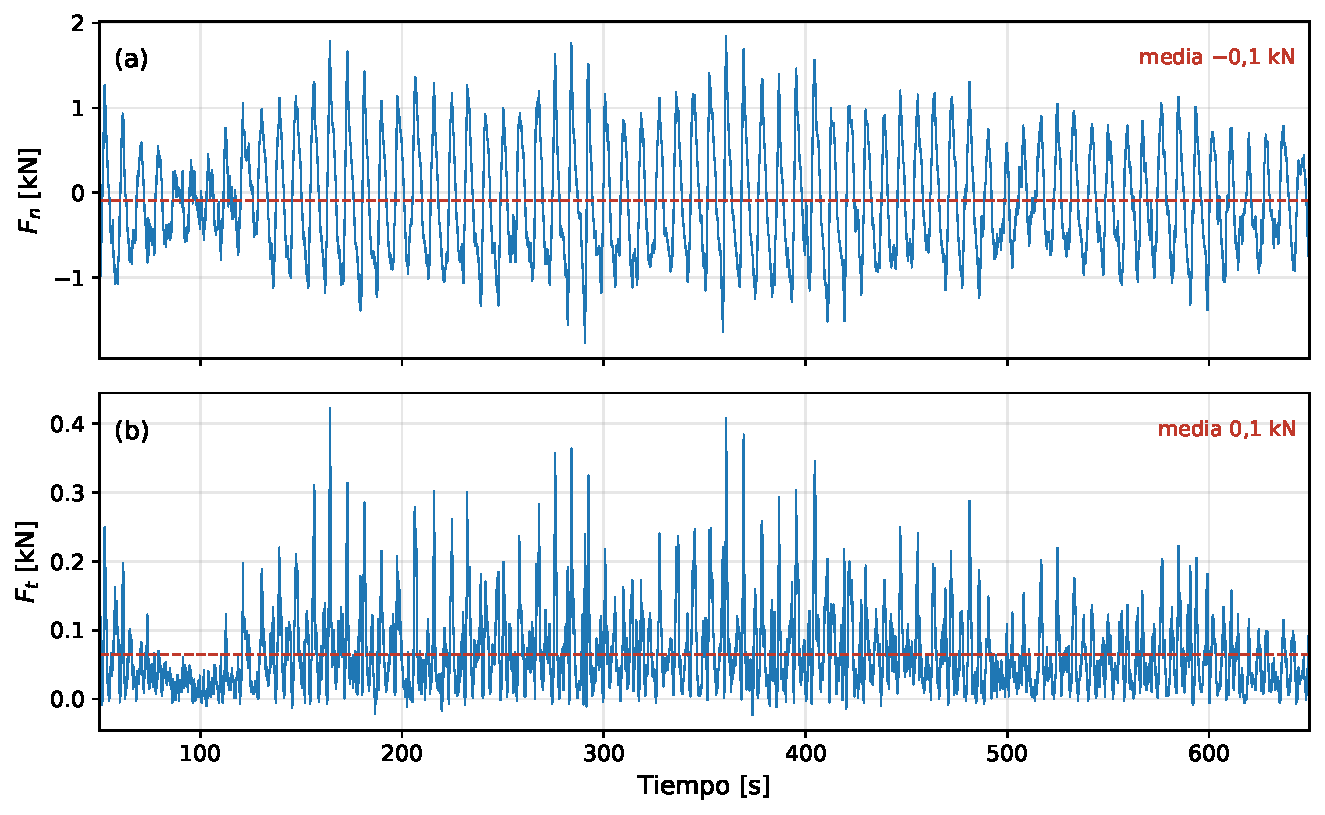
\includegraphics[width=0.85\textwidth]{Figuras/Figuras Anexo Fuerzas/fuerzas_xy_V2_S1.pdf}
    \caption{Fuerzas resultantes (a) $F_x$ y (b) $F_y$ en función del tiempo, $V = 2$~m/s, semilla $1$.}
    \label{fig:anexo_fuerzas_xy_V2_S1}
\end{figure}

\begin{figure}[H]
    \centering
    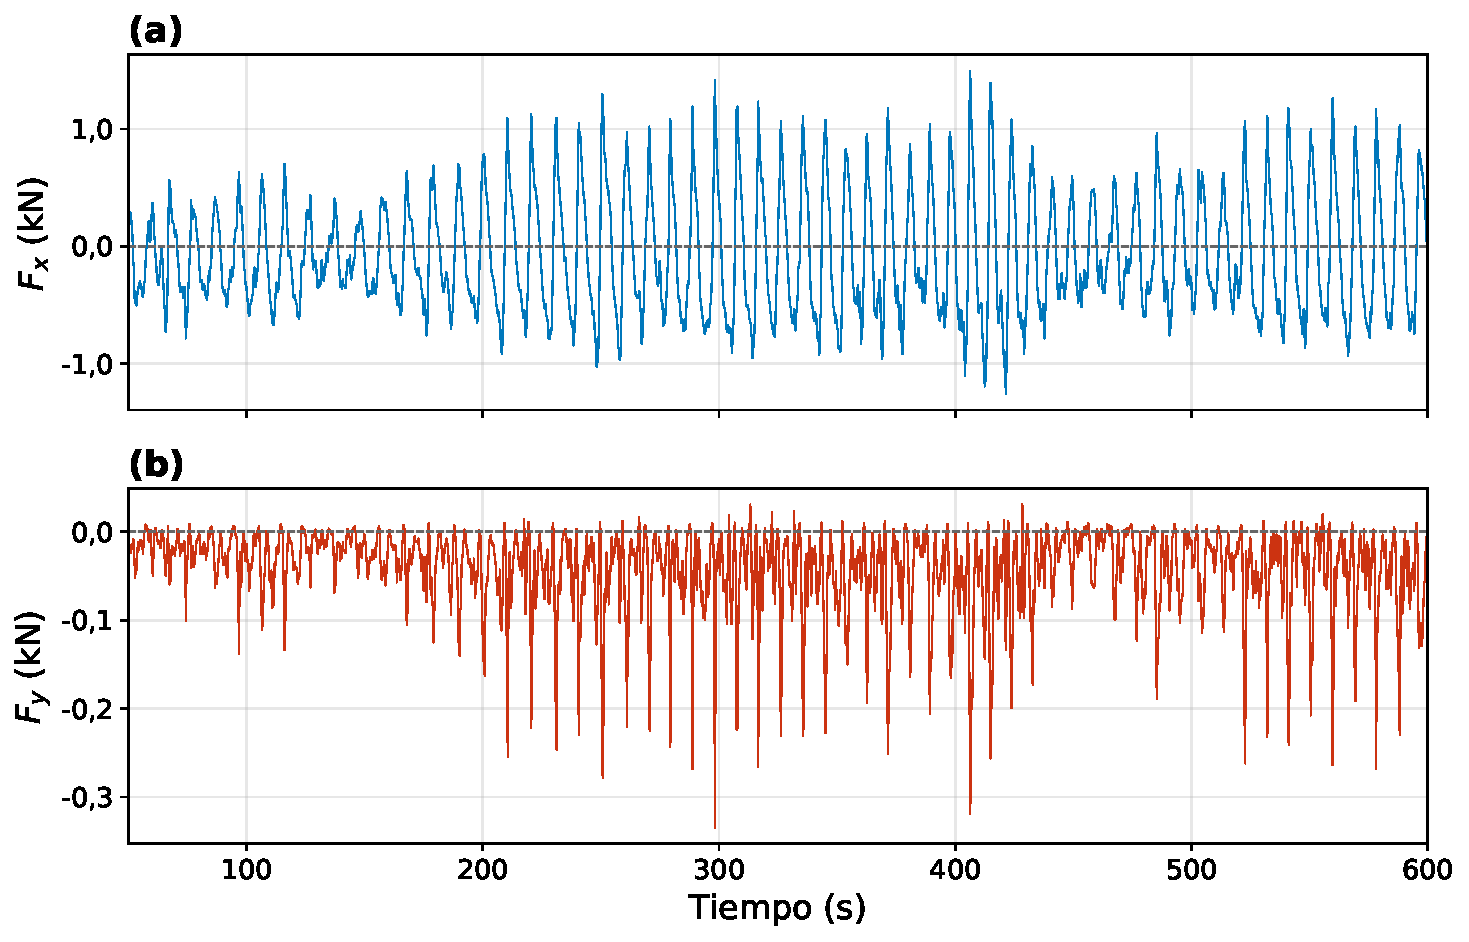
\includegraphics[width=0.85\textwidth]{Figuras/Figuras Anexo Fuerzas/fuerzas_xy_V2_S2.pdf}
    \caption{Fuerzas resultantes (a) $F_x$ y (b) $F_y$ en función del tiempo, $V = 2$~m/s, semilla $2$.}
    \label{fig:anexo_fuerzas_xy_V2_S2}
\end{figure}

\begin{figure}[H]
    \centering
    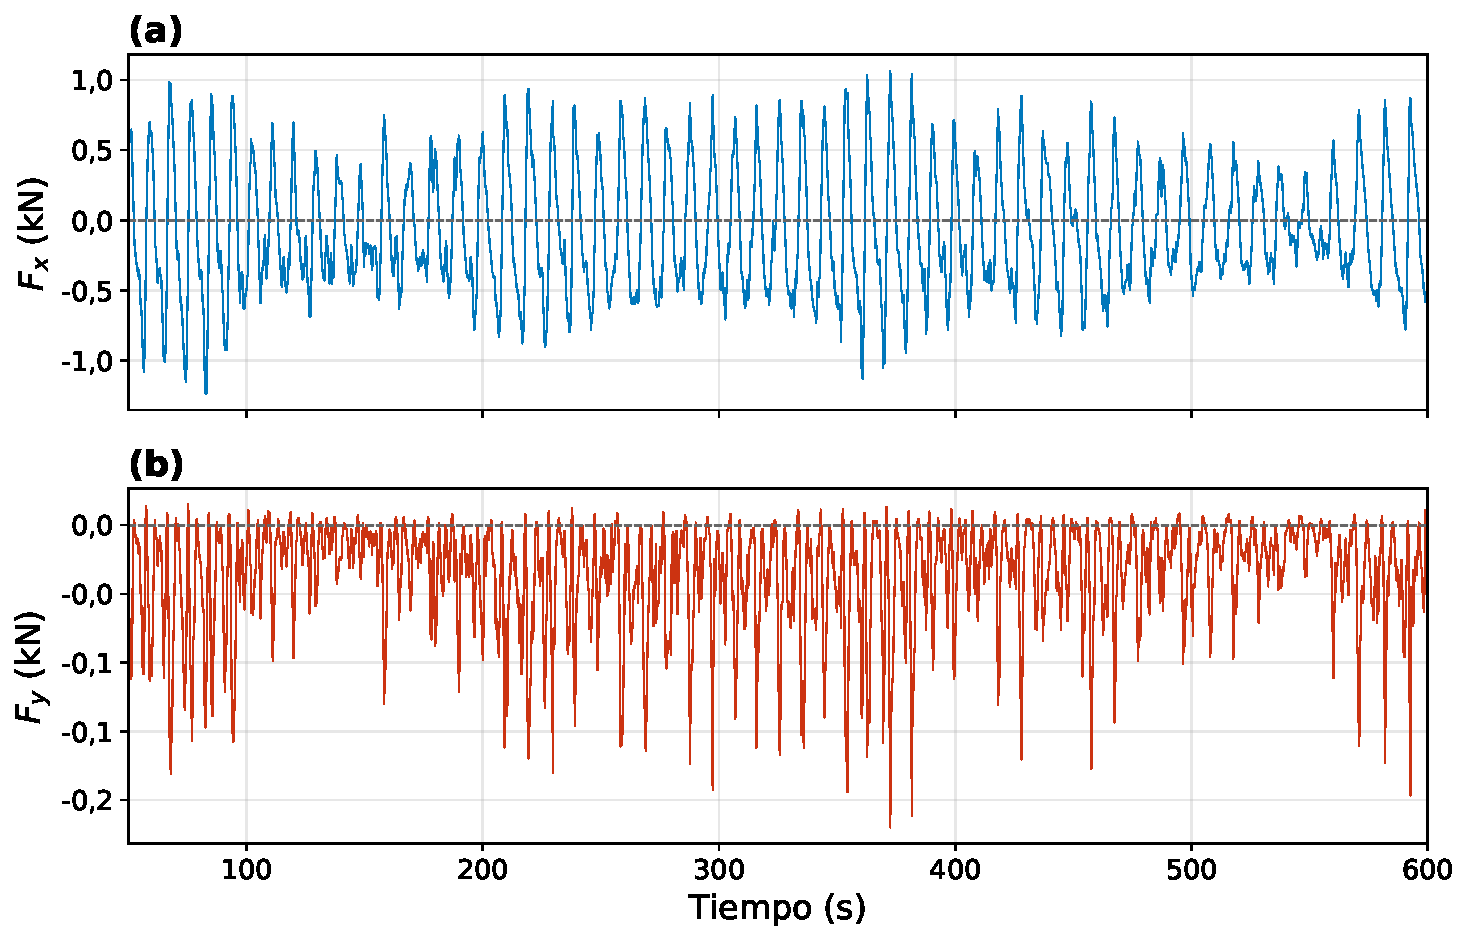
\includegraphics[width=0.85\textwidth]{Figuras/Figuras Anexo Fuerzas/fuerzas_xy_V2_S3.pdf}
    \caption{Fuerzas resultantes (a) $F_x$ y (b) $F_y$ en función del tiempo, $V = 2$~m/s, semilla $3$.}
    \label{fig:anexo_fuerzas_xy_V2_S3}
\end{figure}

\begin{figure}[H]
    \centering
    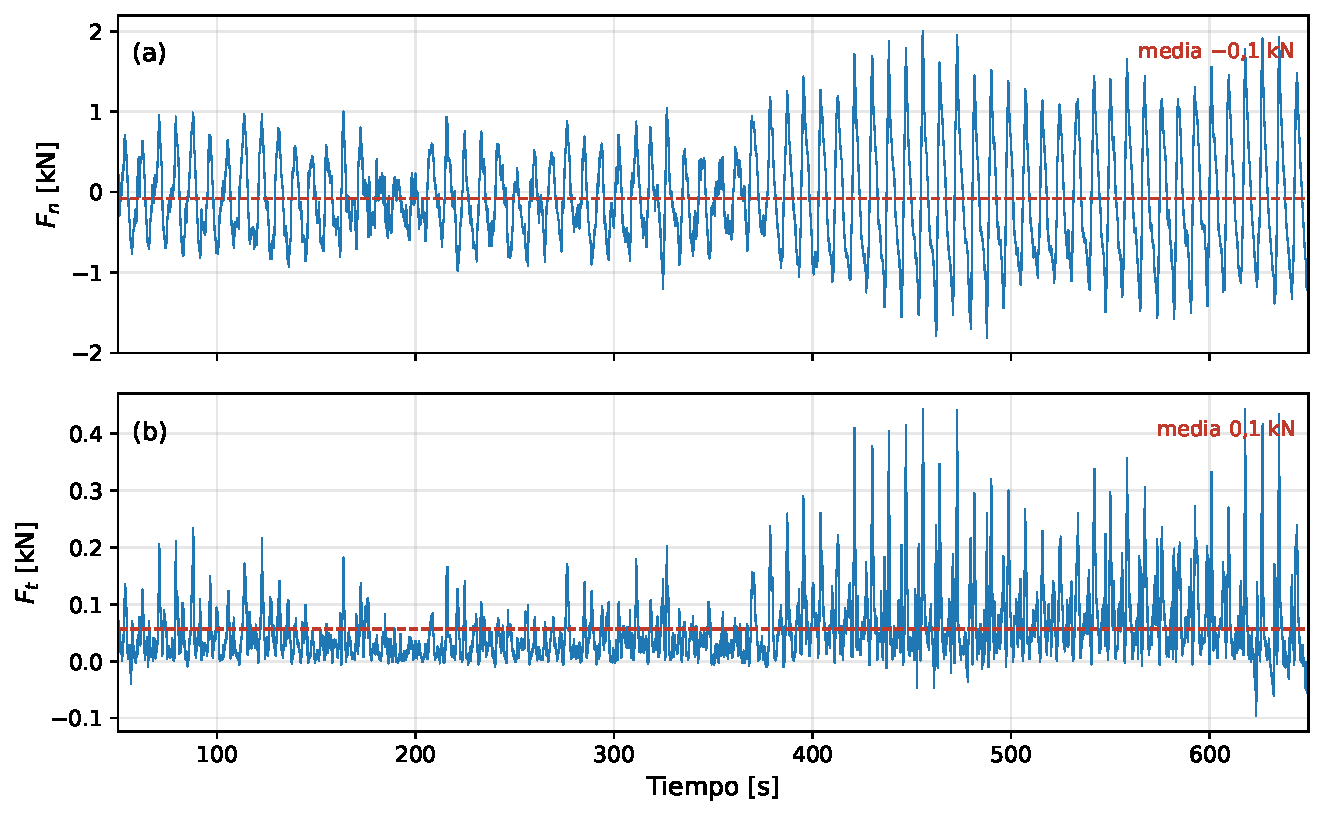
\includegraphics[width=0.85\textwidth]{Figuras/Figuras Anexo Fuerzas/fuerzas_xy_V2_S4.pdf}
    \caption{Fuerzas resultantes (a) $F_x$ y (b) $F_y$ en función del tiempo, $V = 2$~m/s, semilla $4$.}
    \label{fig:anexo_fuerzas_xy_V2_S4}
\end{figure}

\begin{figure}[H]
    \centering
    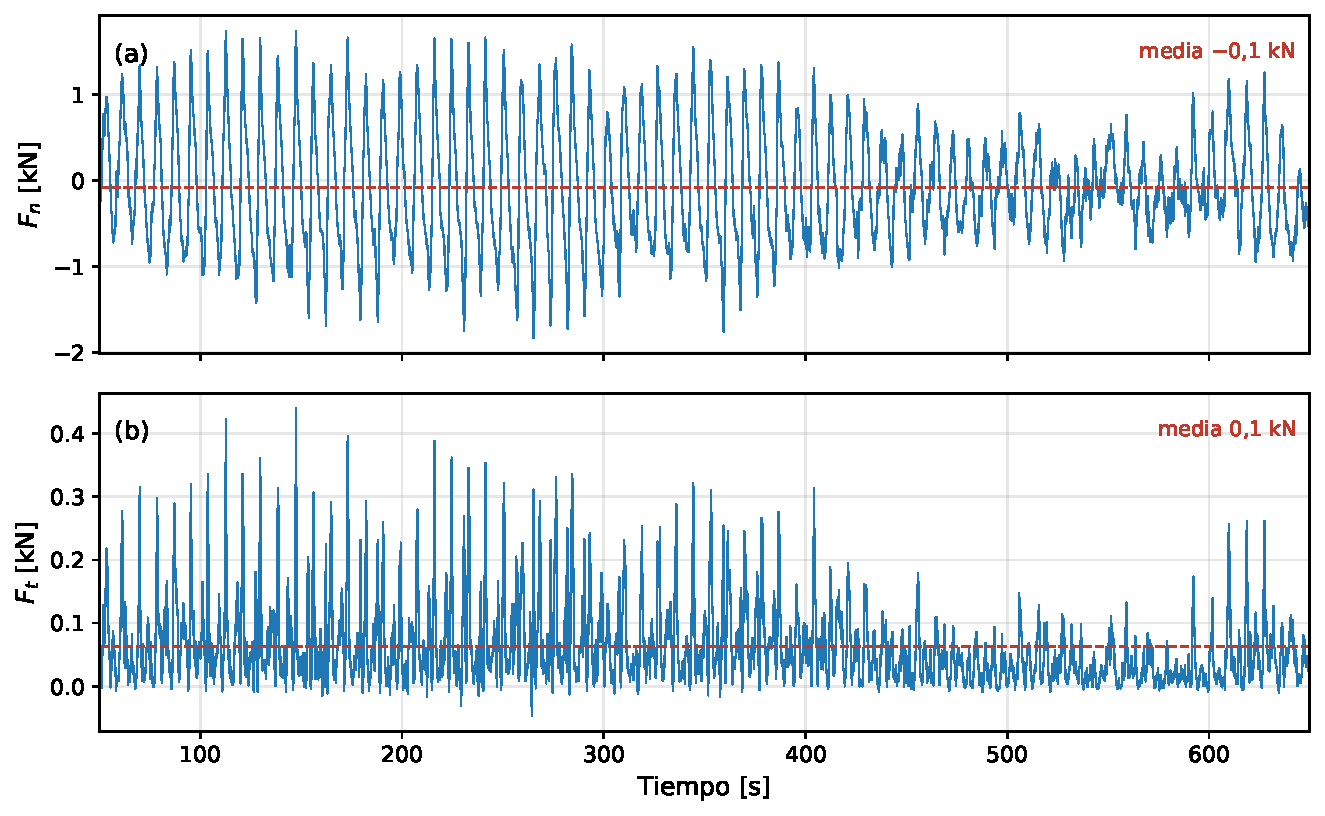
\includegraphics[width=0.85\textwidth]{Figuras/Figuras Anexo Fuerzas/fuerzas_xy_V2_S5.pdf}
    \caption{Fuerzas resultantes (a) $F_x$ y (b) $F_y$ en función del tiempo, $V = 2$~m/s, semilla $5$.}
    \label{fig:anexo_fuerzas_xy_V2_S5}
\end{figure}

\begin{figure}[H]
    \centering
    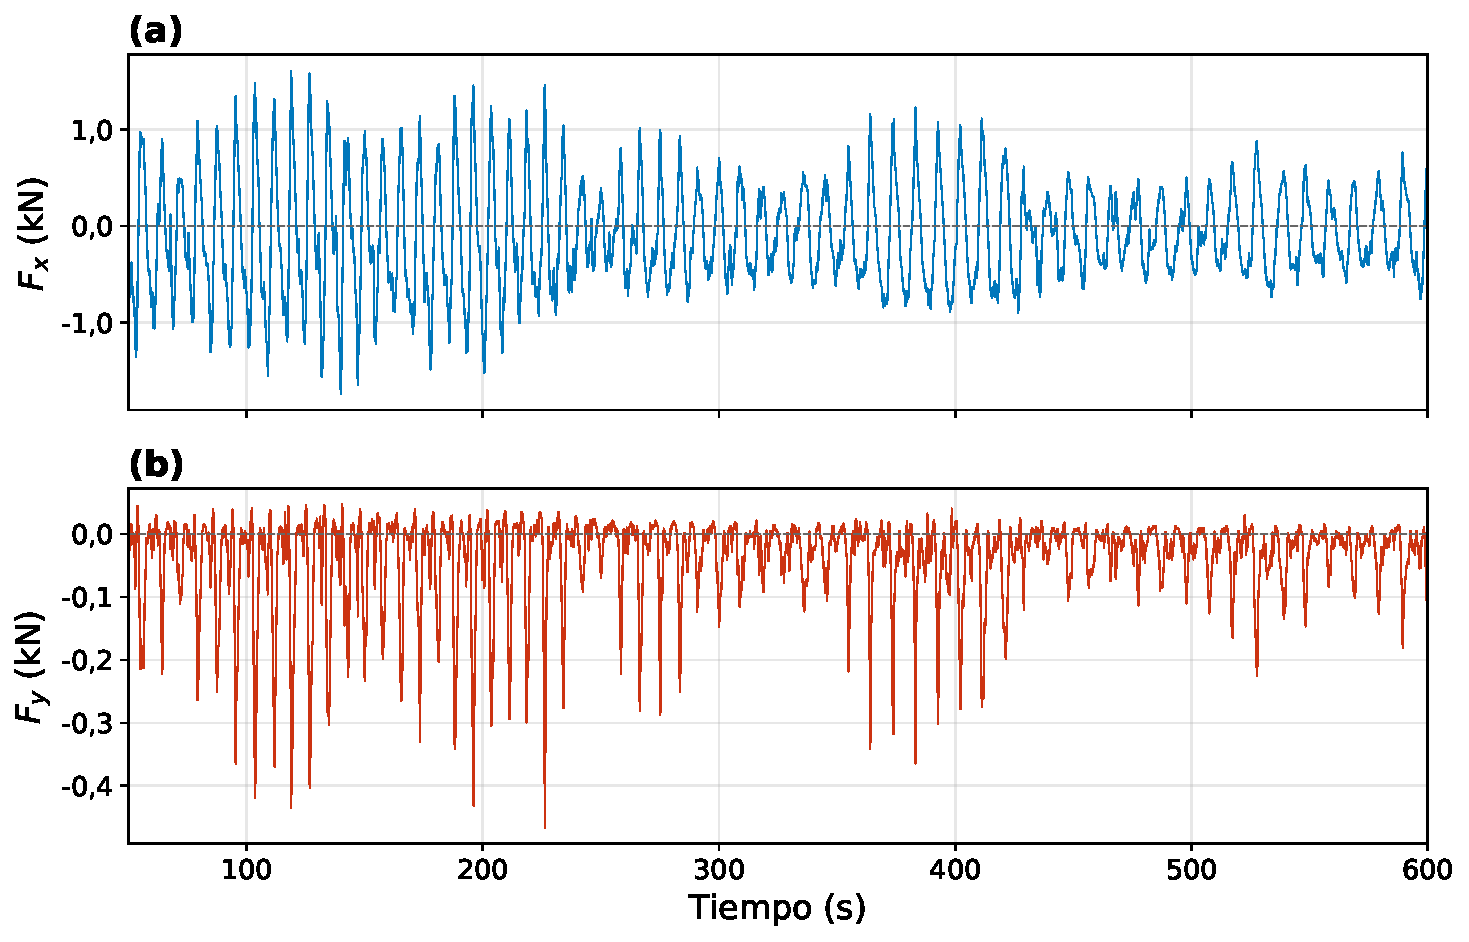
\includegraphics[width=0.85\textwidth]{Figuras/Figuras Anexo Fuerzas/fuerzas_xy_V2_S6.pdf}
    \caption{Fuerzas resultantes (a) $F_x$ y (b) $F_y$ en función del tiempo, $V = 2$~m/s, semilla $6$.}
    \label{fig:anexo_fuerzas_xy_V2_S6}
\end{figure}

\begin{figure}[H]
    \centering
    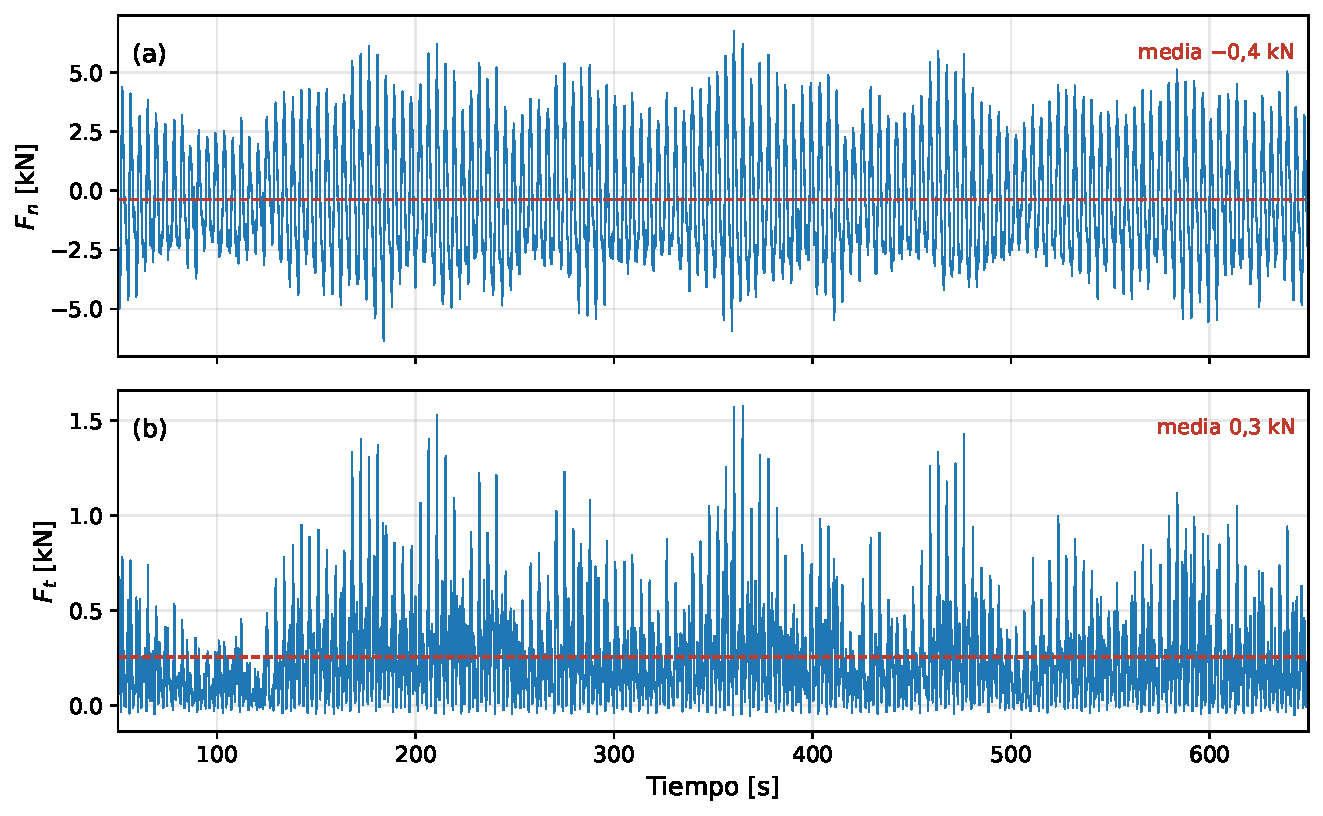
\includegraphics[width=0.85\textwidth]{Figuras/Figuras Anexo Fuerzas/fuerzas_xy_V4_S1.pdf}
    \caption{Fuerzas resultantes (a) $F_x$ y (b) $F_y$ en función del tiempo, $V = 4$~m/s, semilla $1$.}
    \label{fig:anexo_fuerzas_xy_V4_S1}
\end{figure}

\begin{figure}[H]
    \centering
    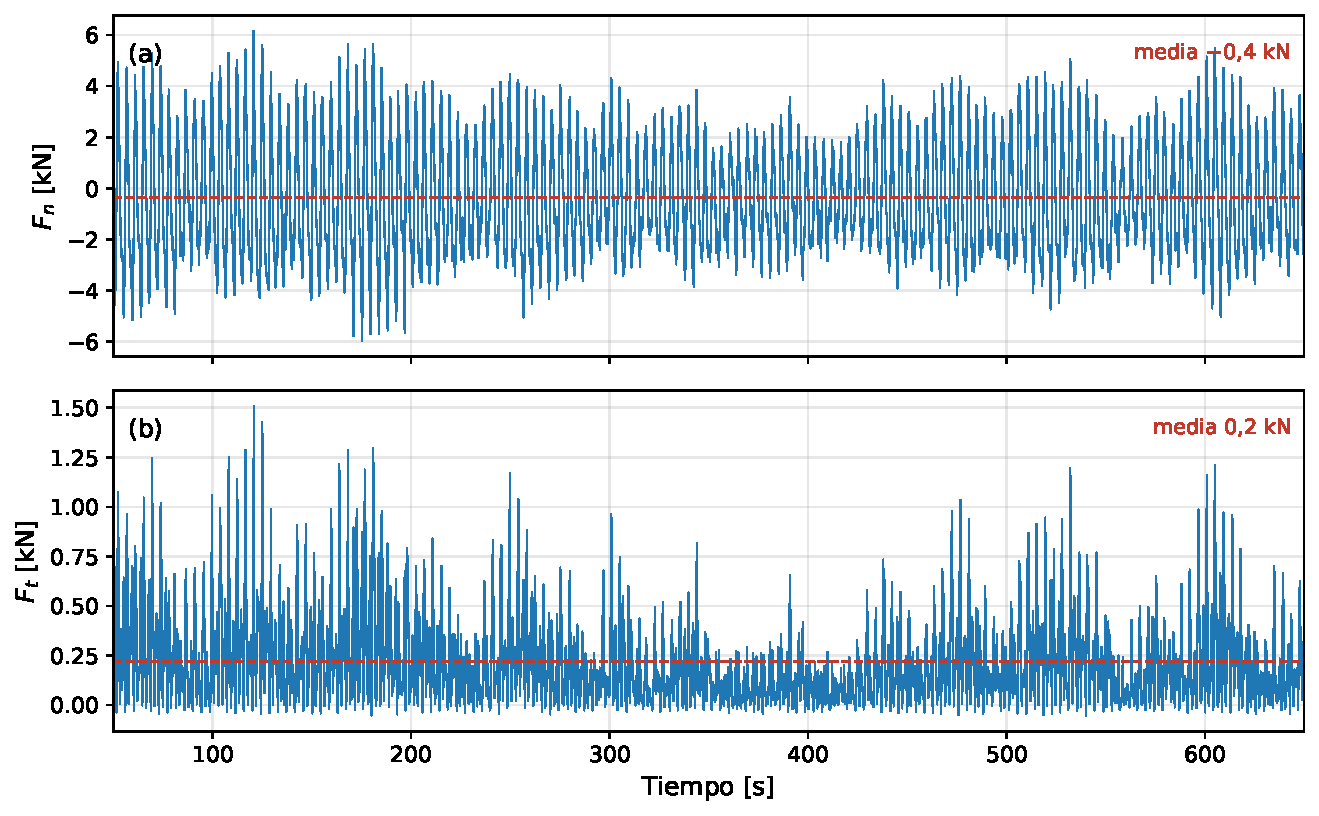
\includegraphics[width=0.85\textwidth]{Figuras/Figuras Anexo Fuerzas/fuerzas_xy_V4_S2.pdf}
    \caption{Fuerzas resultantes (a) $F_x$ y (b) $F_y$ en función del tiempo, $V = 4$~m/s, semilla $2$.}
    \label{fig:anexo_fuerzas_xy_V4_S2}
\end{figure}

\begin{figure}[H]
    \centering
    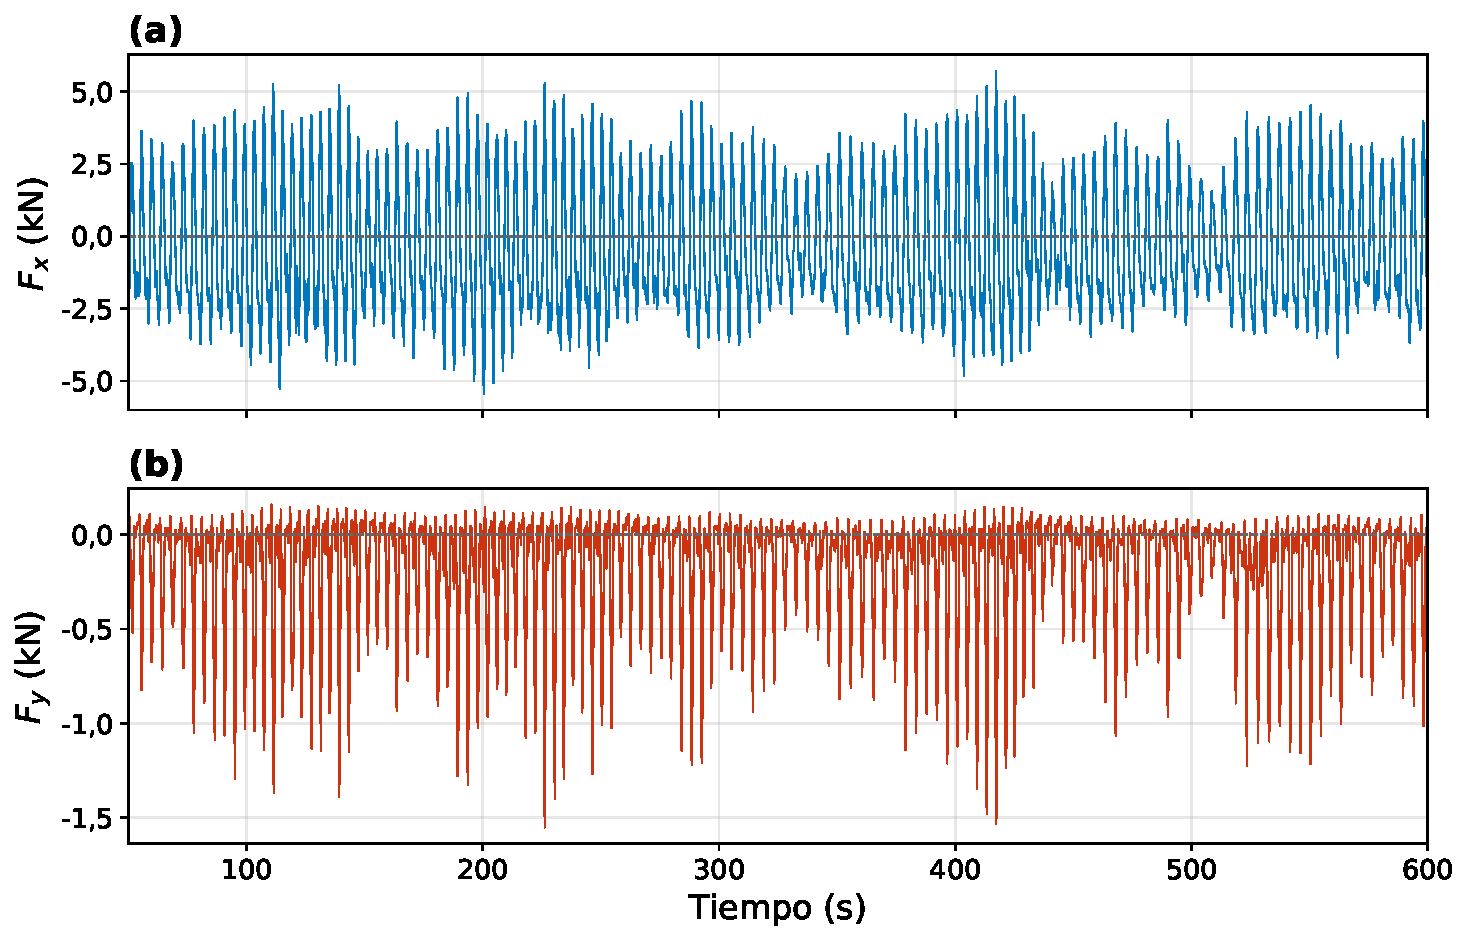
\includegraphics[width=0.85\textwidth]{Figuras/Figuras Anexo Fuerzas/fuerzas_xy_V4_S3.pdf}
    \caption{Fuerzas resultantes (a) $F_x$ y (b) $F_y$ en función del tiempo, $V = 4$~m/s, semilla $3$.}
    \label{fig:anexo_fuerzas_xy_V4_S3}
\end{figure}

\begin{figure}[H]
    \centering
    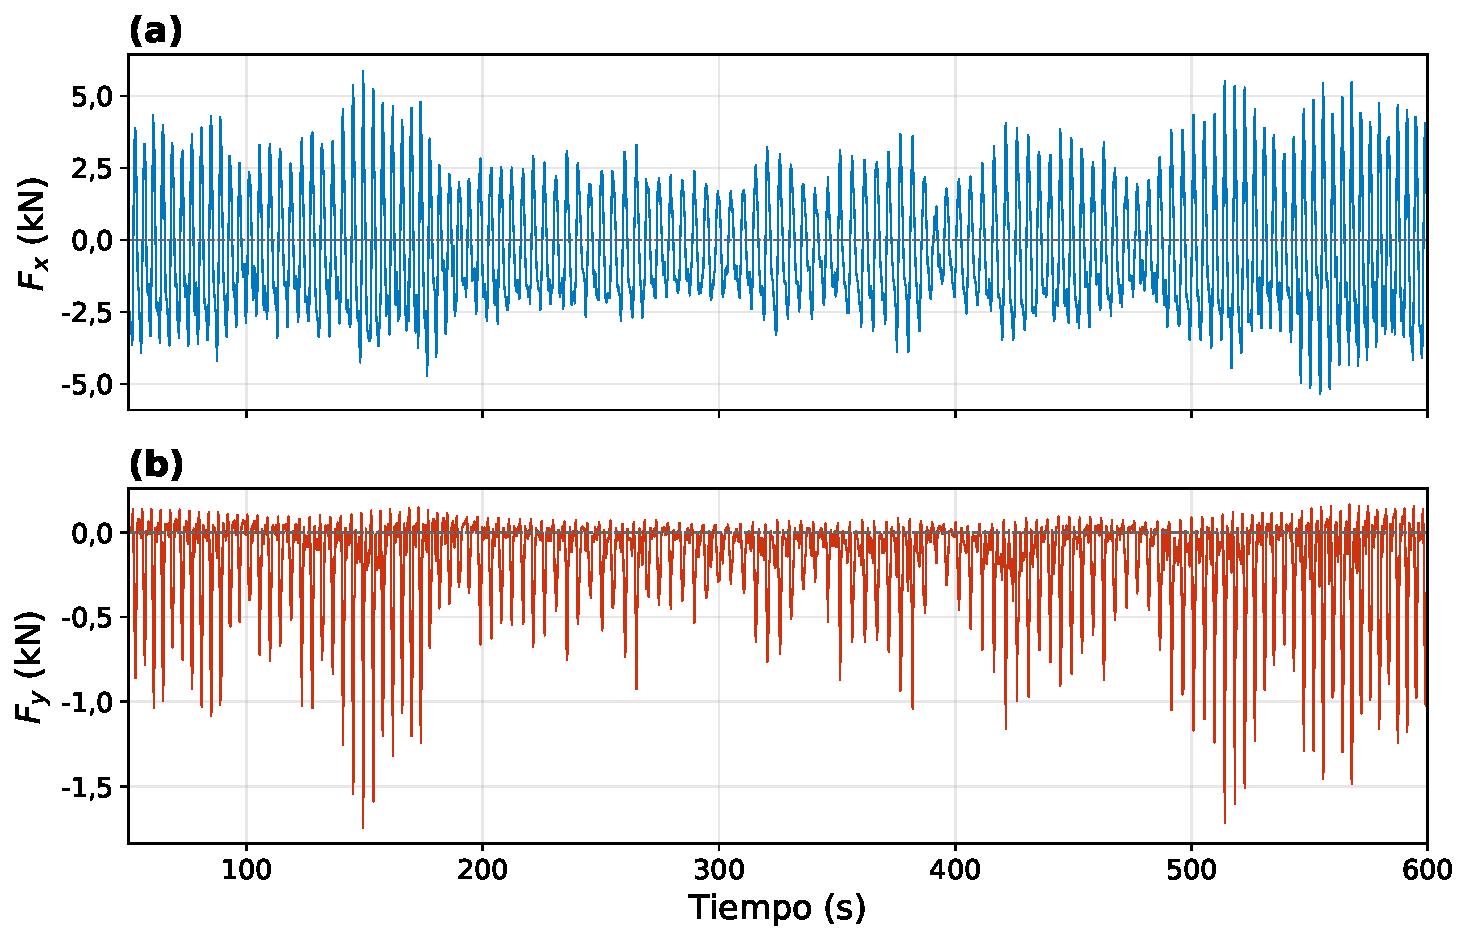
\includegraphics[width=0.85\textwidth]{Figuras/Figuras Anexo Fuerzas/fuerzas_xy_V4_S4.pdf}
    \caption{Fuerzas resultantes (a) $F_x$ y (b) $F_y$ en función del tiempo, $V = 4$~m/s, semilla $4$.}
    \label{fig:anexo_fuerzas_xy_V4_S4}
\end{figure}

\begin{figure}[H]
    \centering
    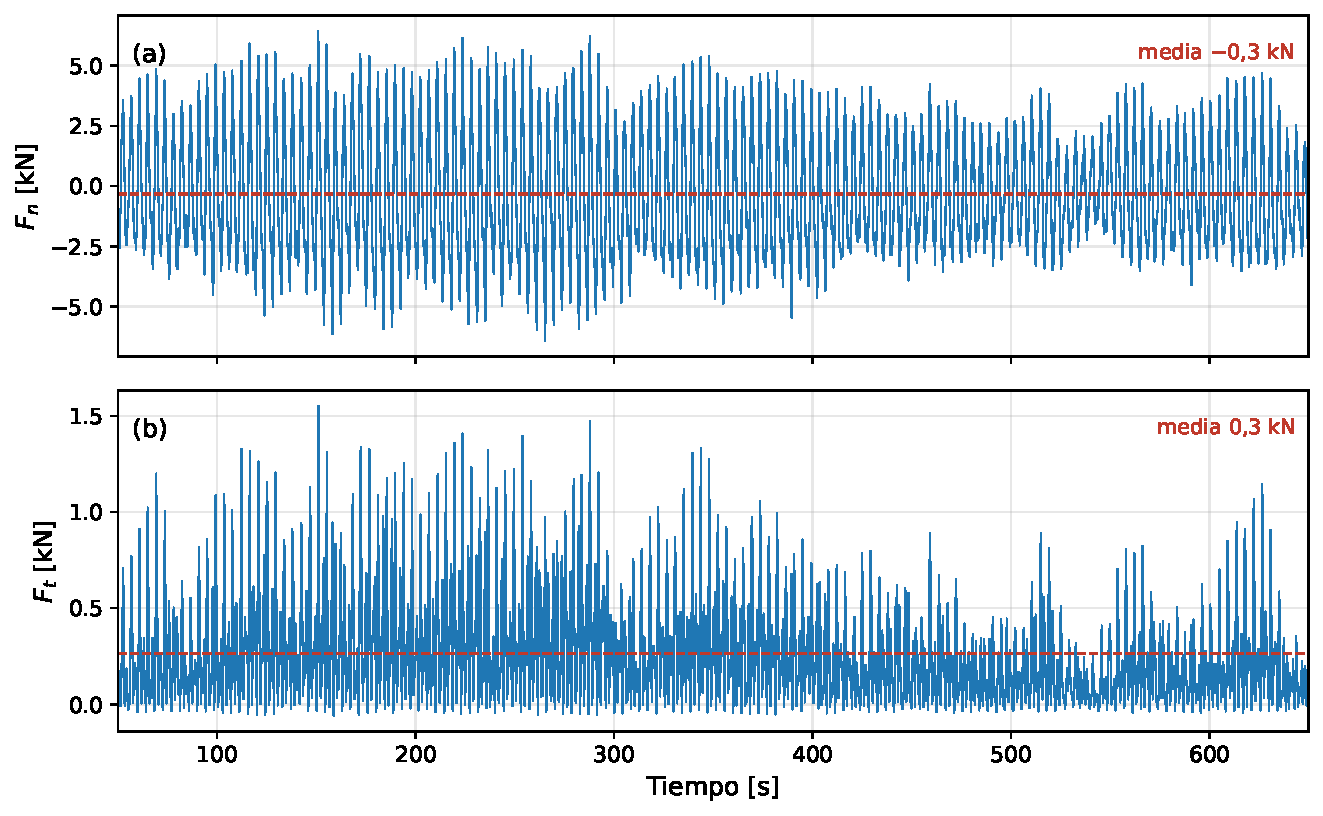
\includegraphics[width=0.85\textwidth]{Figuras/Figuras Anexo Fuerzas/fuerzas_xy_V4_S5.pdf}
    \caption{Fuerzas resultantes (a) $F_x$ y (b) $F_y$ en función del tiempo, $V = 4$~m/s, semilla $5$.}
    \label{fig:anexo_fuerzas_xy_V4_S5}
\end{figure}

\begin{figure}[H]
    \centering
    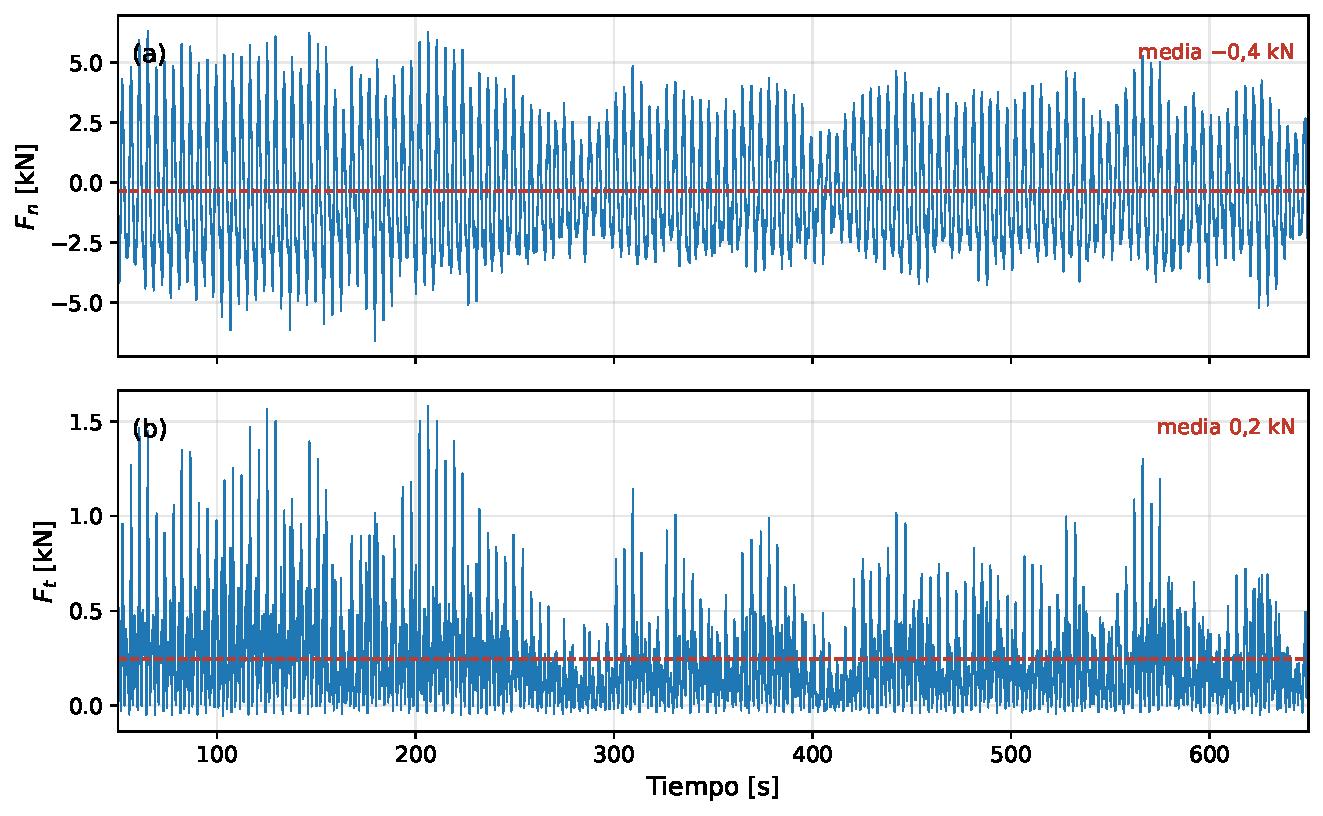
\includegraphics[width=0.85\textwidth]{Figuras/Figuras Anexo Fuerzas/fuerzas_xy_V4_S6.pdf}
    \caption{Fuerzas resultantes (a) $F_x$ y (b) $F_y$ en función del tiempo, $V = 4$~m/s, semilla $6$.}
    \label{fig:anexo_fuerzas_xy_V4_S6}
\end{figure}

\begin{figure}[H]
    \centering
    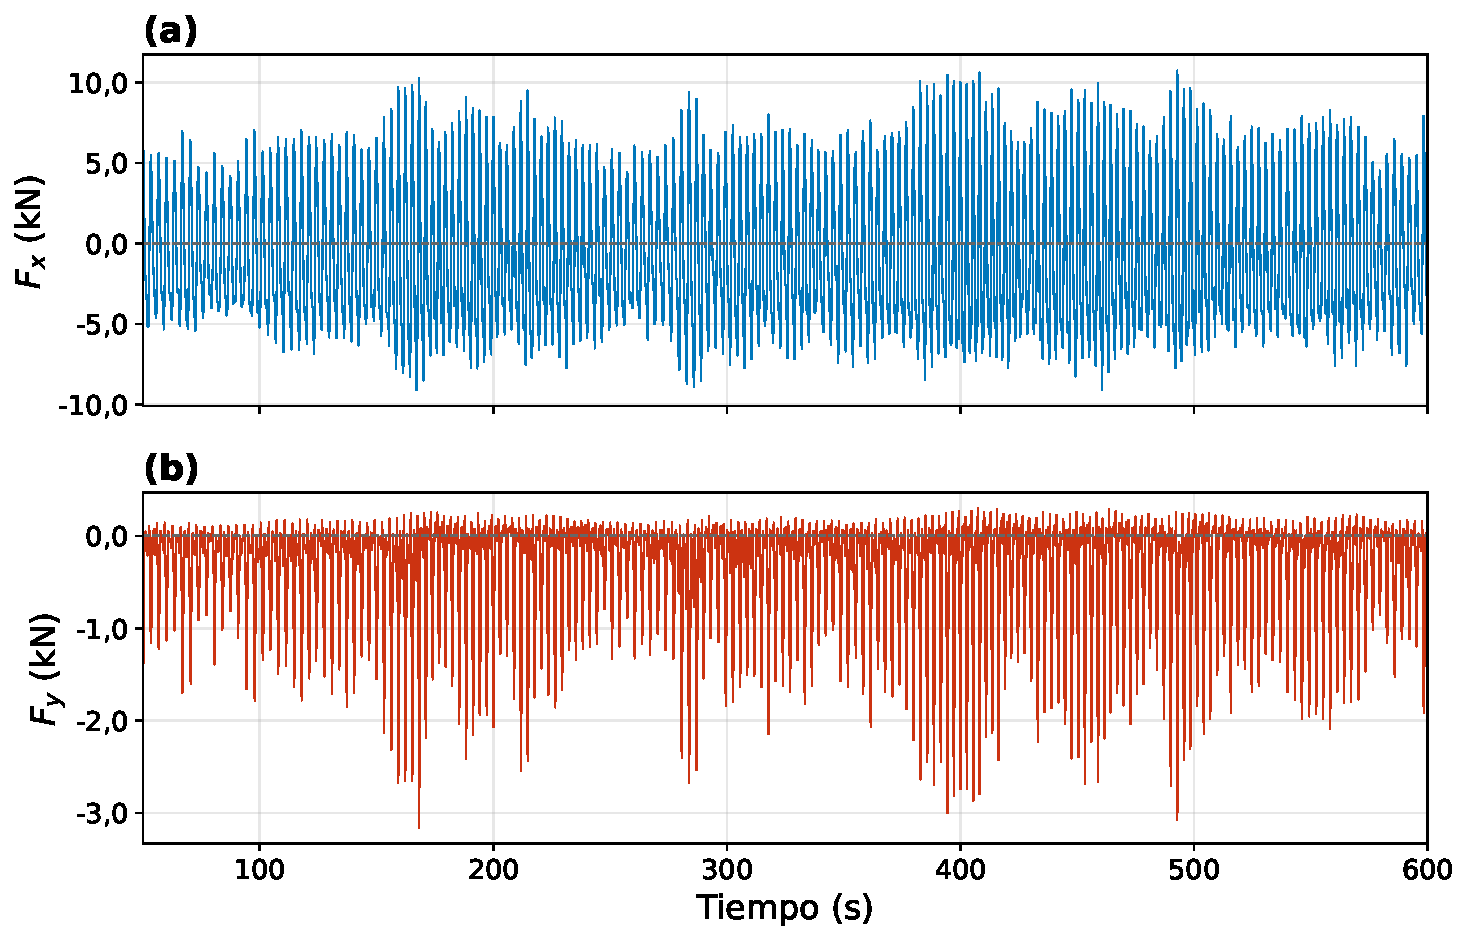
\includegraphics[width=0.85\textwidth]{Figuras/Figuras Anexo Fuerzas/fuerzas_xy_V6_S1.pdf}
    \caption{Fuerzas resultantes (a) $F_x$ y (b) $F_y$ en función del tiempo, $V = 6$~m/s, semilla $1$.}
    \label{fig:anexo_fuerzas_xy_V6_S1}
\end{figure}

\begin{figure}[H]
    \centering
    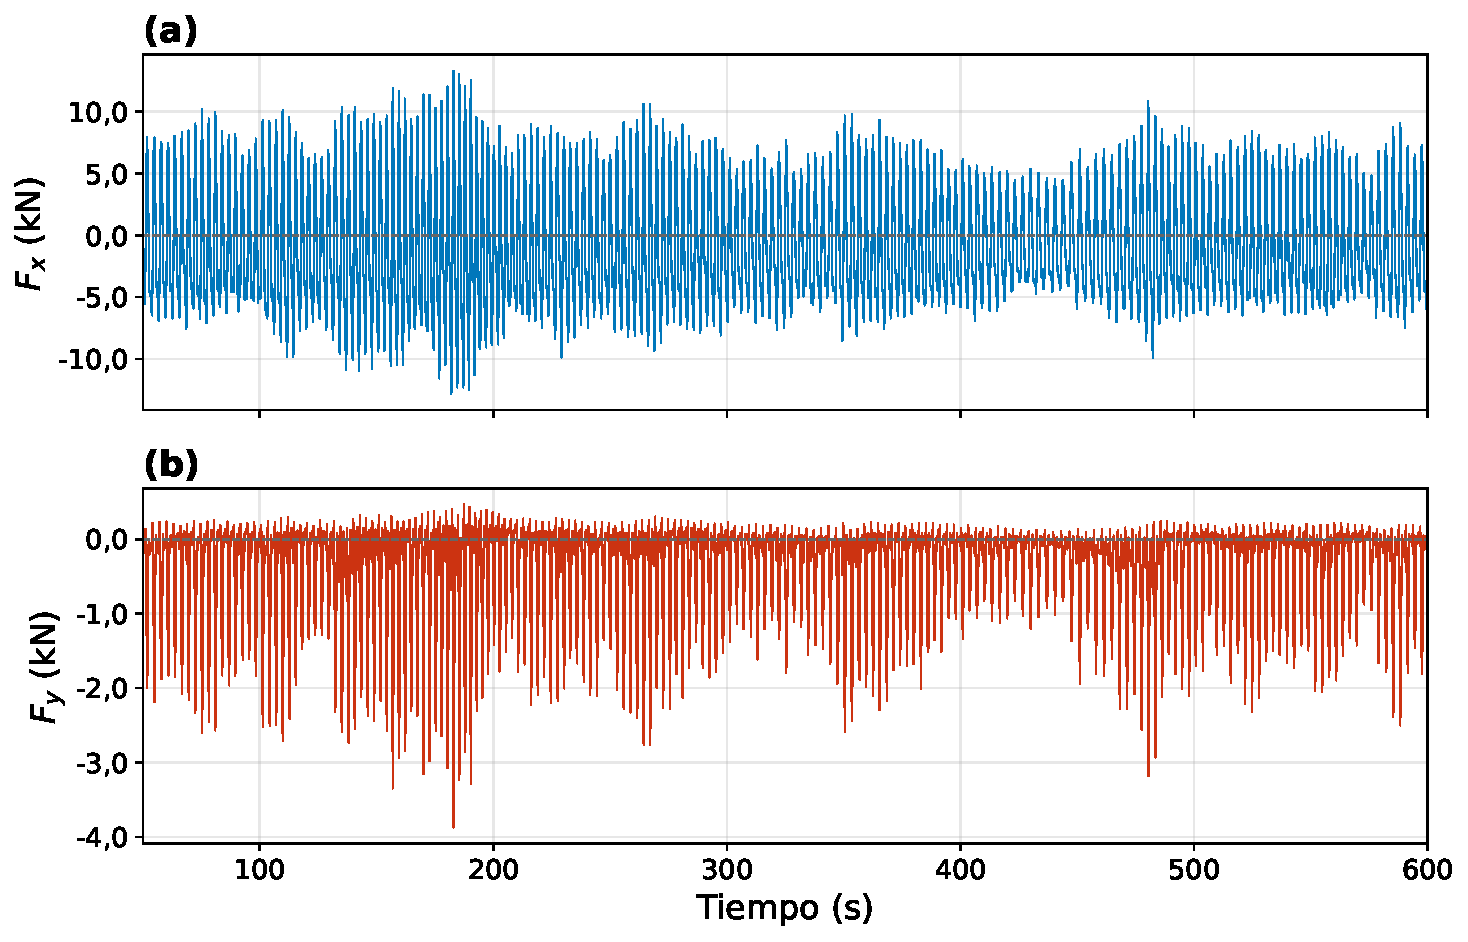
\includegraphics[width=0.85\textwidth]{Figuras/Figuras Anexo Fuerzas/fuerzas_xy_V6_S2.pdf}
    \caption{Fuerzas resultantes (a) $F_x$ y (b) $F_y$ en función del tiempo, $V = 6$~m/s, semilla $2$.}
    \label{fig:anexo_fuerzas_xy_V6_S2}
\end{figure}

\begin{figure}[H]
    \centering
    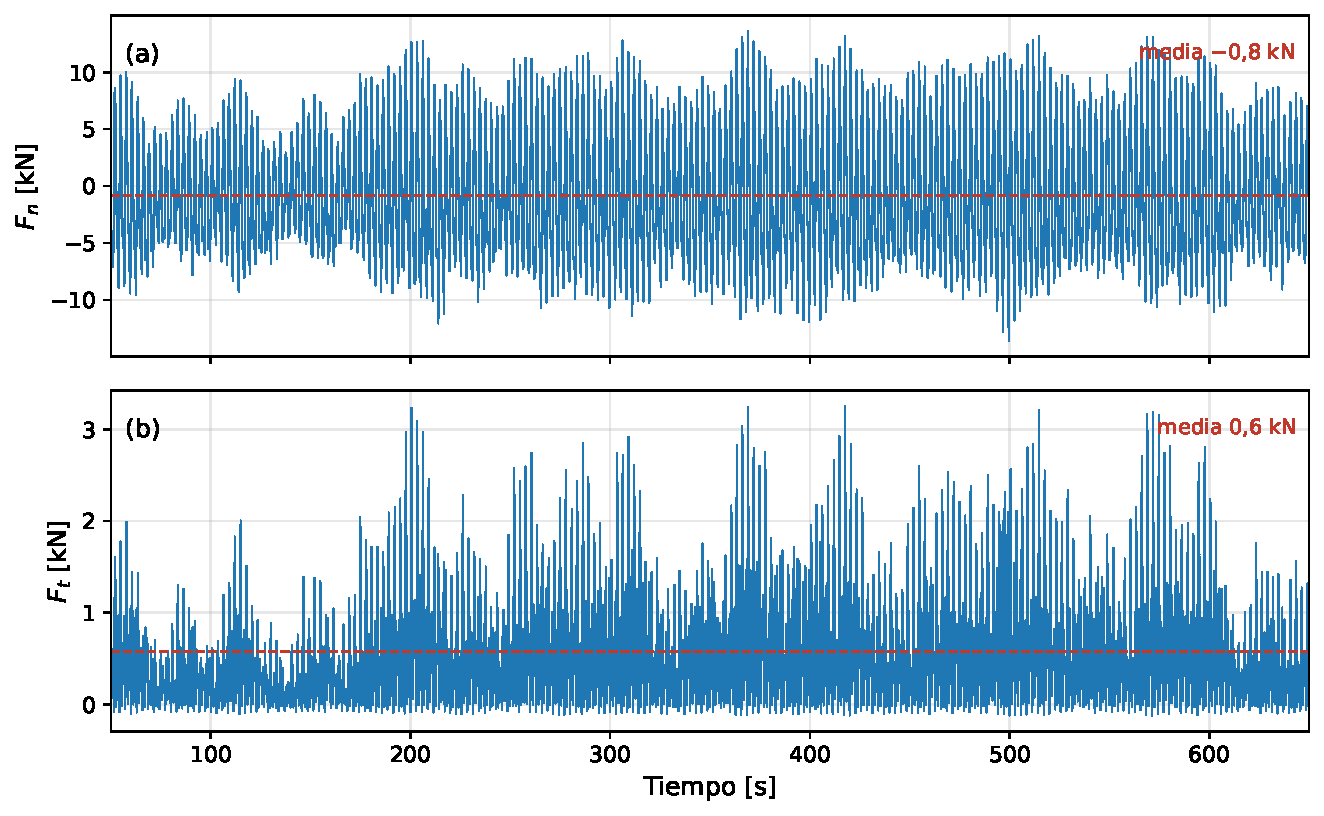
\includegraphics[width=0.85\textwidth]{Figuras/Figuras Anexo Fuerzas/fuerzas_xy_V6_S3.pdf}
    \caption{Fuerzas resultantes (a) $F_x$ y (b) $F_y$ en función del tiempo, $V = 6$~m/s, semilla $3$.}
    \label{fig:anexo_fuerzas_xy_V6_S3}
\end{figure}

\begin{figure}[H]
    \centering
    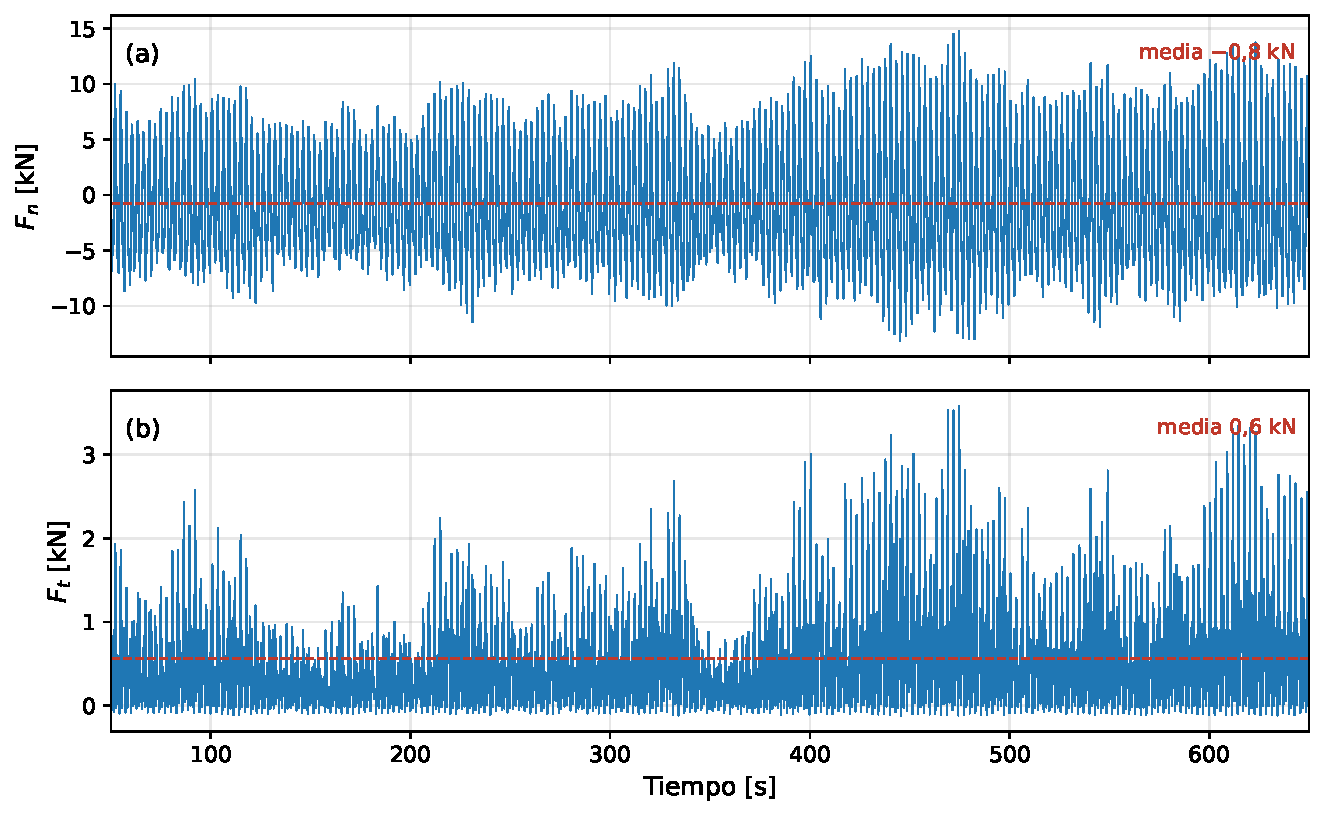
\includegraphics[width=0.85\textwidth]{Figuras/Figuras Anexo Fuerzas/fuerzas_xy_V6_S4.pdf}
    \caption{Fuerzas resultantes (a) $F_x$ y (b) $F_y$ en función del tiempo, $V = 6$~m/s, semilla $4$.}
    \label{fig:anexo_fuerzas_xy_V6_S4}
\end{figure}

\begin{figure}[H]
    \centering
    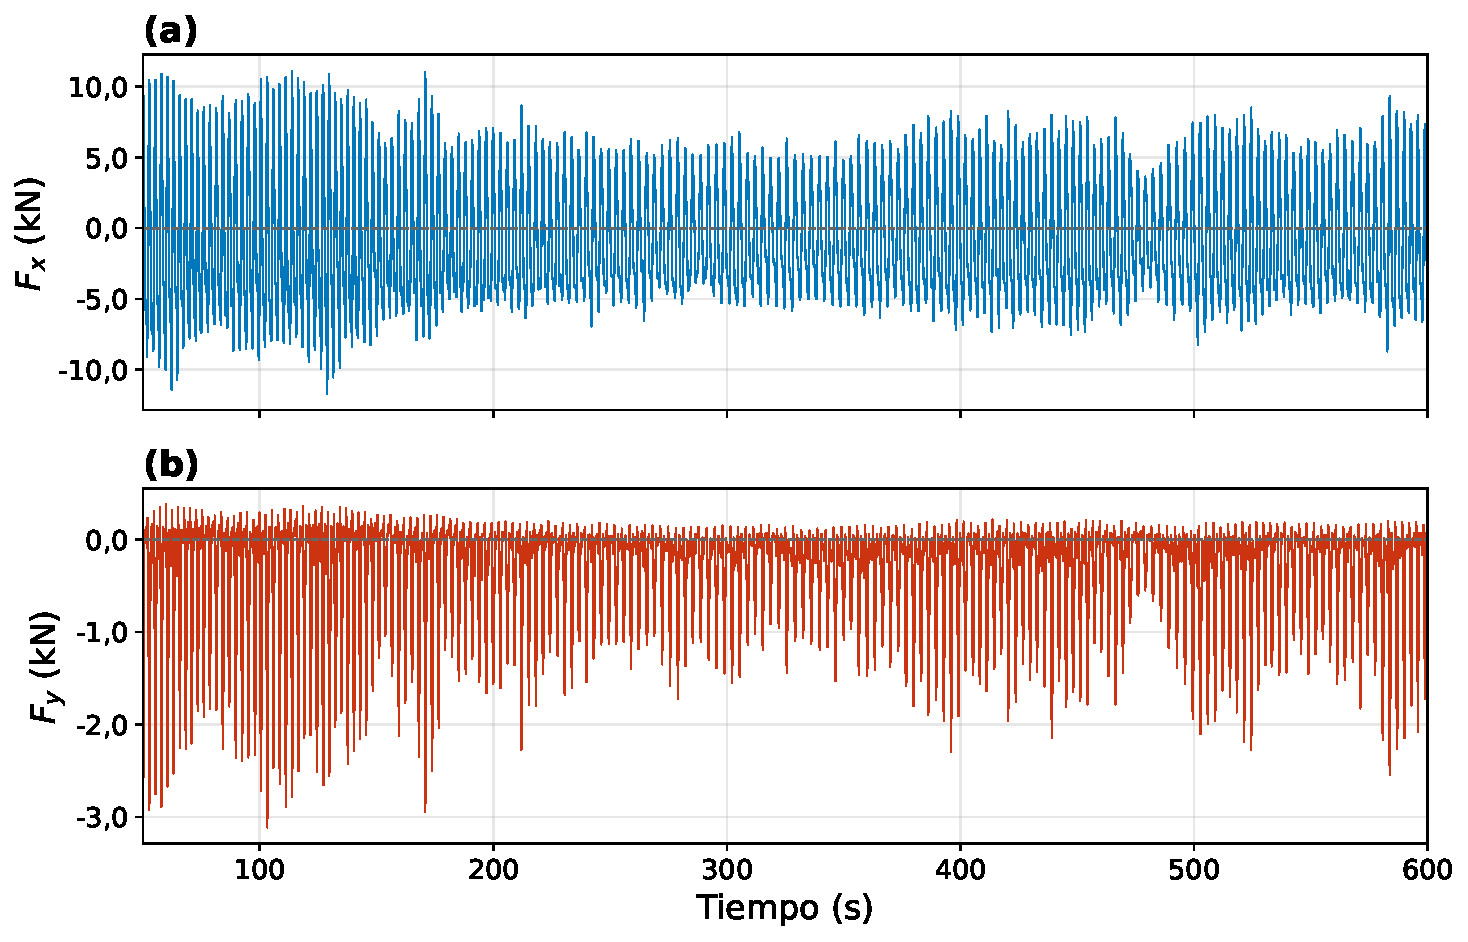
\includegraphics[width=0.85\textwidth]{Figuras/Figuras Anexo Fuerzas/fuerzas_xy_V6_S5.pdf}
    \caption{Fuerzas resultantes (a) $F_x$ y (b) $F_y$ en función del tiempo, $V = 6$~m/s, semilla $5$.}
    \label{fig:anexo_fuerzas_xy_V6_S5}
\end{figure}

\begin{figure}[H]
    \centering
    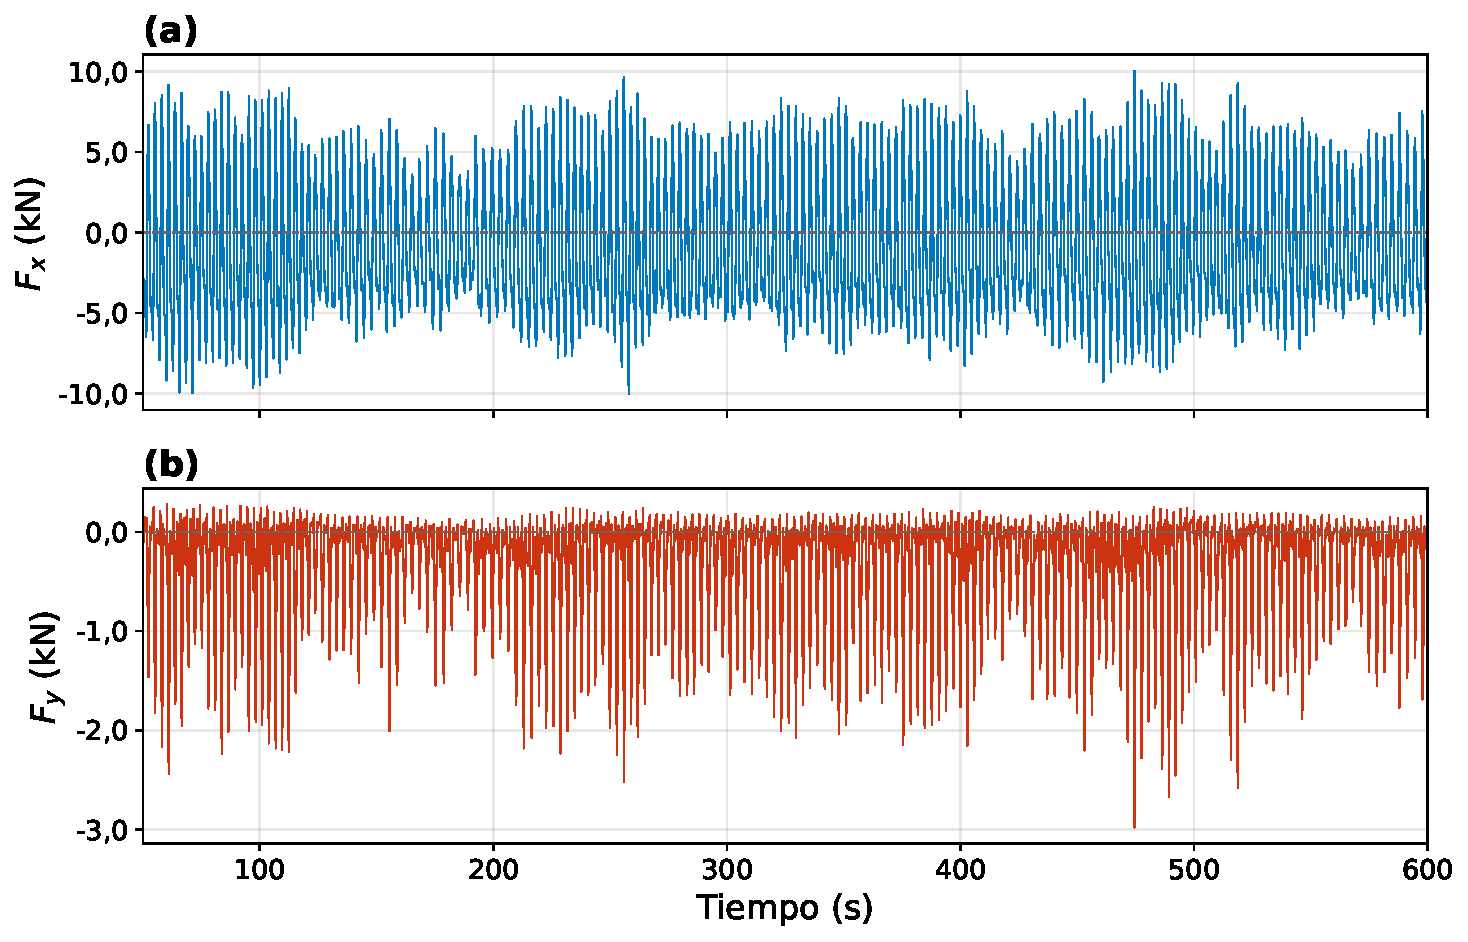
\includegraphics[width=0.85\textwidth]{Figuras/Figuras Anexo Fuerzas/fuerzas_xy_V6_S6.pdf}
    \caption{Fuerzas resultantes (a) $F_x$ y (b) $F_y$ en función del tiempo, $V = 6$~m/s, semilla $6$.}
    \label{fig:anexo_fuerzas_xy_V6_S6}
\end{figure}

\begin{figure}[H]
    \centering
    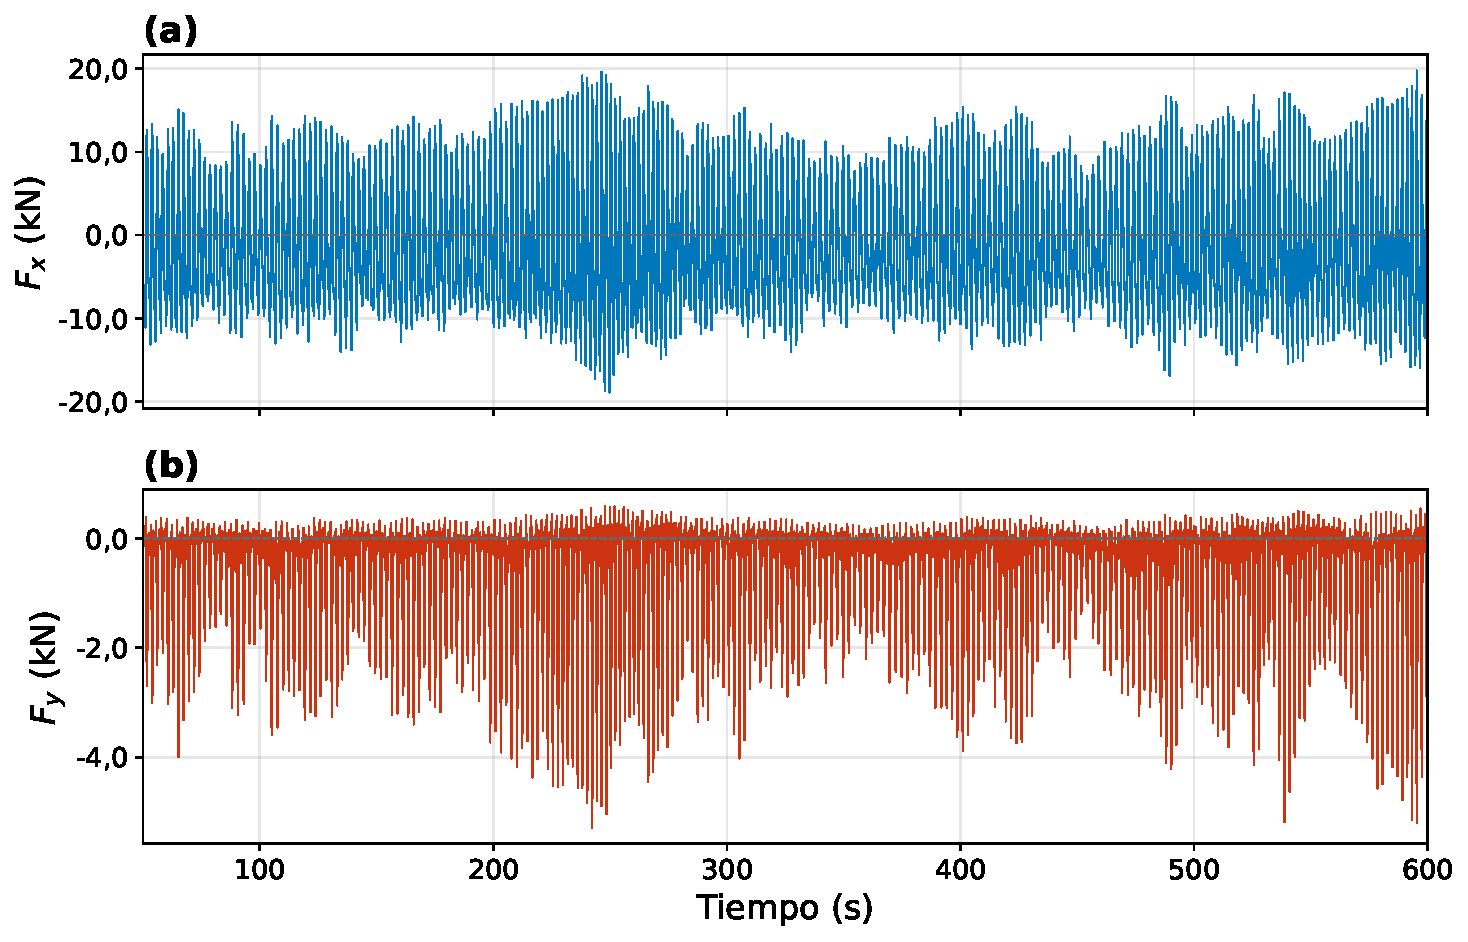
\includegraphics[width=0.85\textwidth]{Figuras/Figuras Anexo Fuerzas/fuerzas_xy_V8_S1.pdf}
    \caption{Fuerzas resultantes (a) $F_x$ y (b) $F_y$ en función del tiempo, $V = 8$~m/s, semilla $1$.}
    \label{fig:anexo_fuerzas_xy_V8_S1}
\end{figure}

\begin{figure}[H]
    \centering
    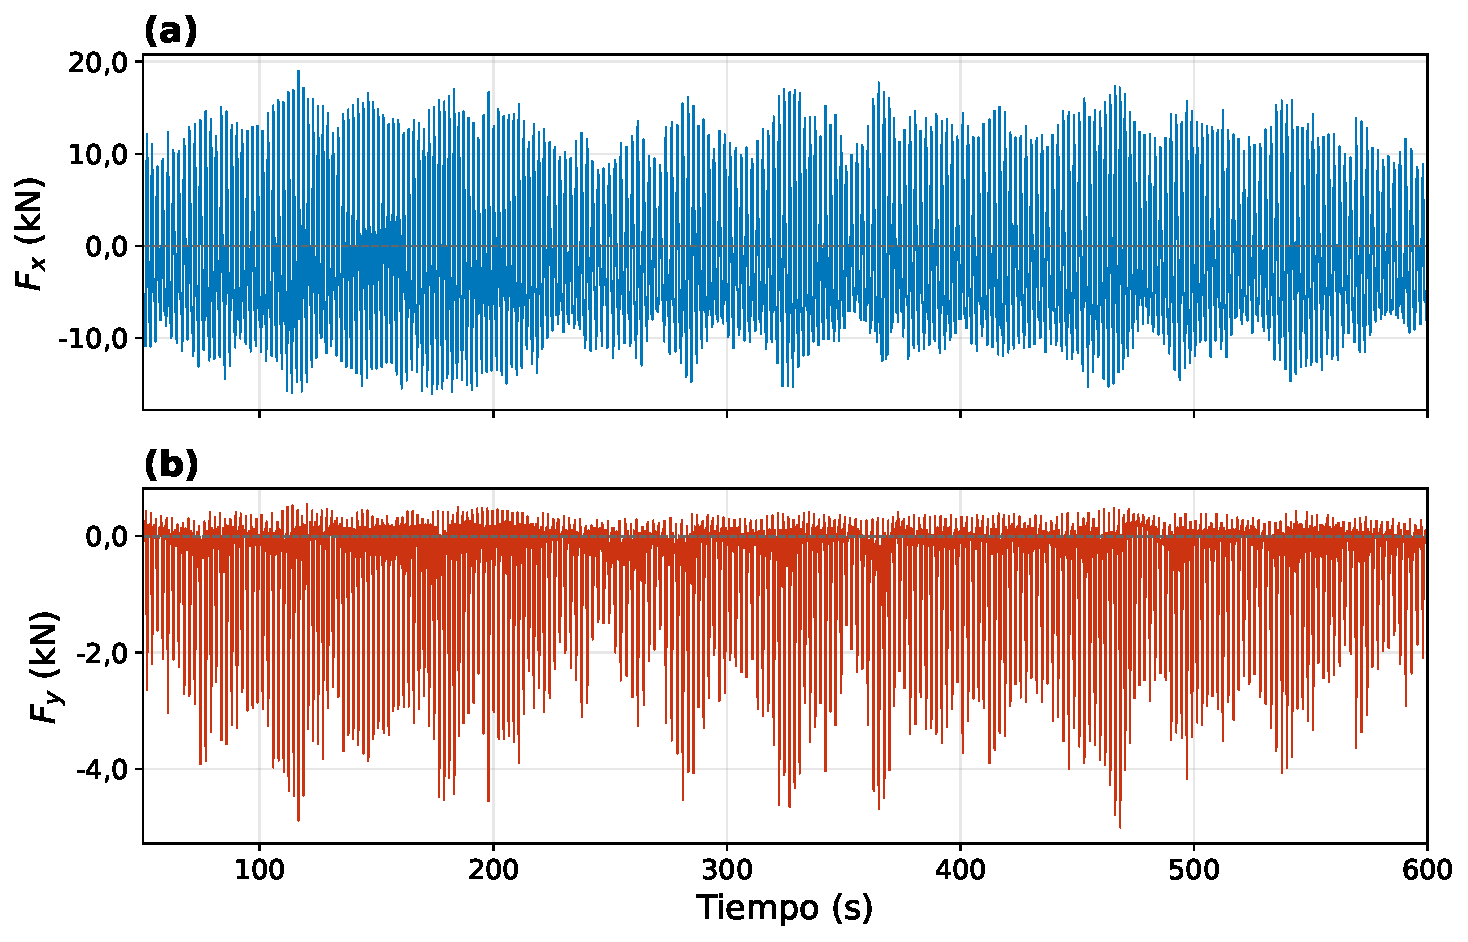
\includegraphics[width=0.85\textwidth]{Figuras/Figuras Anexo Fuerzas/fuerzas_xy_V8_S2.pdf}
    \caption{Fuerzas resultantes (a) $F_x$ y (b) $F_y$ en función del tiempo, $V = 8$~m/s, semilla $2$.}
    \label{fig:anexo_fuerzas_xy_V8_S2}
\end{figure}

\begin{figure}[H]
    \centering
    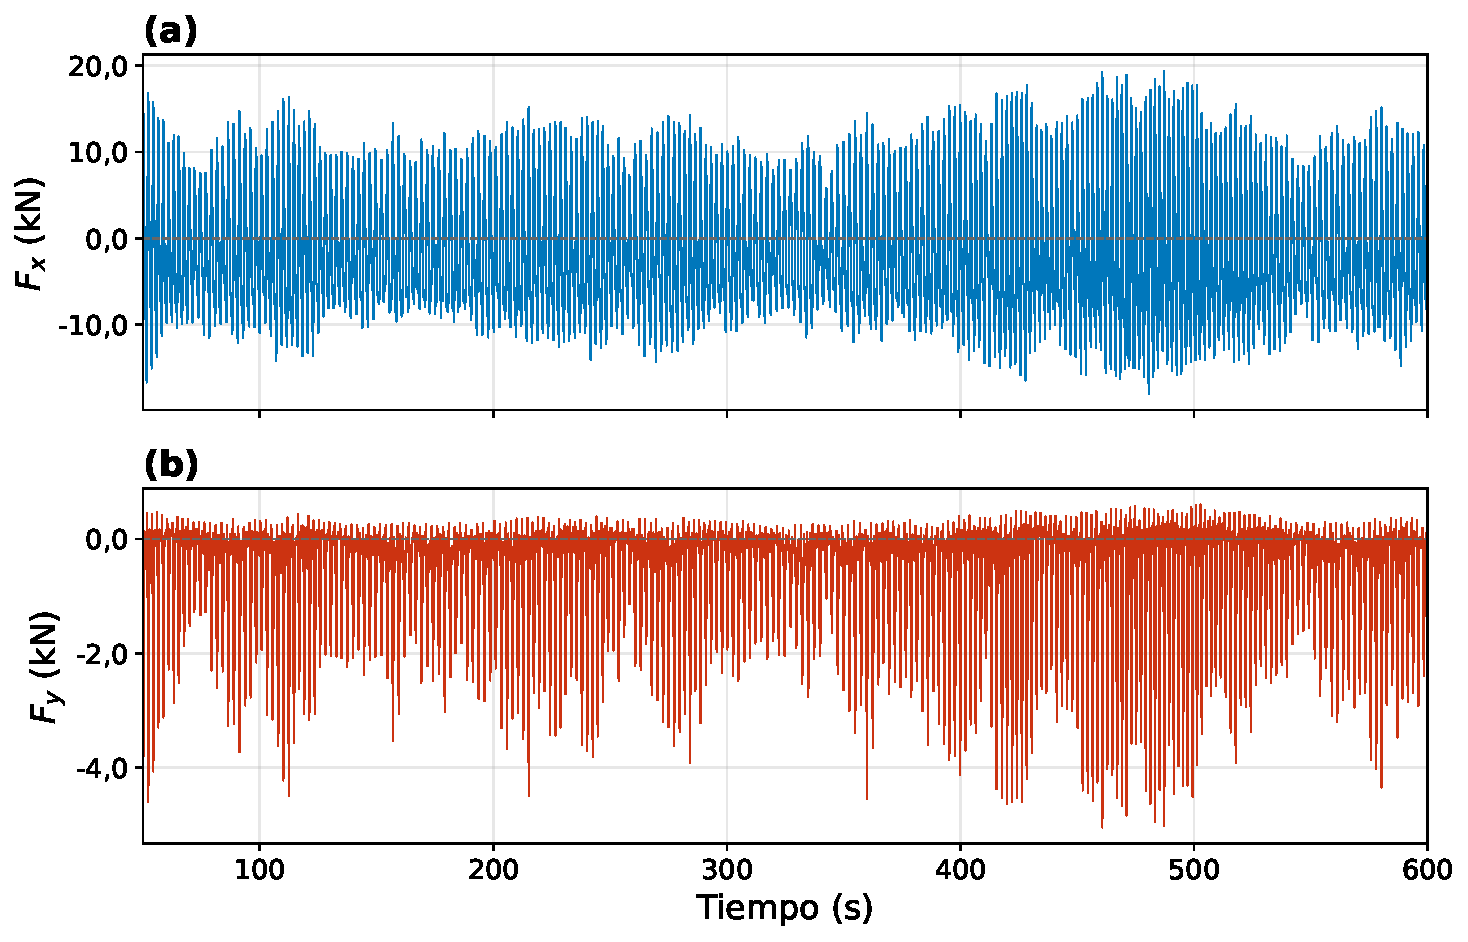
\includegraphics[width=0.85\textwidth]{Figuras/Figuras Anexo Fuerzas/fuerzas_xy_V8_S3.pdf}
    \caption{Fuerzas resultantes (a) $F_x$ y (b) $F_y$ en función del tiempo, $V = 8$~m/s, semilla $3$.}
    \label{fig:anexo_fuerzas_xy_V8_S3}
\end{figure}

\begin{figure}[H]
    \centering
    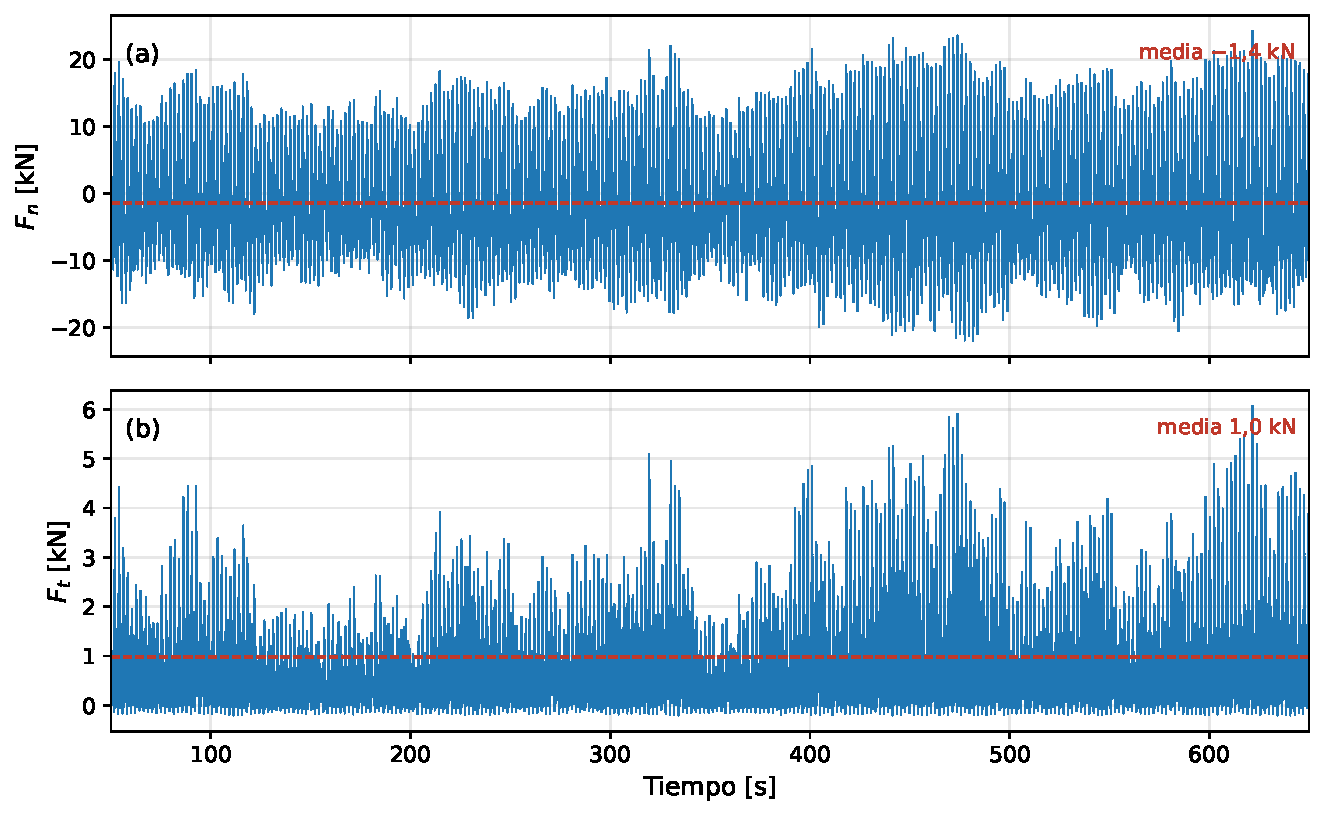
\includegraphics[width=0.85\textwidth]{Figuras/Figuras Anexo Fuerzas/fuerzas_xy_V8_S4.pdf}
    \caption{Fuerzas resultantes (a) $F_x$ y (b) $F_y$ en función del tiempo, $V = 8$~m/s, semilla $4$.}
    \label{fig:anexo_fuerzas_xy_V8_S4}
\end{figure}

\begin{figure}[H]
    \centering
    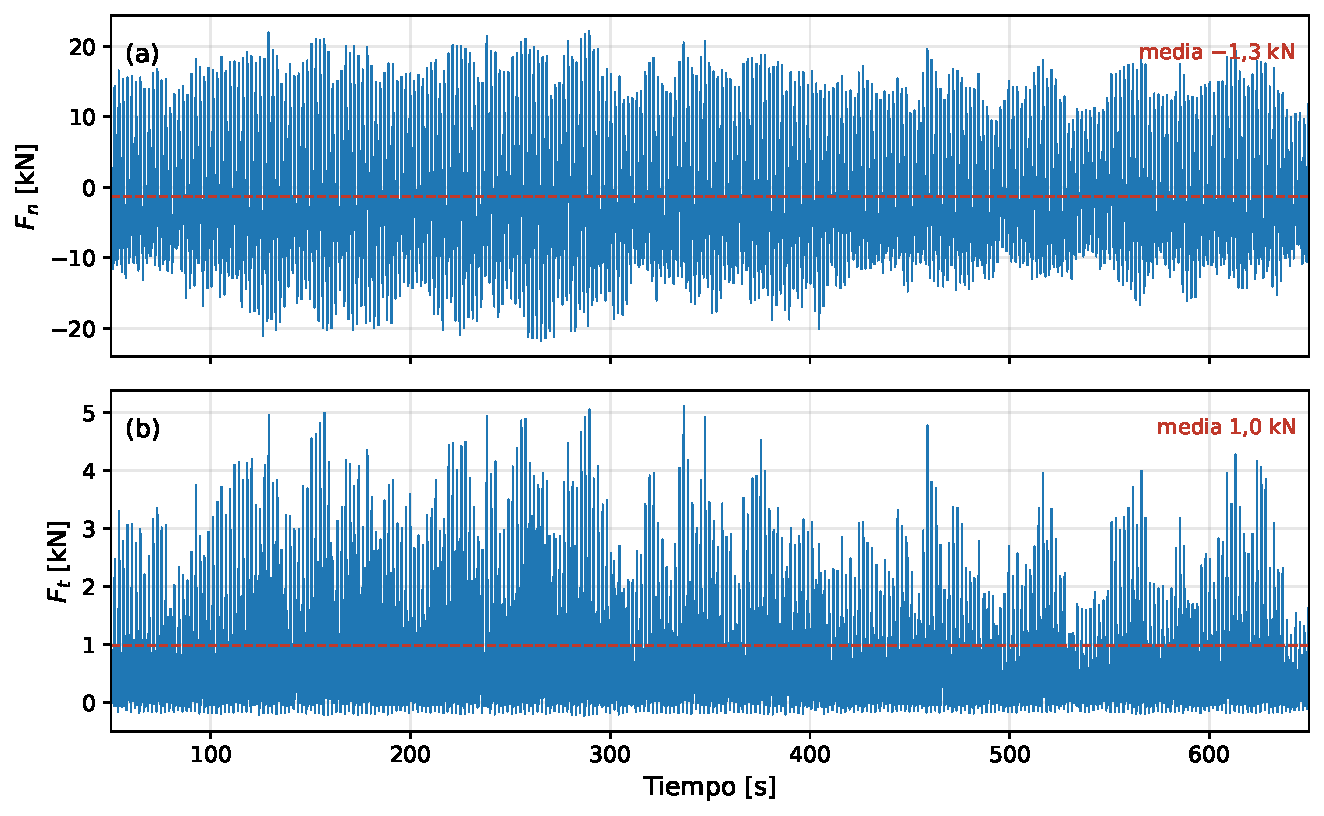
\includegraphics[width=0.85\textwidth]{Figuras/Figuras Anexo Fuerzas/fuerzas_xy_V8_S5.pdf}
    \caption{Fuerzas resultantes (a) $F_x$ y (b) $F_y$ en función del tiempo, $V = 8$~m/s, semilla $5$.}
    \label{fig:anexo_fuerzas_xy_V8_S5}
\end{figure}

\begin{figure}[H]
    \centering
    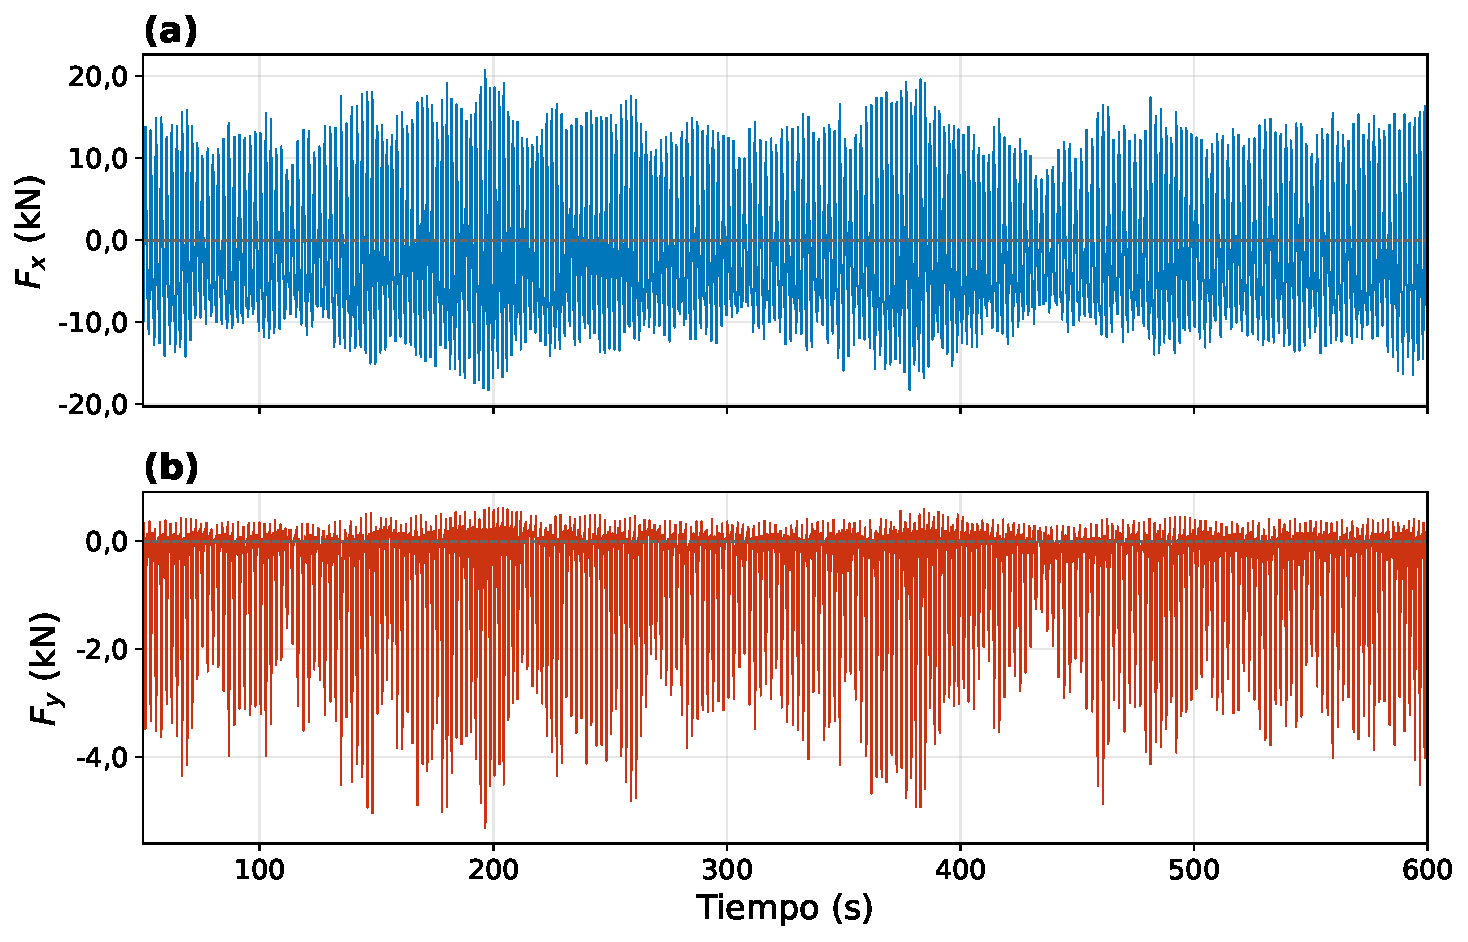
\includegraphics[width=0.85\textwidth]{Figuras/Figuras Anexo Fuerzas/fuerzas_xy_V8_S6.pdf}
    \caption{Fuerzas resultantes (a) $F_x$ y (b) $F_y$ en función del tiempo, $V = 8$~m/s, semilla $6$.}
    \label{fig:anexo_fuerzas_xy_V8_S6}
\end{figure}

\begin{figure}[H]
    \centering
    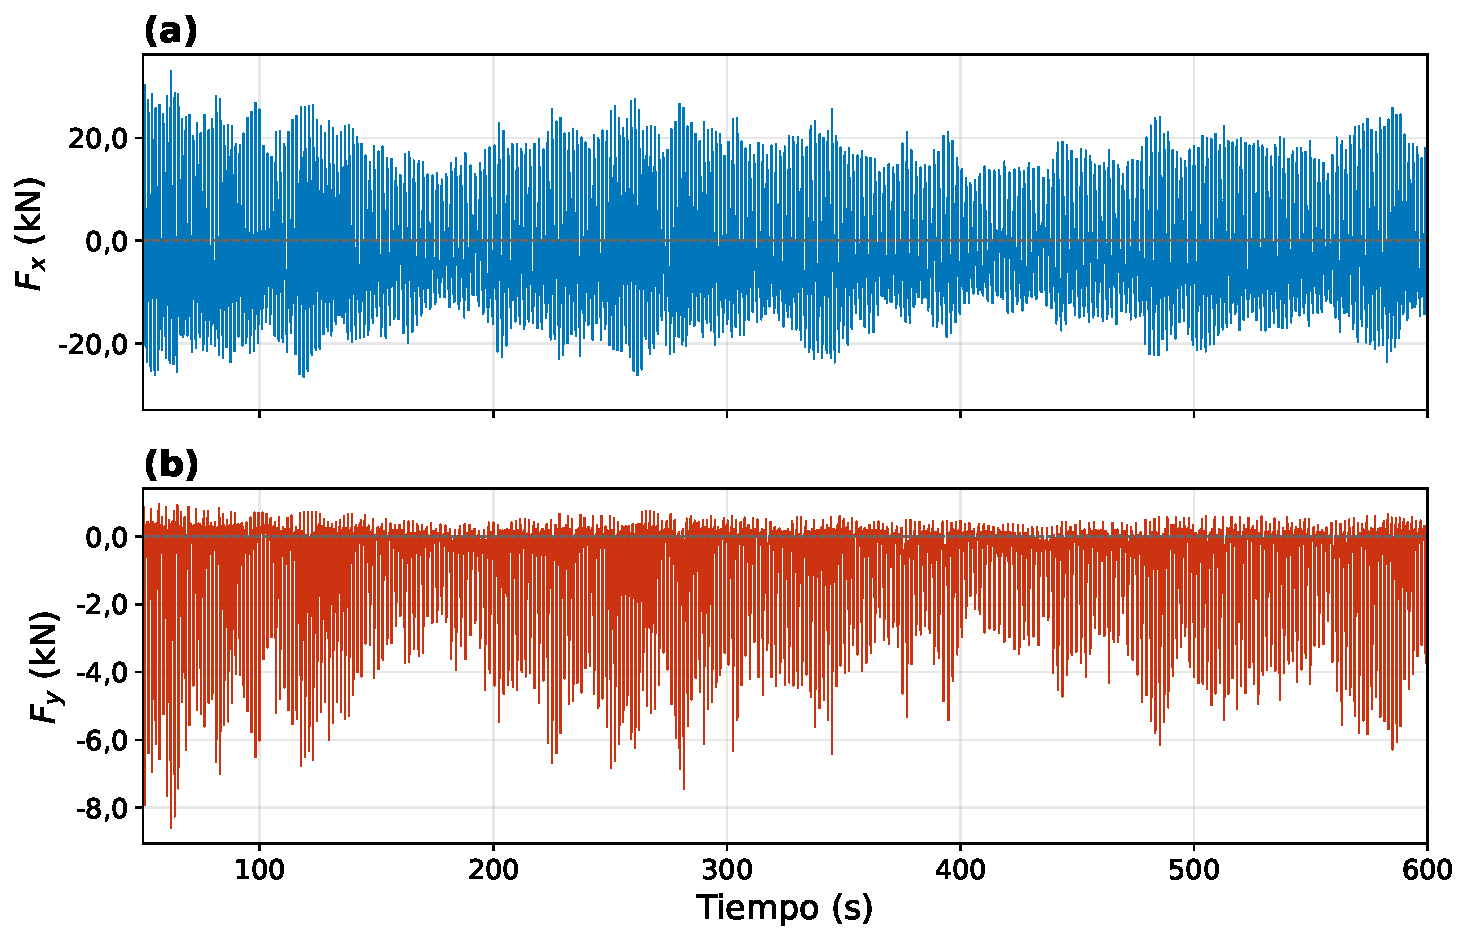
\includegraphics[width=0.85\textwidth]{Figuras/Figuras Anexo Fuerzas/fuerzas_xy_V10_S1.pdf}
    \caption{Fuerzas resultantes (a) $F_x$ y (b) $F_y$ en función del tiempo, $V = 10$~m/s, semilla $1$.}
    \label{fig:anexo_fuerzas_xy_V10_S1}
\end{figure}

\begin{figure}[H]
    \centering
    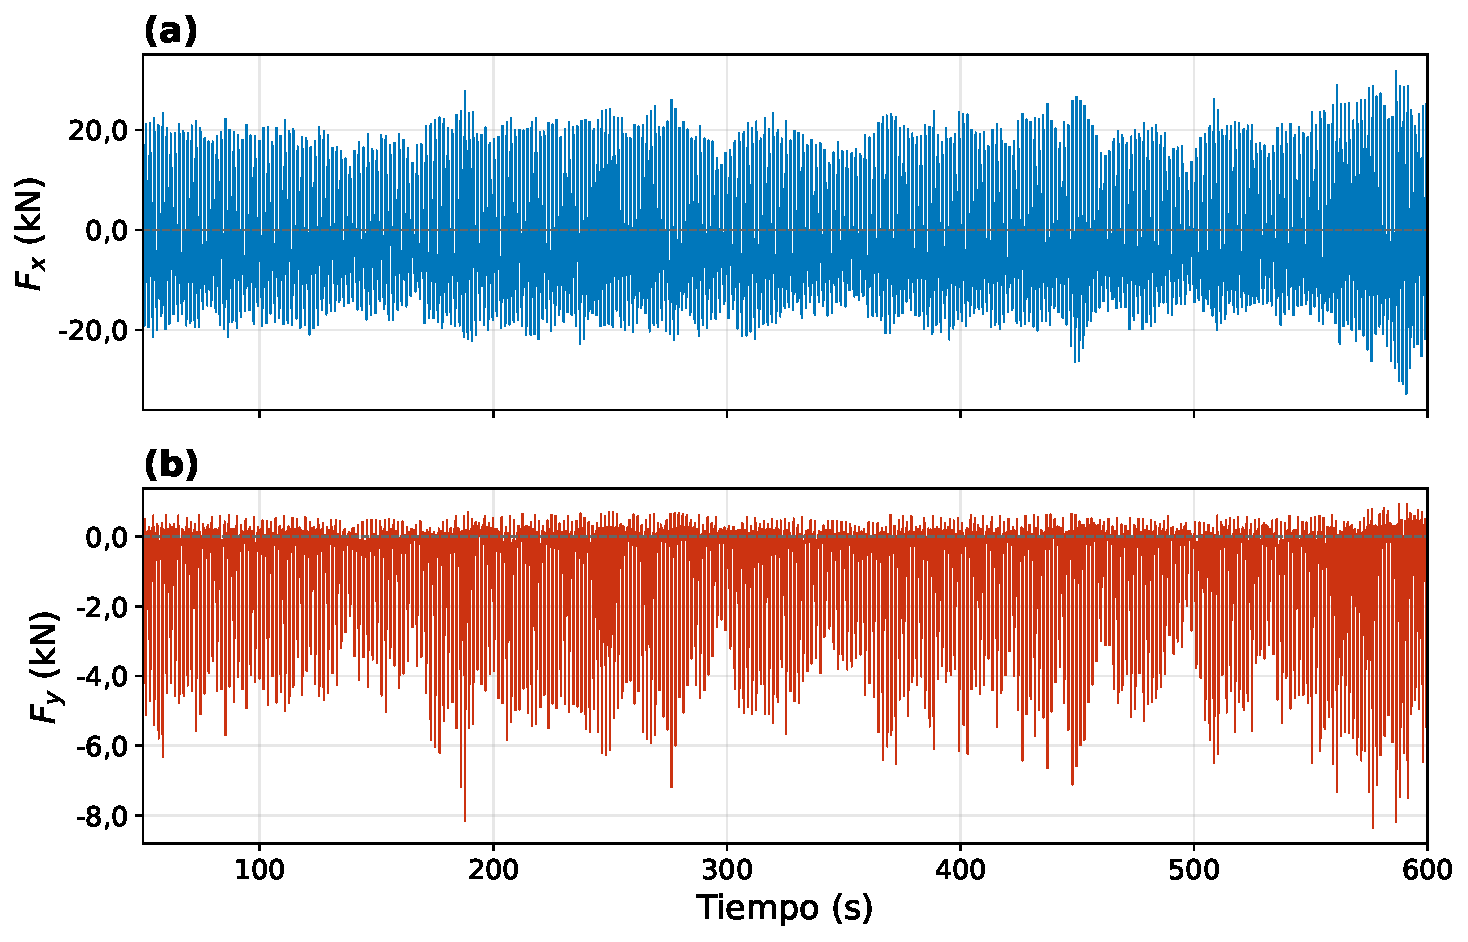
\includegraphics[width=0.85\textwidth]{Figuras/Figuras Anexo Fuerzas/fuerzas_xy_V10_S2.pdf}
    \caption{Fuerzas resultantes (a) $F_x$ y (b) $F_y$ en función del tiempo, $V = 10$~m/s, semilla $2$.}
    \label{fig:anexo_fuerzas_xy_V10_S2}
\end{figure}

\begin{figure}[H]
    \centering
    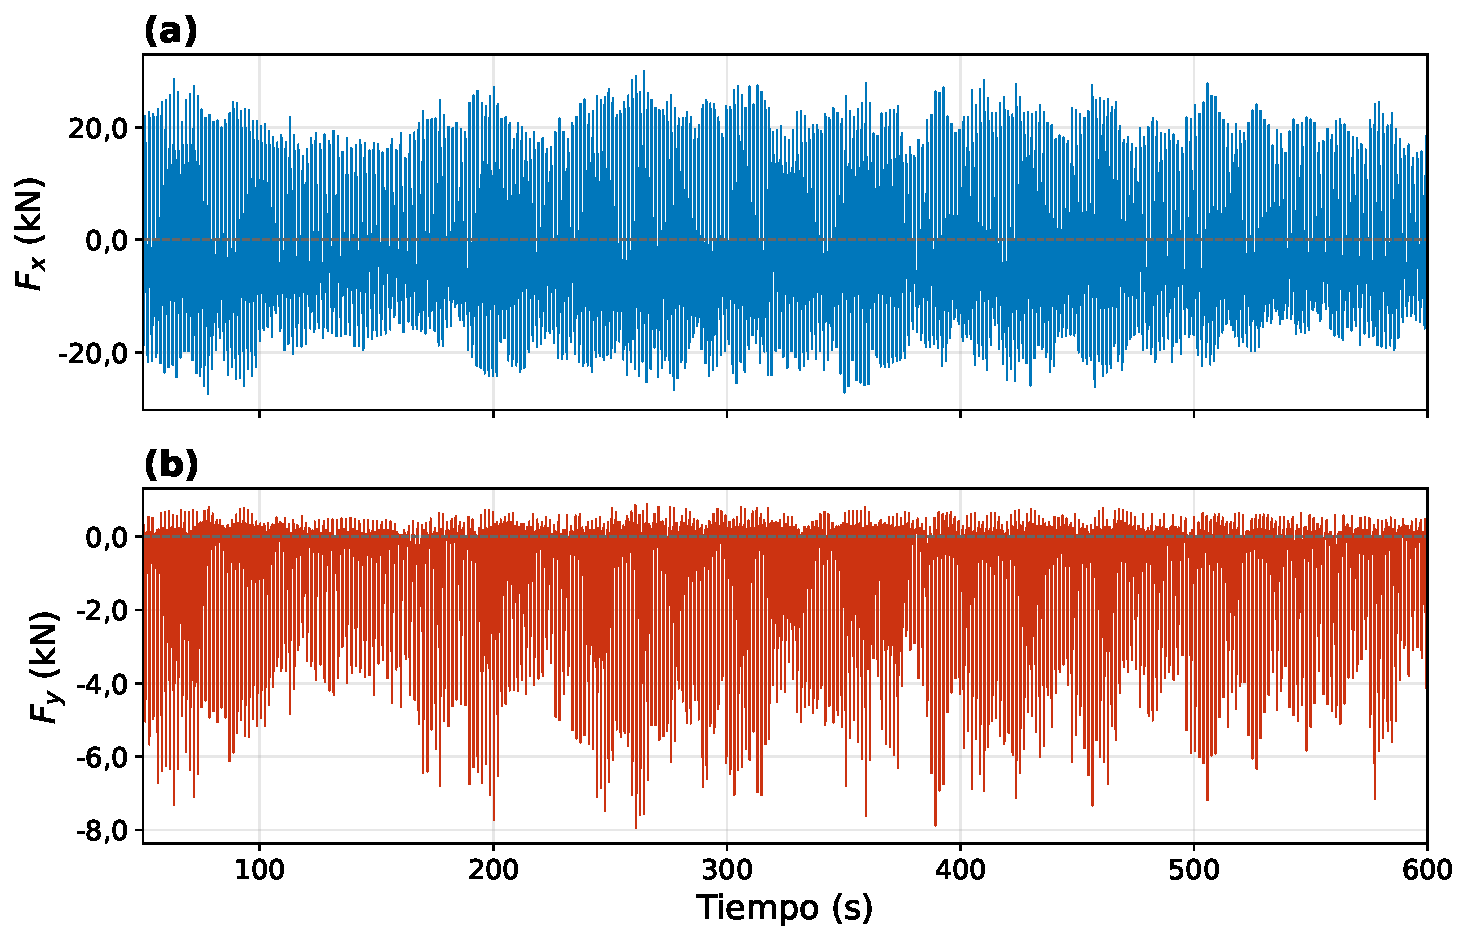
\includegraphics[width=0.85\textwidth]{Figuras/Figuras Anexo Fuerzas/fuerzas_xy_V10_S3.pdf}
    \caption{Fuerzas resultantes (a) $F_x$ y (b) $F_y$ en función del tiempo, $V = 10$~m/s, semilla $3$.}
    \label{fig:anexo_fuerzas_xy_V10_S3}
\end{figure}

\begin{figure}[H]
    \centering
    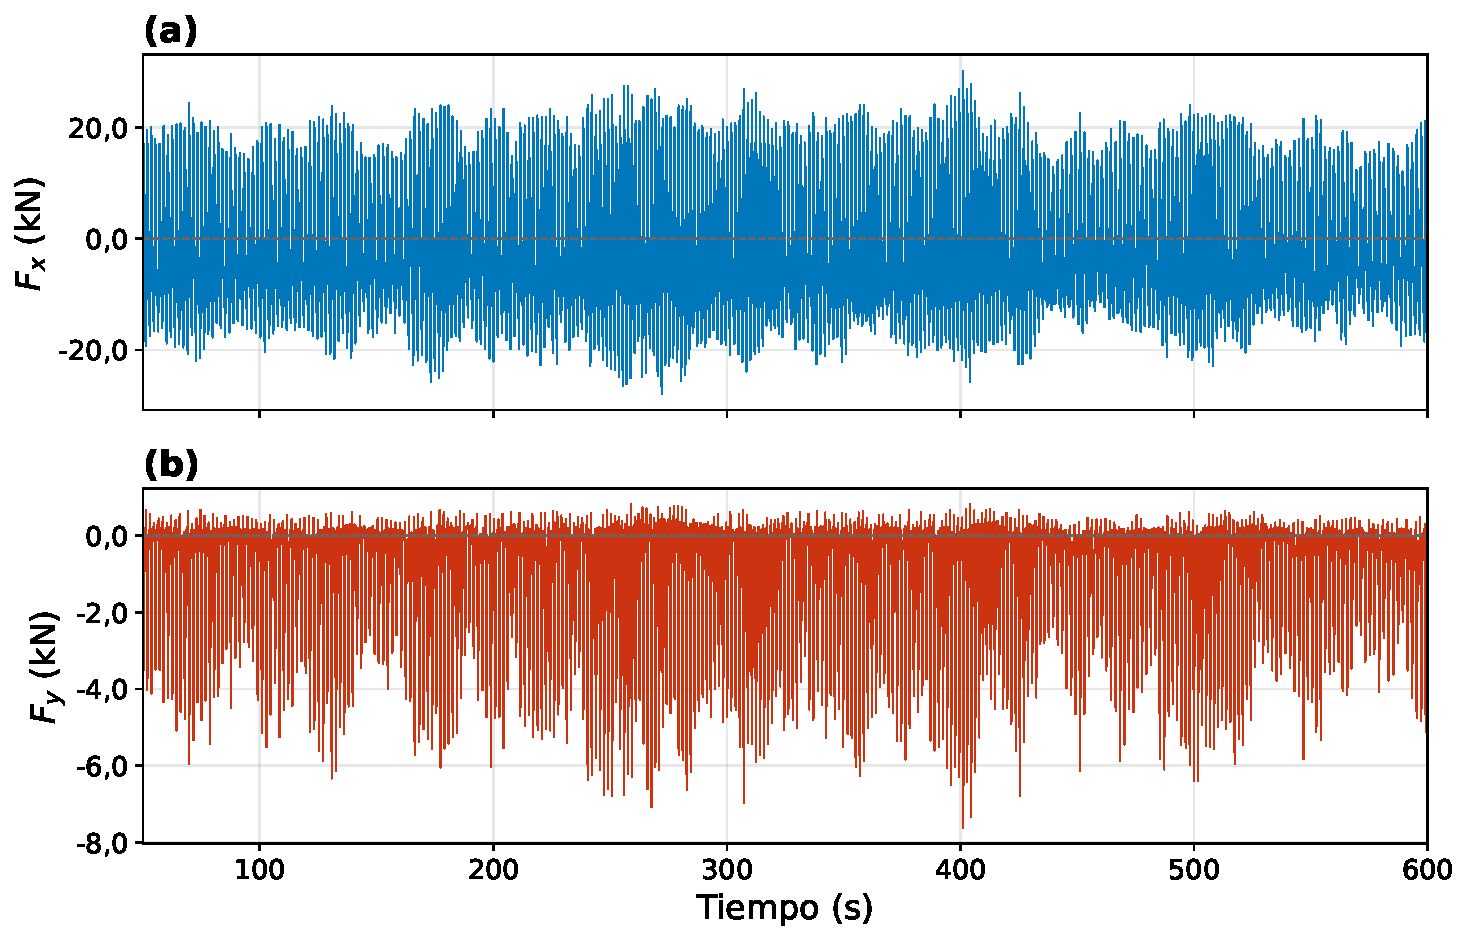
\includegraphics[width=0.85\textwidth]{Figuras/Figuras Anexo Fuerzas/fuerzas_xy_V10_S4.pdf}
    \caption{Fuerzas resultantes (a) $F_x$ y (b) $F_y$ en función del tiempo, $V = 10$~m/s, semilla $4$.}
    \label{fig:anexo_fuerzas_xy_V10_S4}
\end{figure}

\begin{figure}[H]
    \centering
    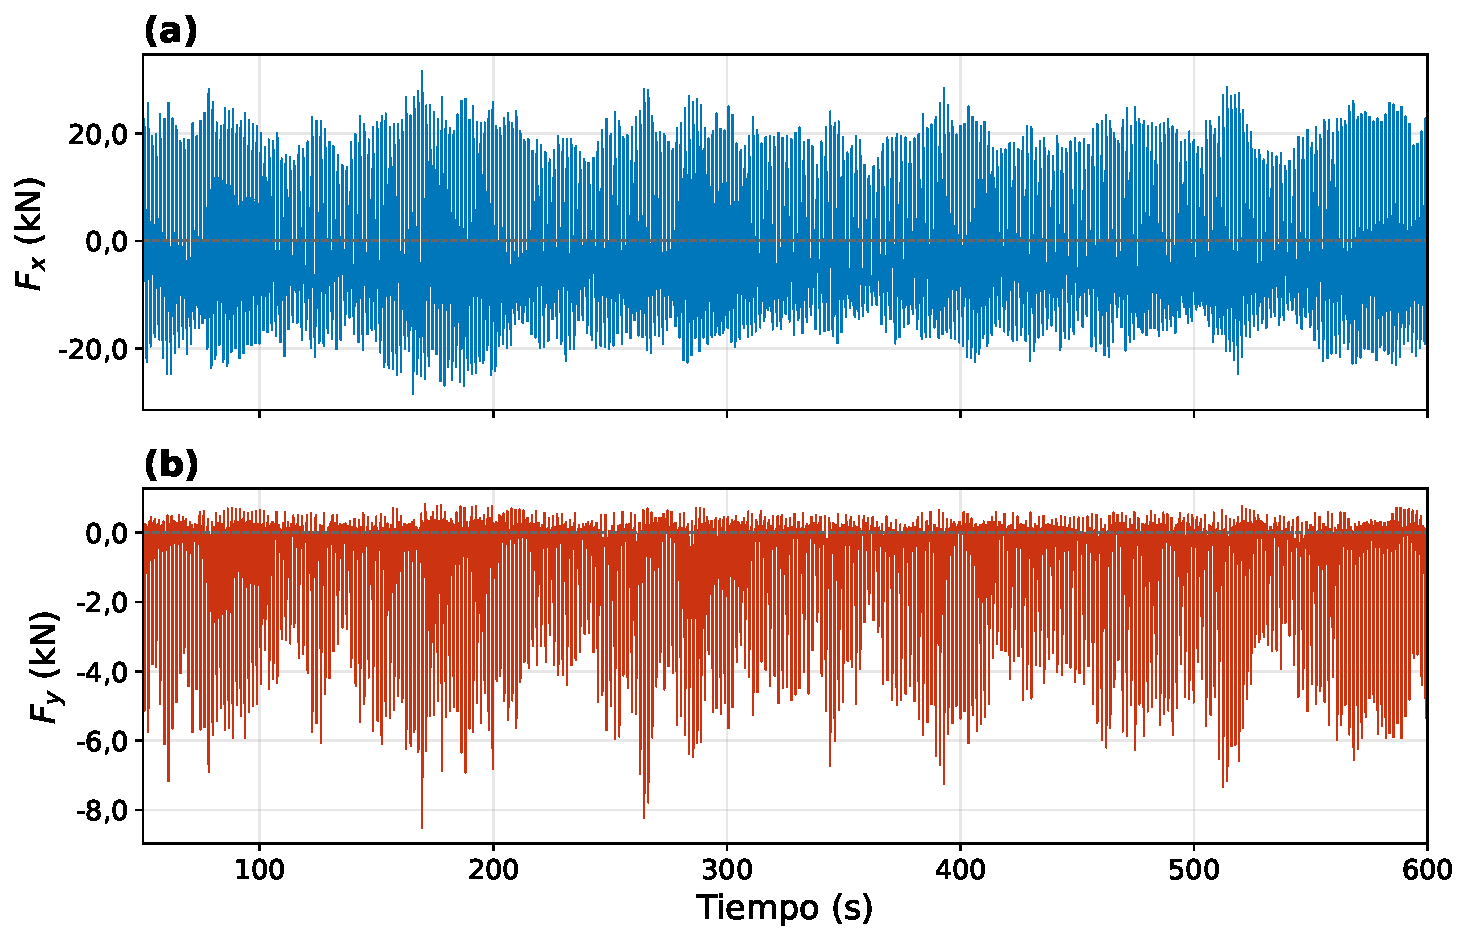
\includegraphics[width=0.85\textwidth]{Figuras/Figuras Anexo Fuerzas/fuerzas_xy_V10_S5.pdf}
    \caption{Fuerzas resultantes (a) $F_x$ y (b) $F_y$ en función del tiempo, $V = 10$~m/s, semilla $5$.}
    \label{fig:anexo_fuerzas_xy_V10_S5}
\end{figure}

\begin{figure}[H]
    \centering
    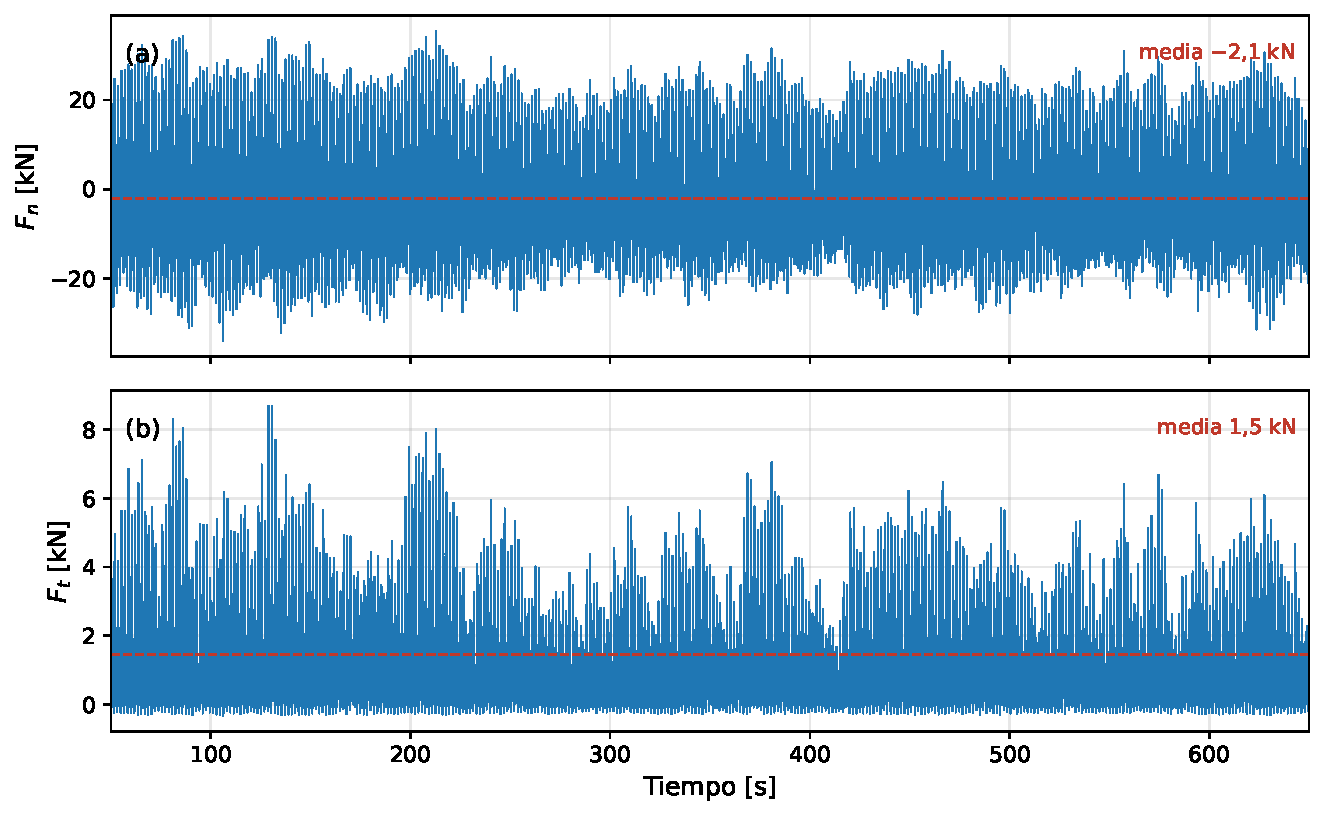
\includegraphics[width=0.85\textwidth]{Figuras/Figuras Anexo Fuerzas/fuerzas_xy_V10_S6.pdf}
    \caption{Fuerzas resultantes (a) $F_x$ y (b) $F_y$ en función del tiempo, $V = 10$~m/s, semilla $6$.}
    \label{fig:anexo_fuerzas_xy_V10_S6}
\end{figure}

\begin{figure}[H]
    \centering
    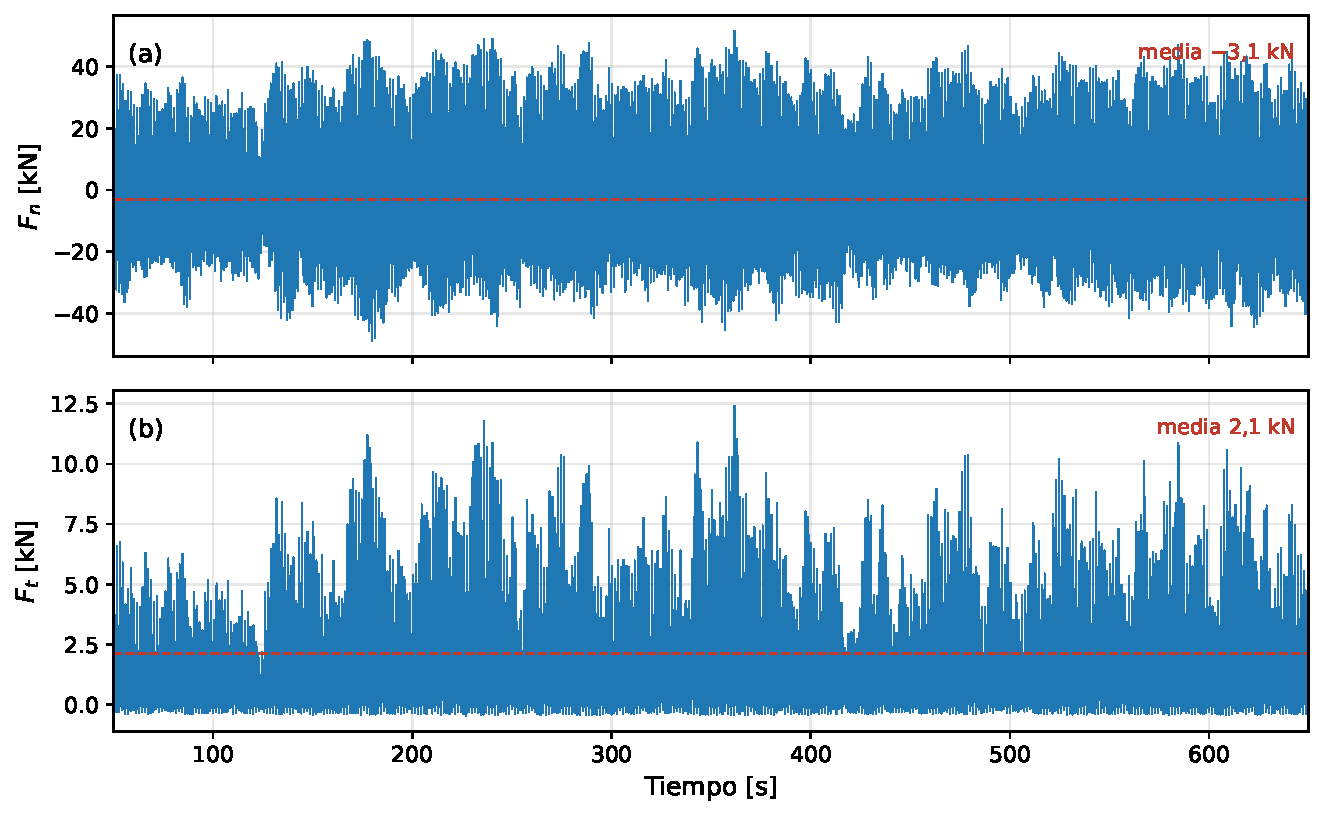
\includegraphics[width=0.85\textwidth]{Figuras/Figuras Anexo Fuerzas/fuerzas_xy_V12_S1.pdf}
    \caption{Fuerzas resultantes (a) $F_x$ y (b) $F_y$ en función del tiempo, $V = 12$~m/s, semilla $1$.}
    \label{fig:anexo_fuerzas_xy_V12_S1}
\end{figure}

\begin{figure}[H]
    \centering
    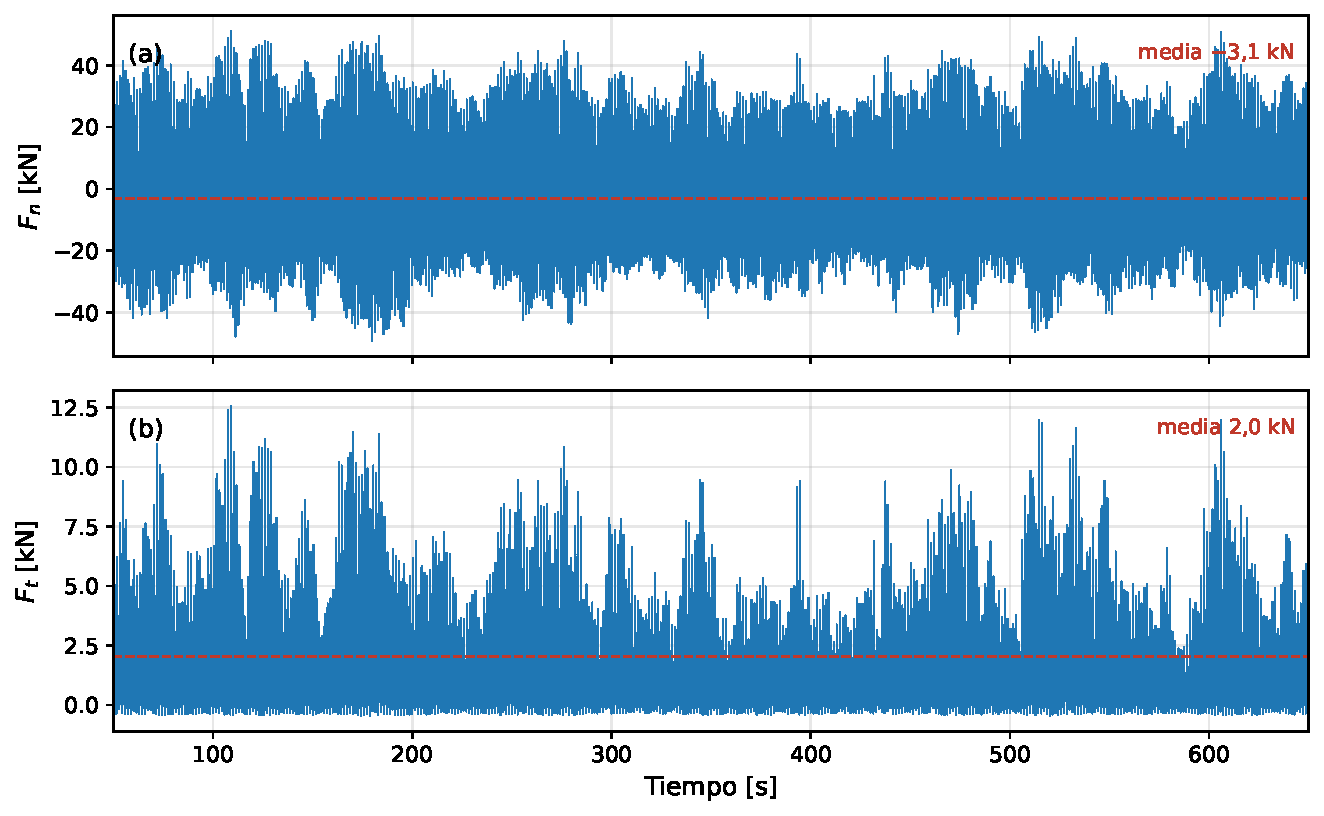
\includegraphics[width=0.85\textwidth]{Figuras/Figuras Anexo Fuerzas/fuerzas_xy_V12_S2.pdf}
    \caption{Fuerzas resultantes (a) $F_x$ y (b) $F_y$ en función del tiempo, $V = 12$~m/s, semilla $2$.}
    \label{fig:anexo_fuerzas_xy_V12_S2}
\end{figure}

\begin{figure}[H]
    \centering
    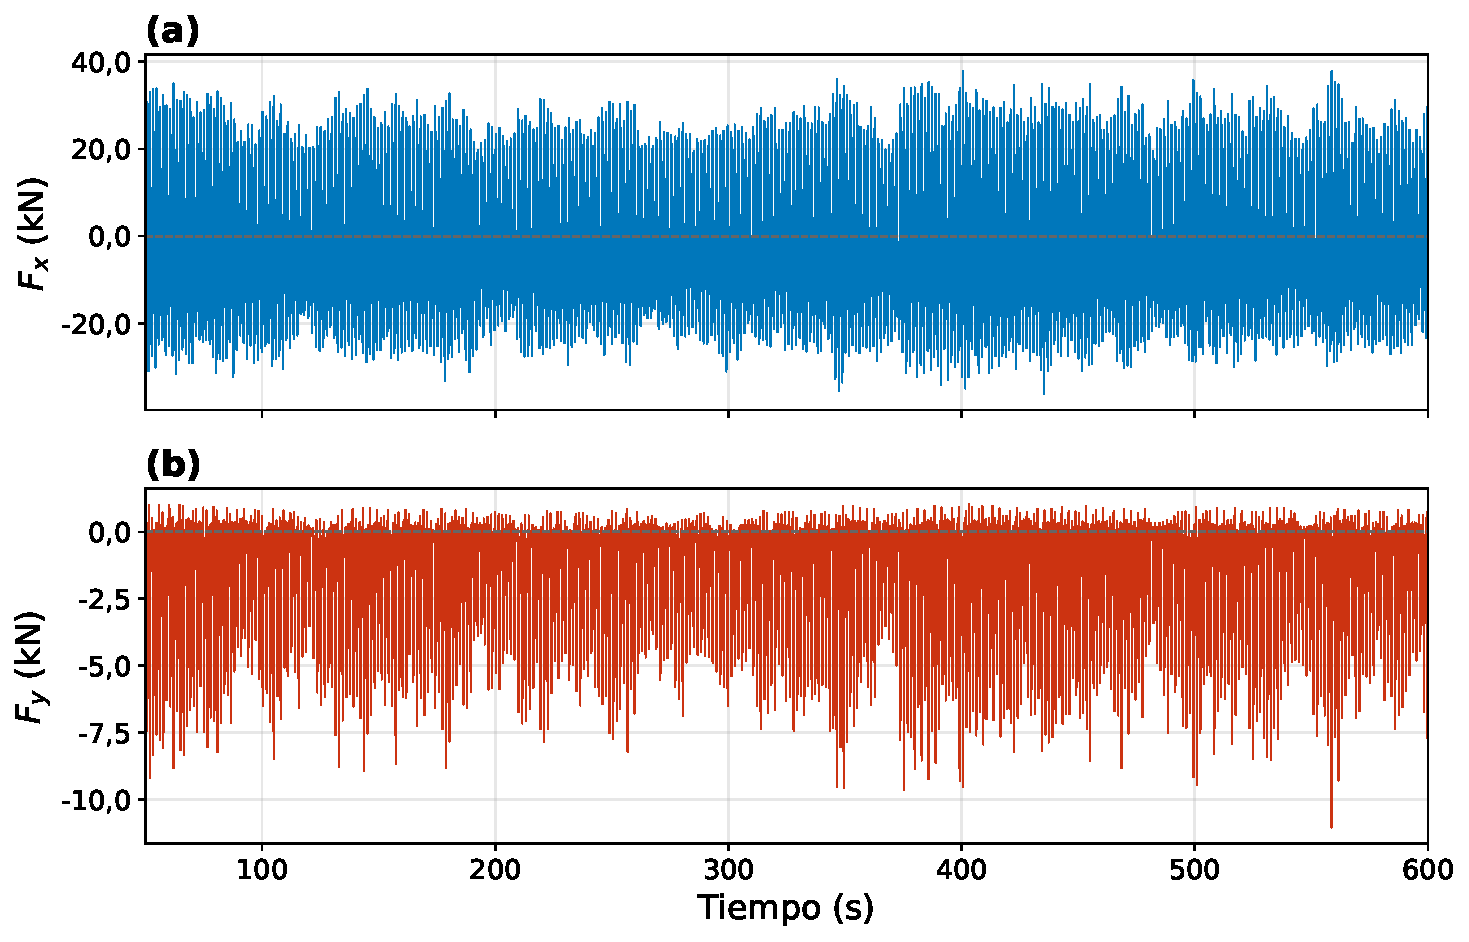
\includegraphics[width=0.85\textwidth]{Figuras/Figuras Anexo Fuerzas/fuerzas_xy_V12_S3.pdf}
    \caption{Fuerzas resultantes (a) $F_x$ y (b) $F_y$ en función del tiempo, $V = 12$~m/s, semilla $3$.}
    \label{fig:anexo_fuerzas_xy_V12_S3}
\end{figure}

\begin{figure}[H]
    \centering
    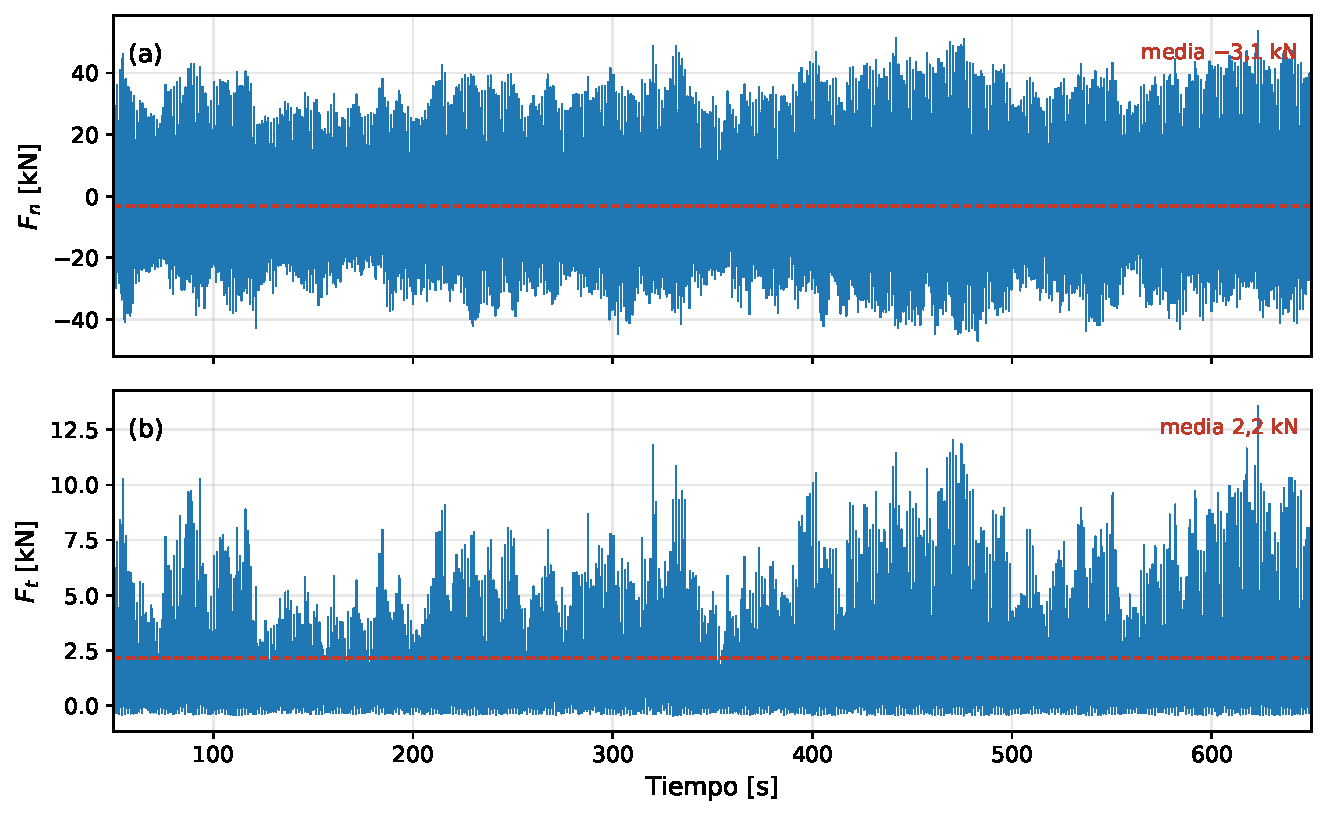
\includegraphics[width=0.85\textwidth]{Figuras/Figuras Anexo Fuerzas/fuerzas_xy_V12_S4.pdf}
    \caption{Fuerzas resultantes (a) $F_x$ y (b) $F_y$ en función del tiempo, $V = 12$~m/s, semilla $4$.}
    \label{fig:anexo_fuerzas_xy_V12_S4}
\end{figure}

\begin{figure}[H]
    \centering
    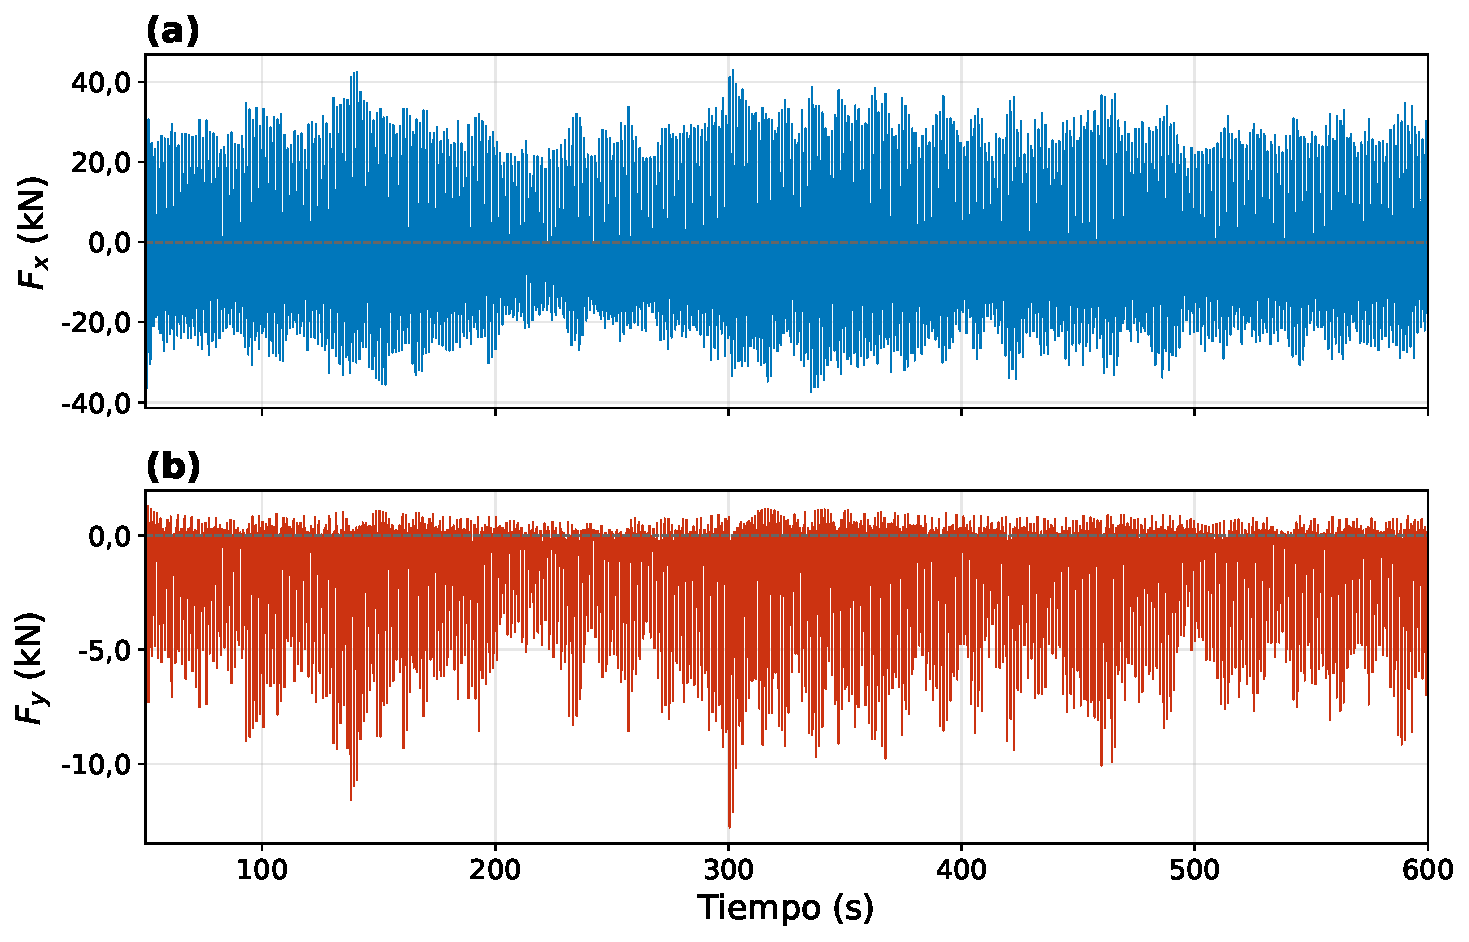
\includegraphics[width=0.85\textwidth]{Figuras/Figuras Anexo Fuerzas/fuerzas_xy_V12_S5.pdf}
    \caption{Fuerzas resultantes (a) $F_x$ y (b) $F_y$ en función del tiempo, $V = 12$~m/s, semilla $5$.}
    \label{fig:anexo_fuerzas_xy_V12_S5}
\end{figure}

\begin{figure}[H]
    \centering
    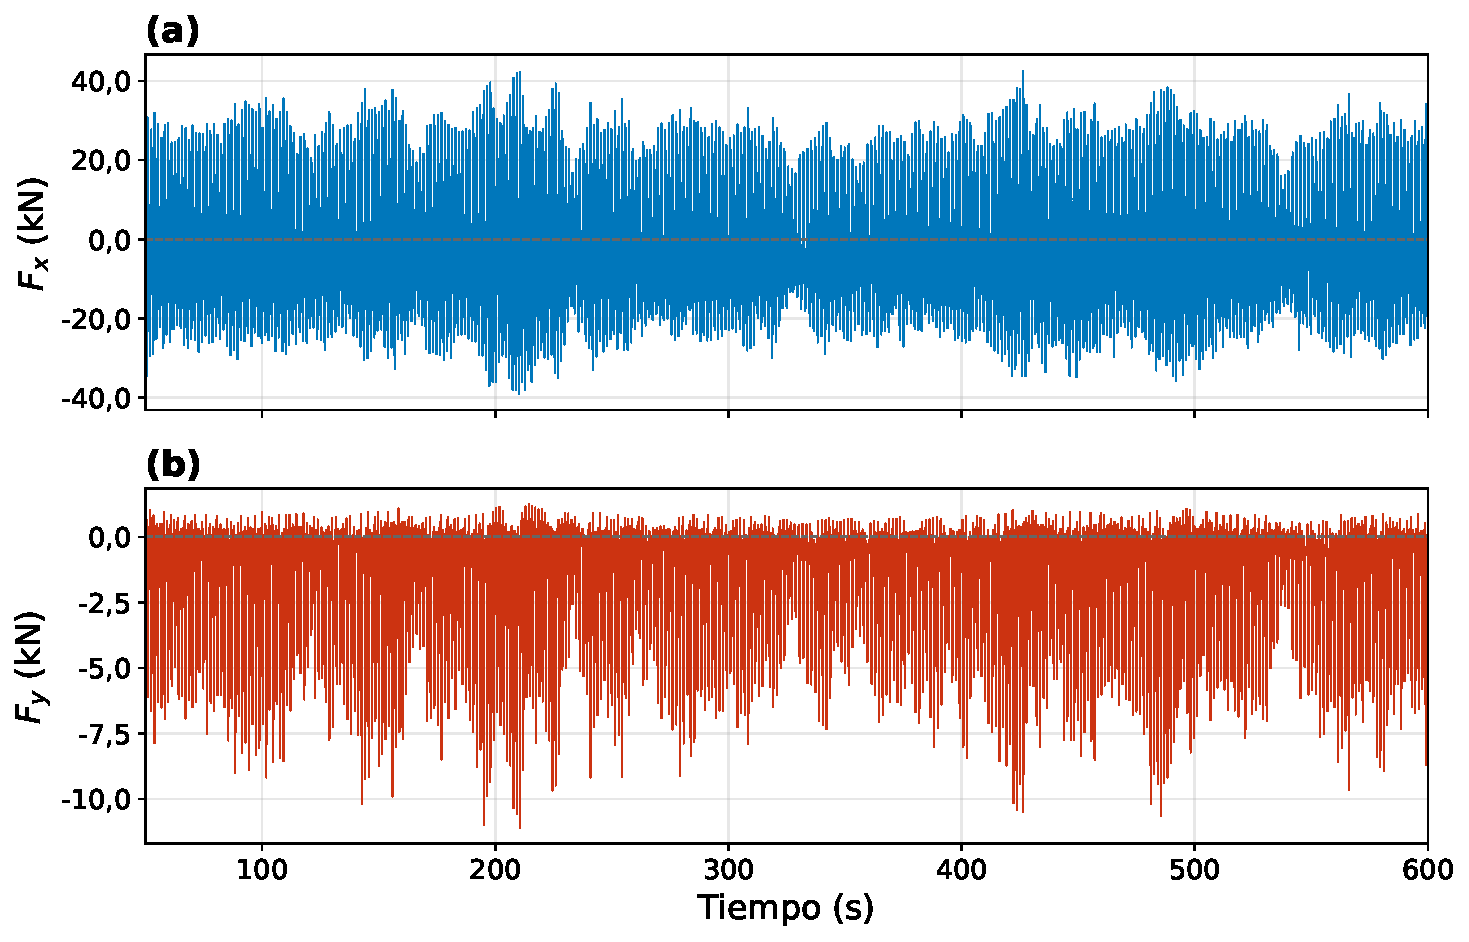
\includegraphics[width=0.85\textwidth]{Figuras/Figuras Anexo Fuerzas/fuerzas_xy_V12_S6.pdf}
    \caption{Fuerzas resultantes (a) $F_x$ y (b) $F_y$ en función del tiempo, $V = 12$~m/s, semilla $6$.}
    \label{fig:anexo_fuerzas_xy_V12_S6}
\end{figure}

\begin{figure}[H]
    \centering
    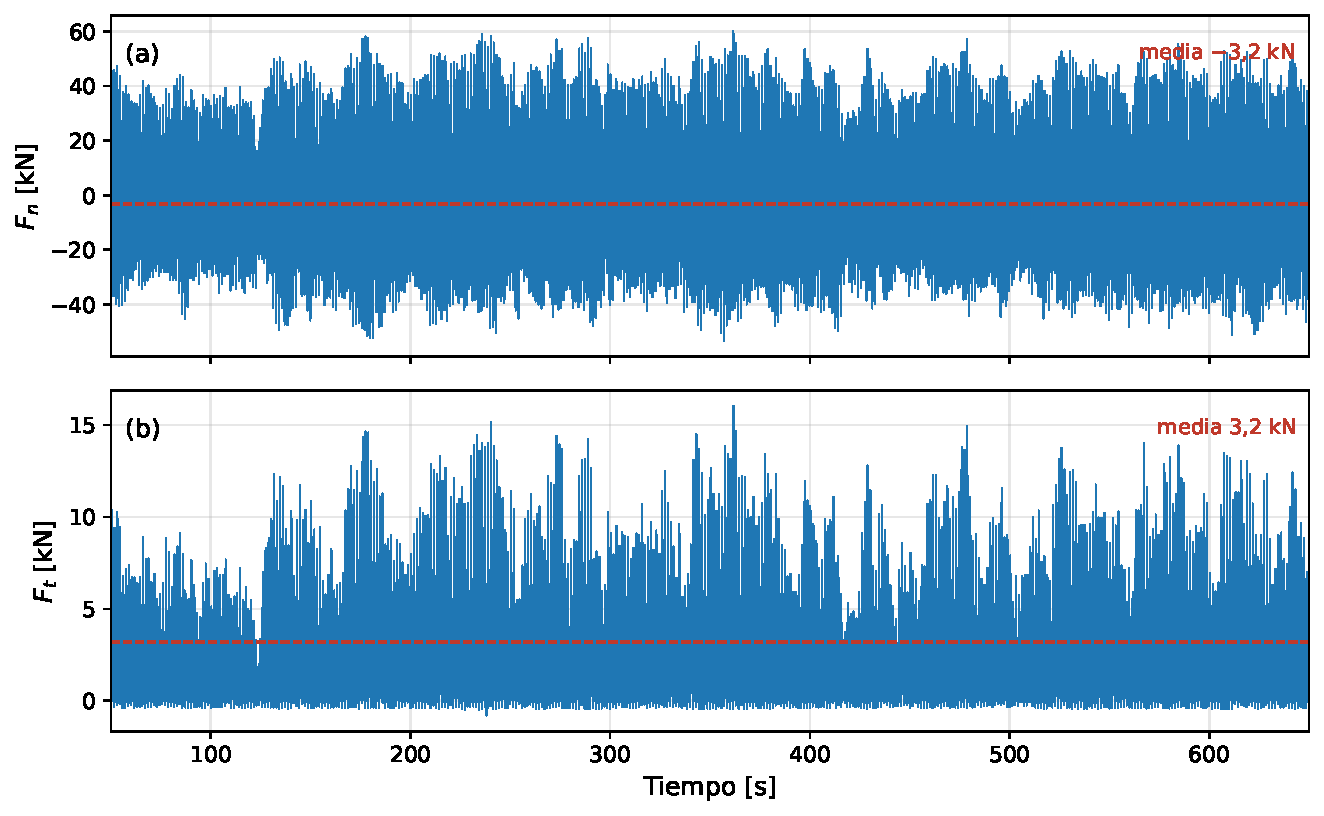
\includegraphics[width=0.85\textwidth]{Figuras/Figuras Anexo Fuerzas/fuerzas_xy_V14_S1.pdf}
    \caption{Fuerzas resultantes (a) $F_x$ y (b) $F_y$ en función del tiempo, $V = 14$~m/s, semilla $1$.}
    \label{fig:anexo_fuerzas_xy_V14_S1}
\end{figure}

\begin{figure}[H]
    \centering
    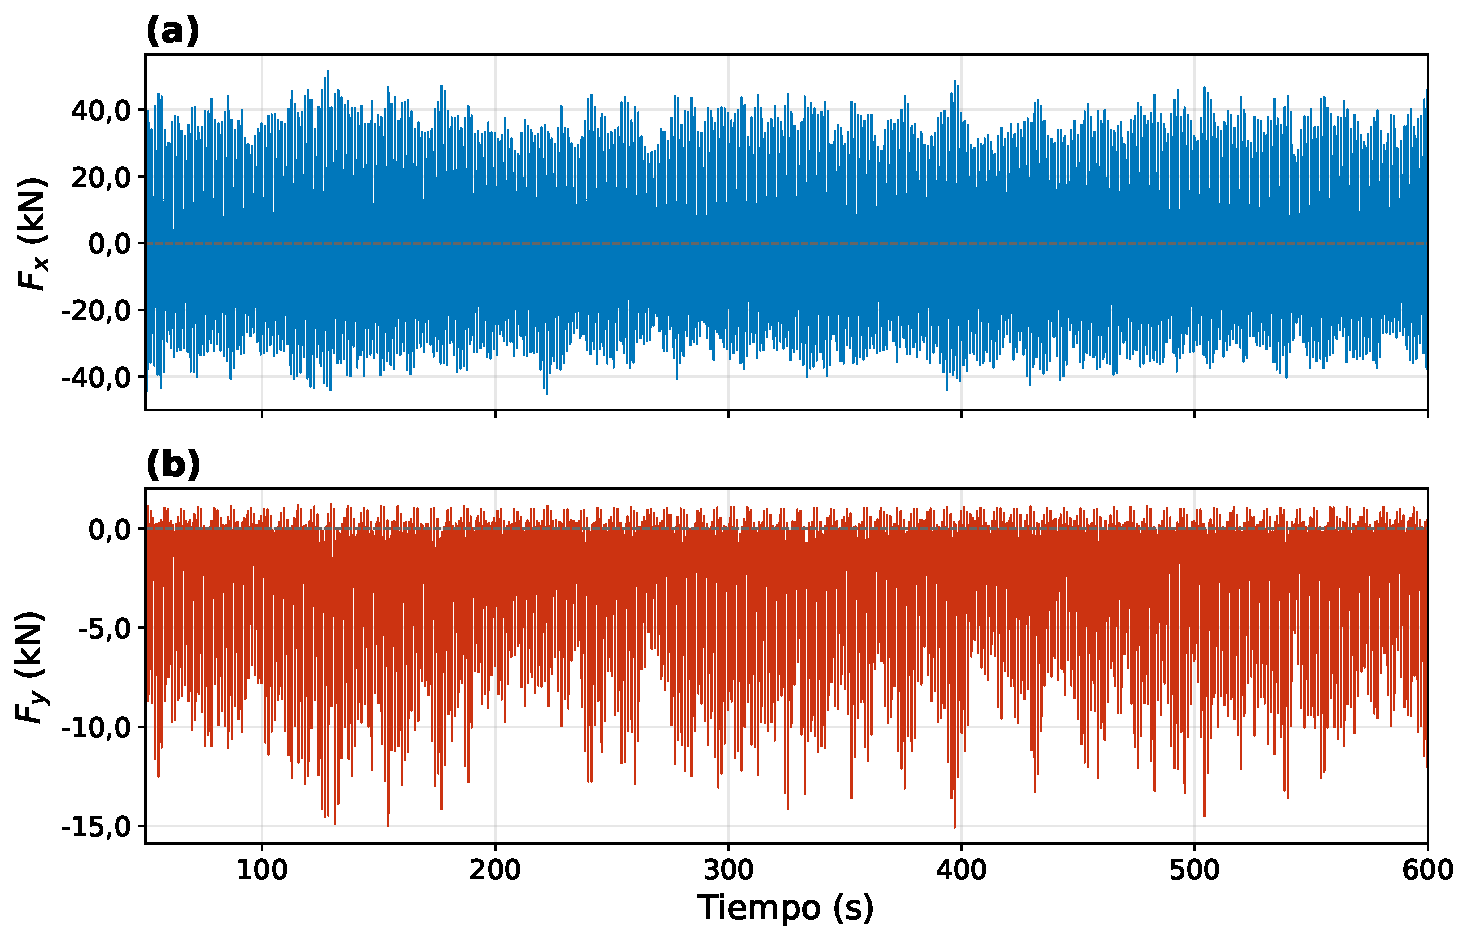
\includegraphics[width=0.85\textwidth]{Figuras/Figuras Anexo Fuerzas/fuerzas_xy_V14_S2.pdf}
    \caption{Fuerzas resultantes (a) $F_x$ y (b) $F_y$ en función del tiempo, $V = 14$~m/s, semilla $2$.}
    \label{fig:anexo_fuerzas_xy_V14_S2}
\end{figure}

\begin{figure}[H]
    \centering
    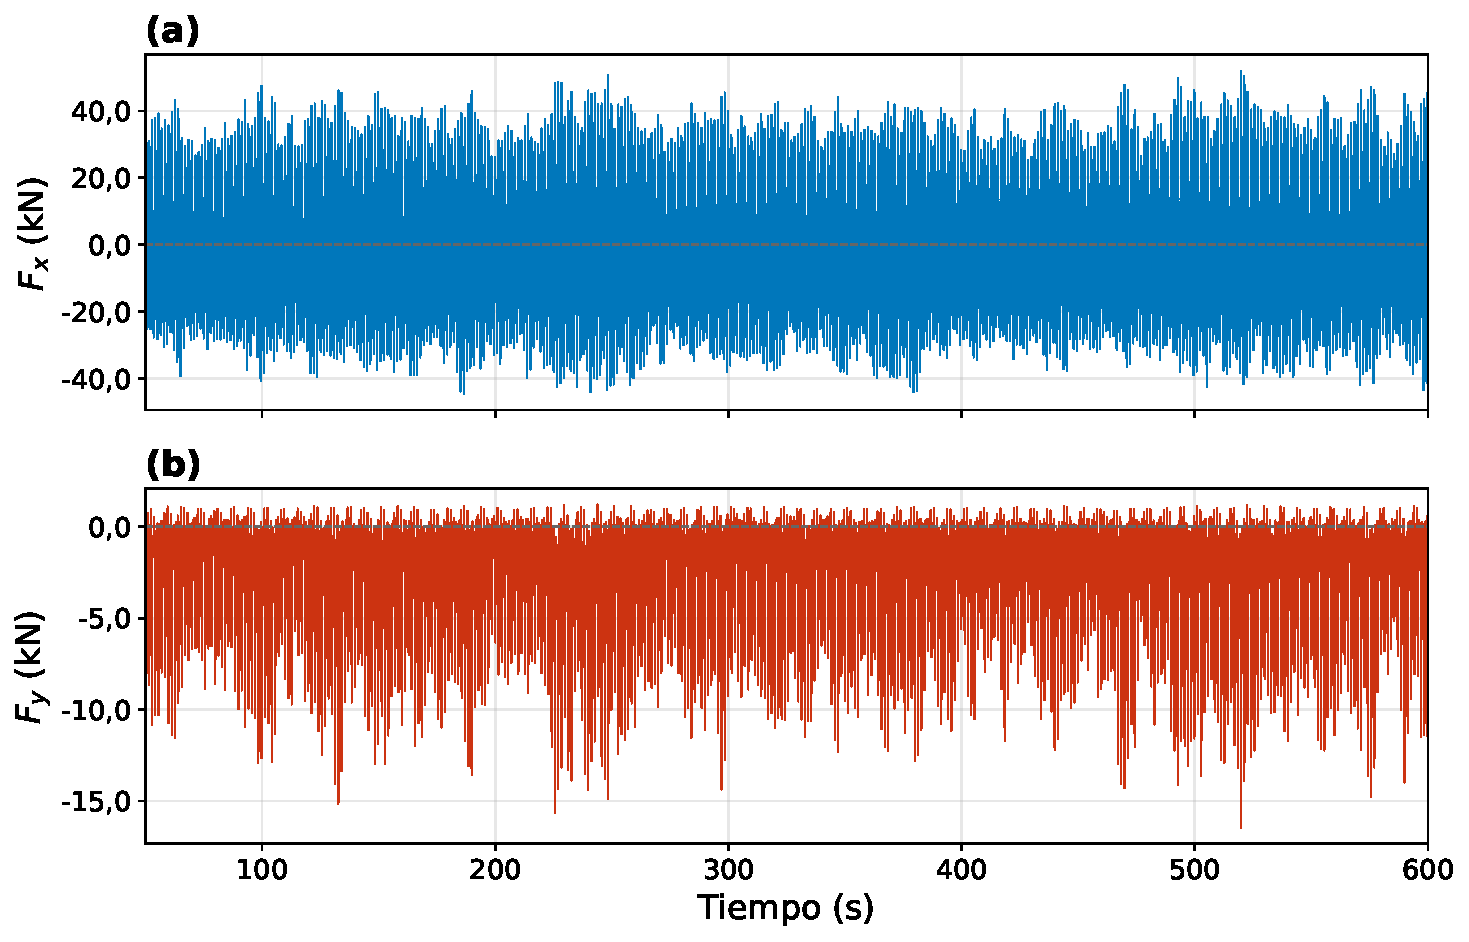
\includegraphics[width=0.85\textwidth]{Figuras/Figuras Anexo Fuerzas/fuerzas_xy_V14_S3.pdf}
    \caption{Fuerzas resultantes (a) $F_x$ y (b) $F_y$ en función del tiempo, $V = 14$~m/s, semilla $3$.}
    \label{fig:anexo_fuerzas_xy_V14_S3}
\end{figure}

\begin{figure}[H]
    \centering
    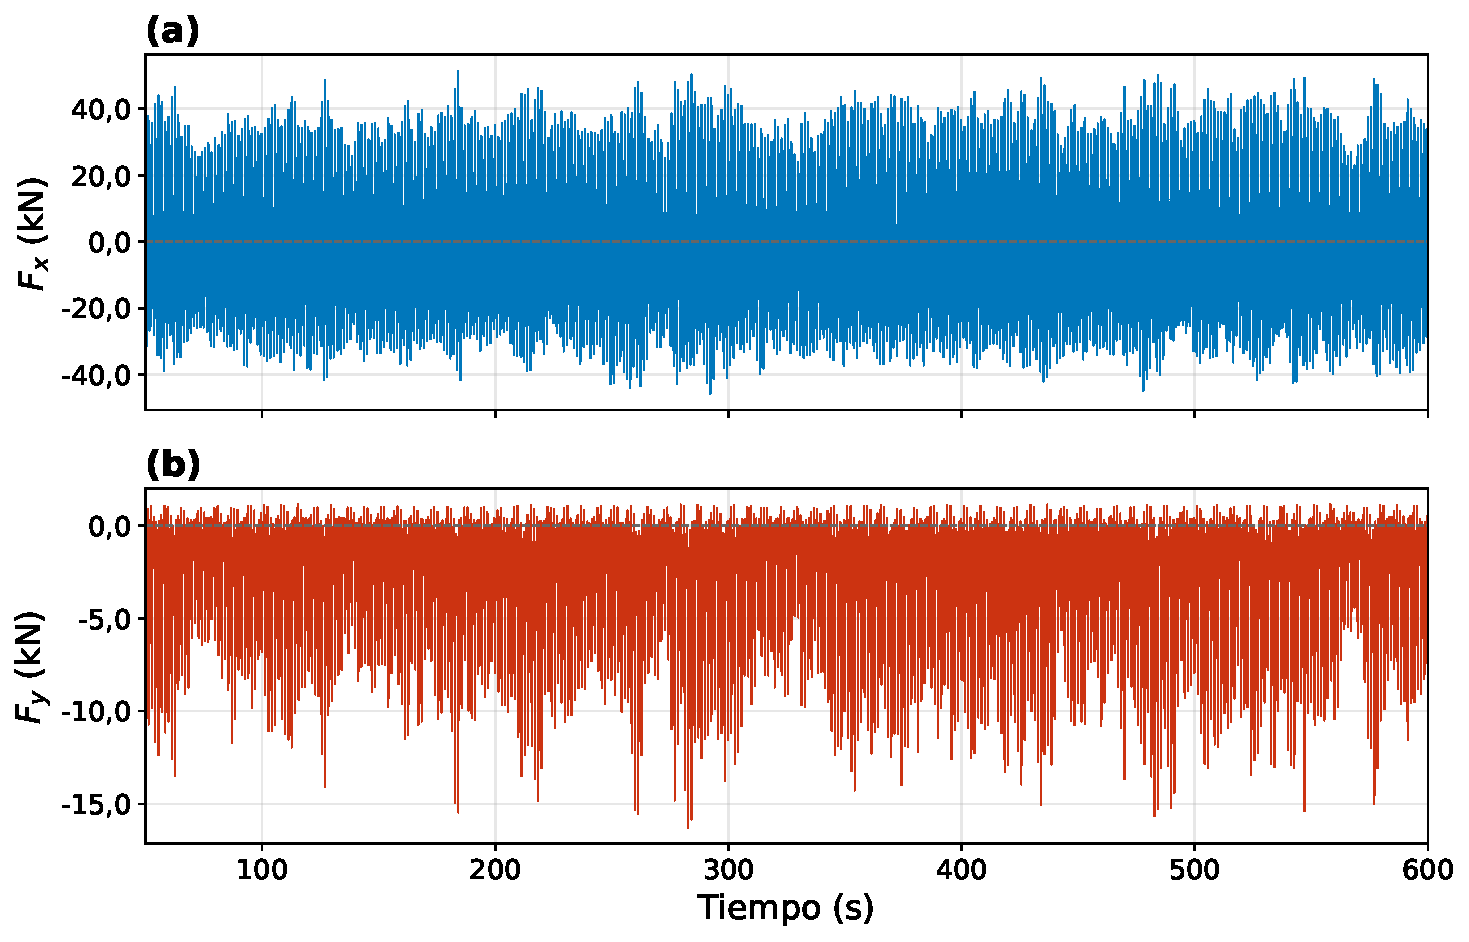
\includegraphics[width=0.85\textwidth]{Figuras/Figuras Anexo Fuerzas/fuerzas_xy_V14_S4.pdf}
    \caption{Fuerzas resultantes (a) $F_x$ y (b) $F_y$ en función del tiempo, $V = 14$~m/s, semilla $4$.}
    \label{fig:anexo_fuerzas_xy_V14_S4}
\end{figure}

\begin{figure}[H]
    \centering
    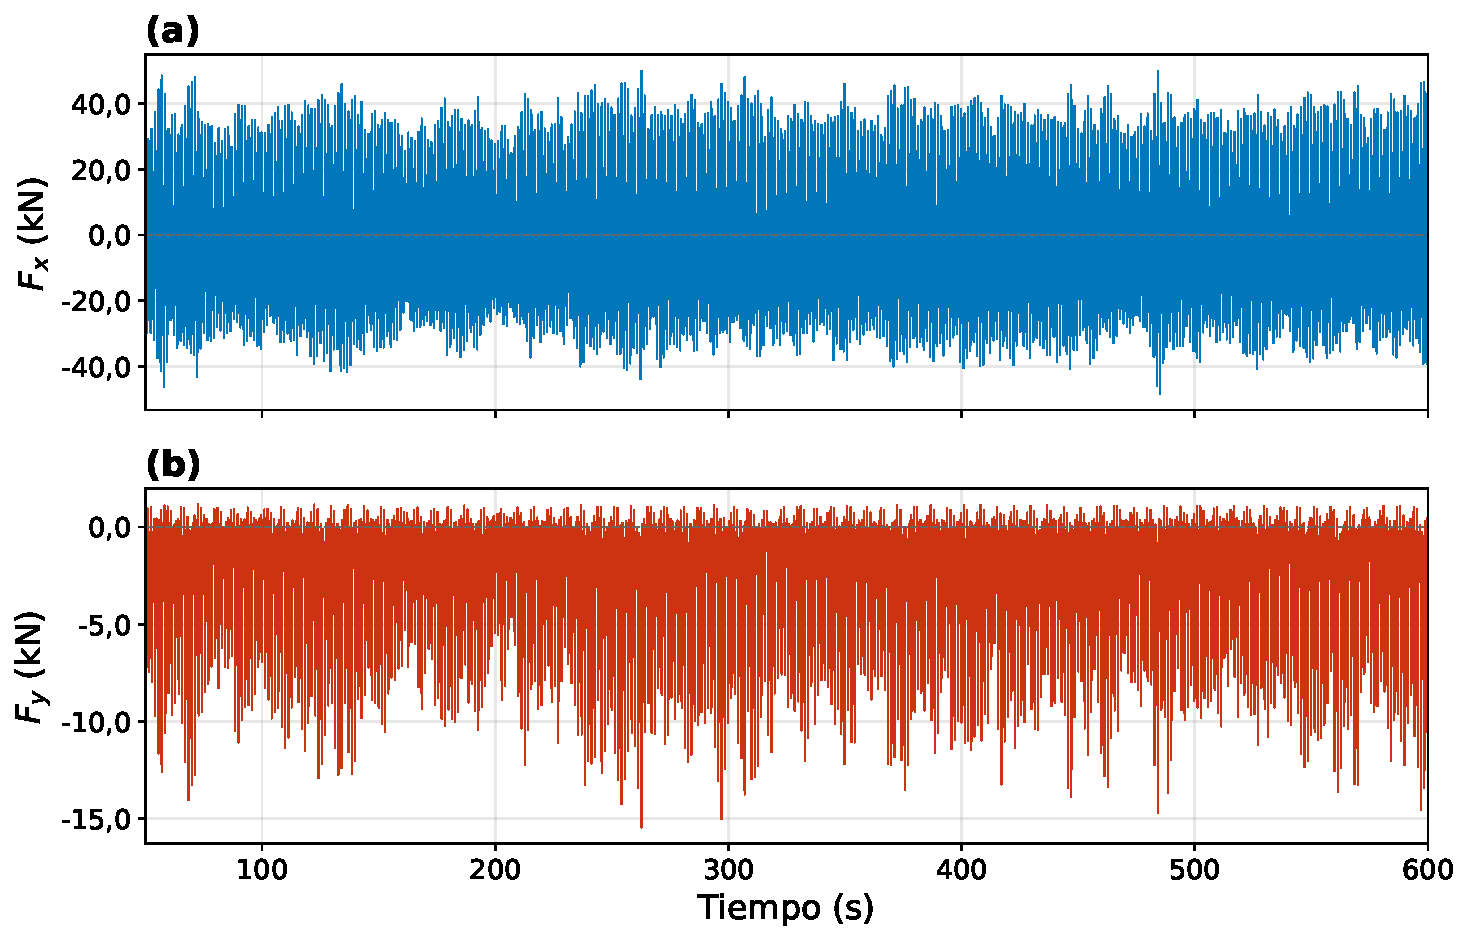
\includegraphics[width=0.85\textwidth]{Figuras/Figuras Anexo Fuerzas/fuerzas_xy_V14_S5.pdf}
    \caption{Fuerzas resultantes (a) $F_x$ y (b) $F_y$ en función del tiempo, $V = 14$~m/s, semilla $5$.}
    \label{fig:anexo_fuerzas_xy_V14_S5}
\end{figure}

\begin{figure}[H]
    \centering
    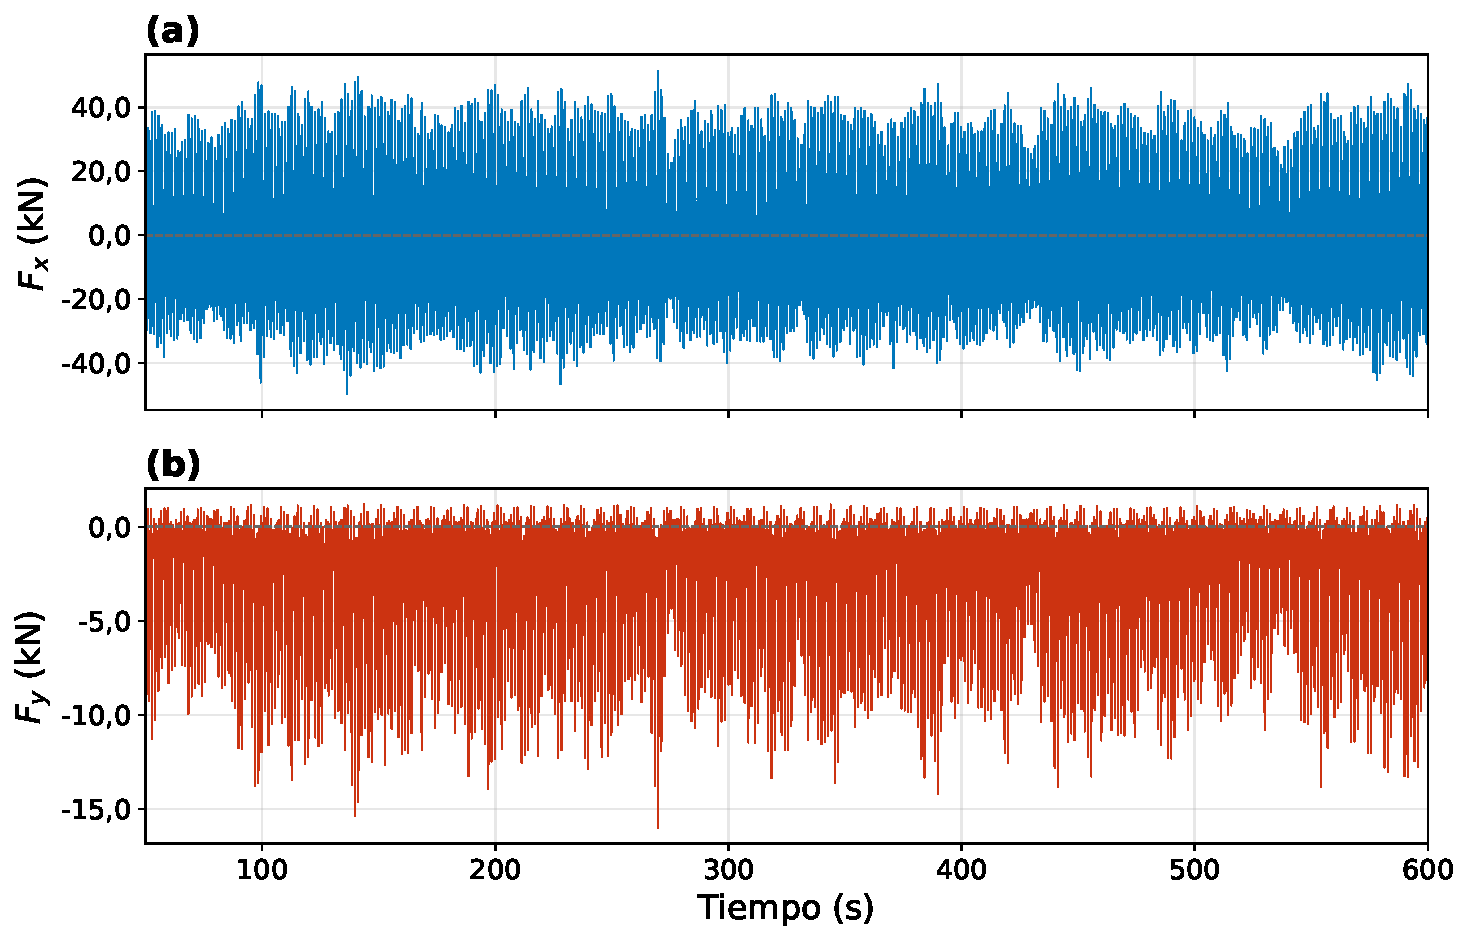
\includegraphics[width=0.85\textwidth]{Figuras/Figuras Anexo Fuerzas/fuerzas_xy_V14_S6.pdf}
    \caption{Fuerzas resultantes (a) $F_x$ y (b) $F_y$ en función del tiempo, $V = 14$~m/s, semilla $6$.}
    \label{fig:anexo_fuerzas_xy_V14_S6}
\end{figure}

\begin{figure}[H]
    \centering
    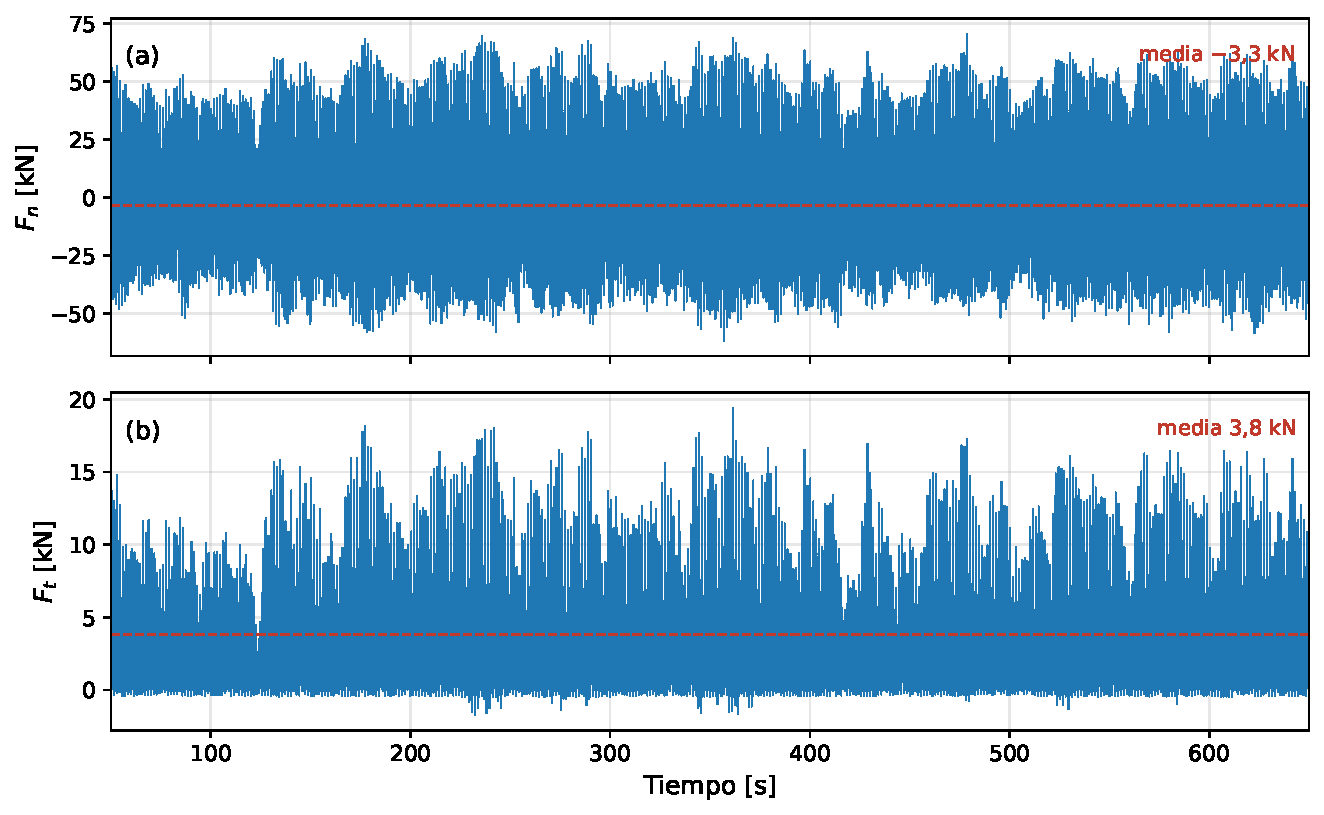
\includegraphics[width=0.85\textwidth]{Figuras/Figuras Anexo Fuerzas/fuerzas_xy_V16_S1.pdf}
    \caption{Fuerzas resultantes (a) $F_x$ y (b) $F_y$ en función del tiempo, $V = 16$~m/s, semilla $1$.}
    \label{fig:anexo_fuerzas_xy_V16_S1}
\end{figure}

\begin{figure}[H]
    \centering
    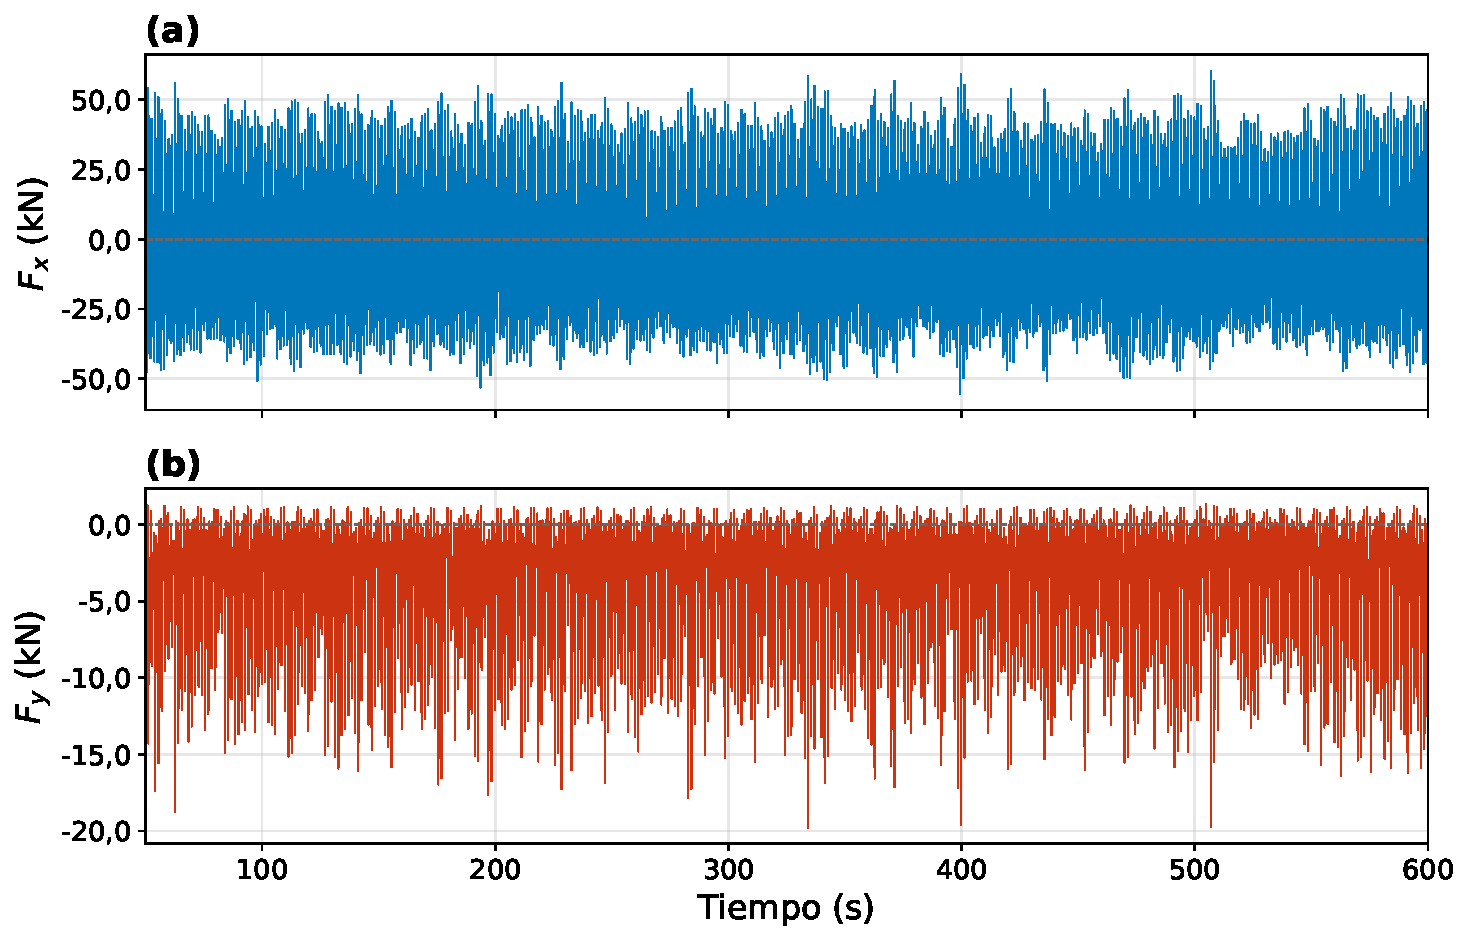
\includegraphics[width=0.85\textwidth]{Figuras/Figuras Anexo Fuerzas/fuerzas_xy_V16_S2.pdf}
    \caption{Fuerzas resultantes (a) $F_x$ y (b) $F_y$ en función del tiempo, $V = 16$~m/s, semilla $2$.}
    \label{fig:anexo_fuerzas_xy_V16_S2}
\end{figure}

\begin{figure}[H]
    \centering
    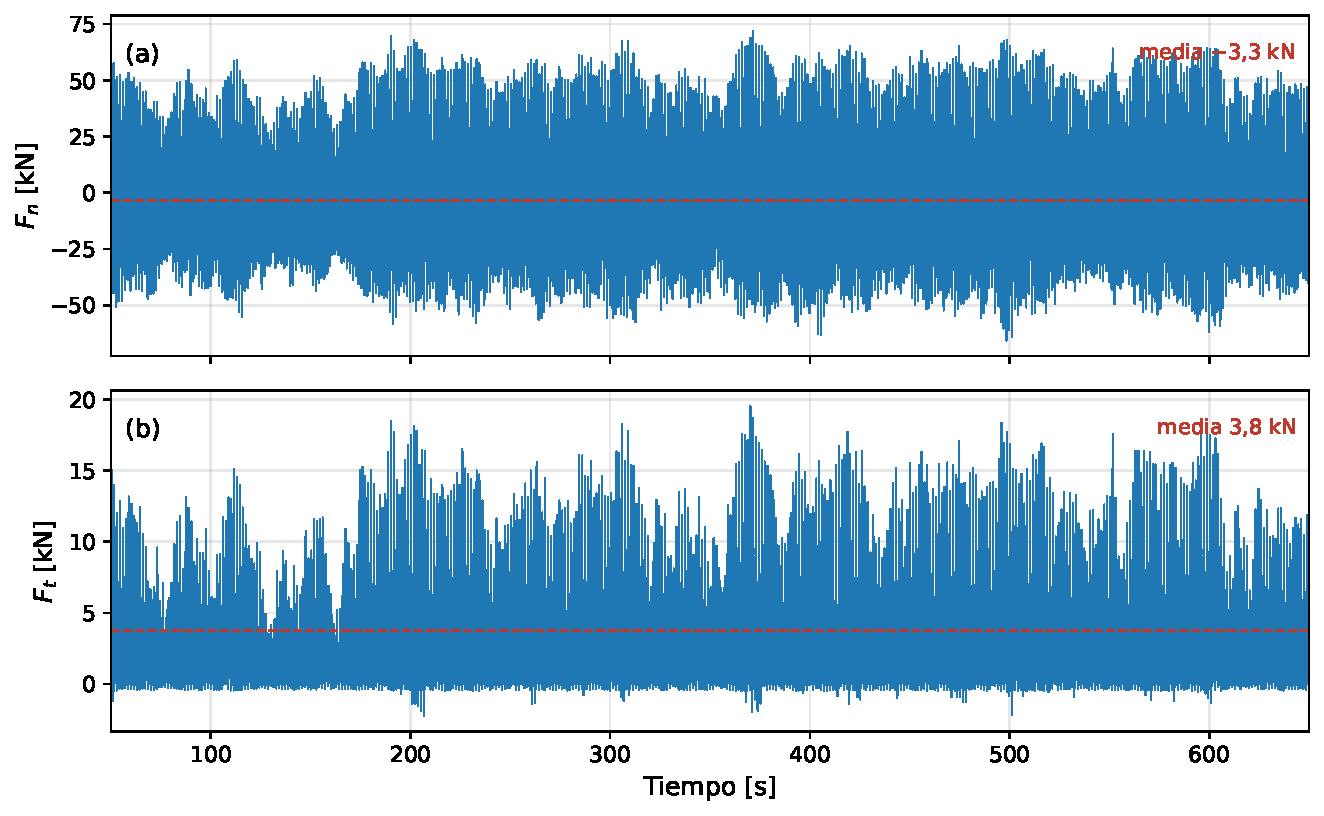
\includegraphics[width=0.85\textwidth]{Figuras/Figuras Anexo Fuerzas/fuerzas_xy_V16_S3.pdf}
    \caption{Fuerzas resultantes (a) $F_x$ y (b) $F_y$ en función del tiempo, $V = 16$~m/s, semilla $3$.}
    \label{fig:anexo_fuerzas_xy_V16_S3}
\end{figure}

\begin{figure}[H]
    \centering
    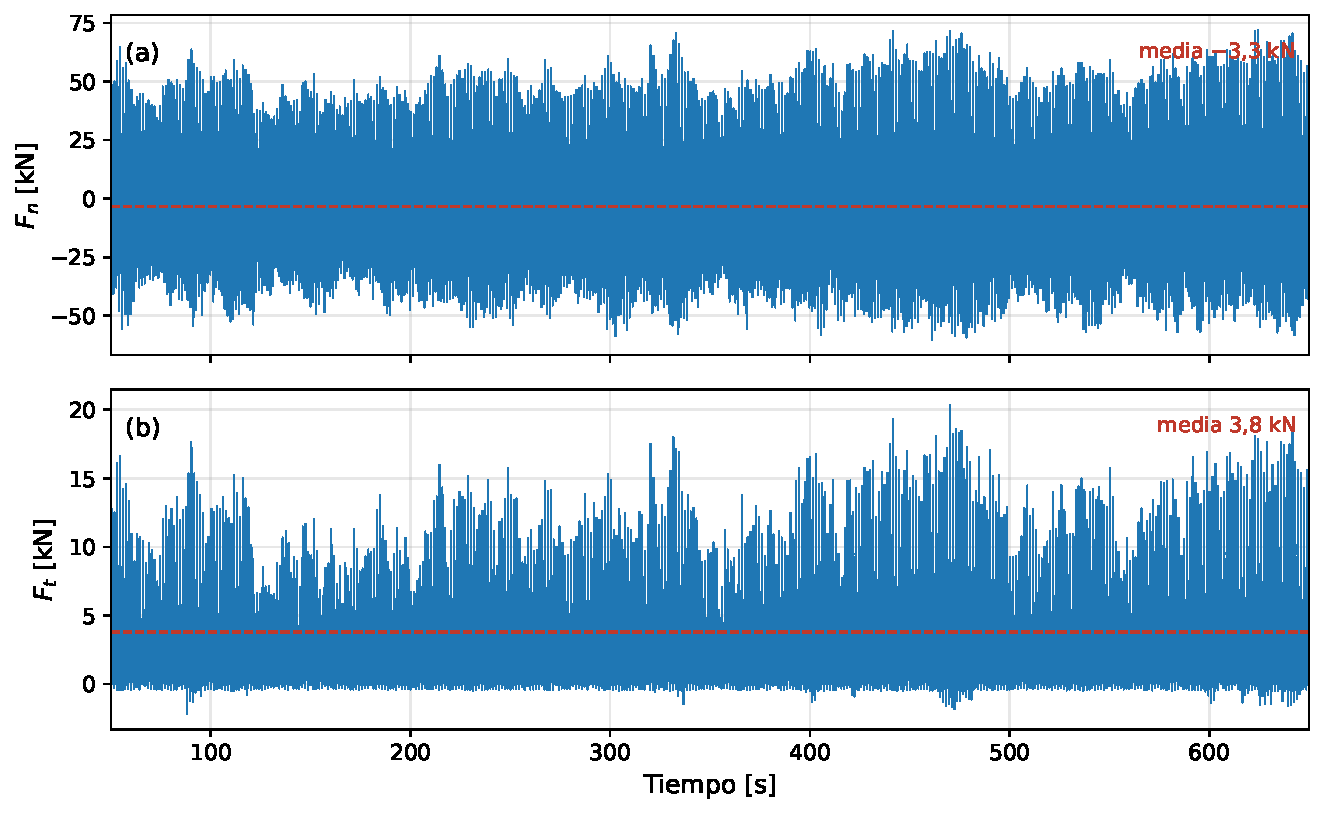
\includegraphics[width=0.85\textwidth]{Figuras/Figuras Anexo Fuerzas/fuerzas_xy_V16_S4.pdf}
    \caption{Fuerzas resultantes (a) $F_x$ y (b) $F_y$ en función del tiempo, $V = 16$~m/s, semilla $4$.}
    \label{fig:anexo_fuerzas_xy_V16_S4}
\end{figure}

\begin{figure}[H]
    \centering
    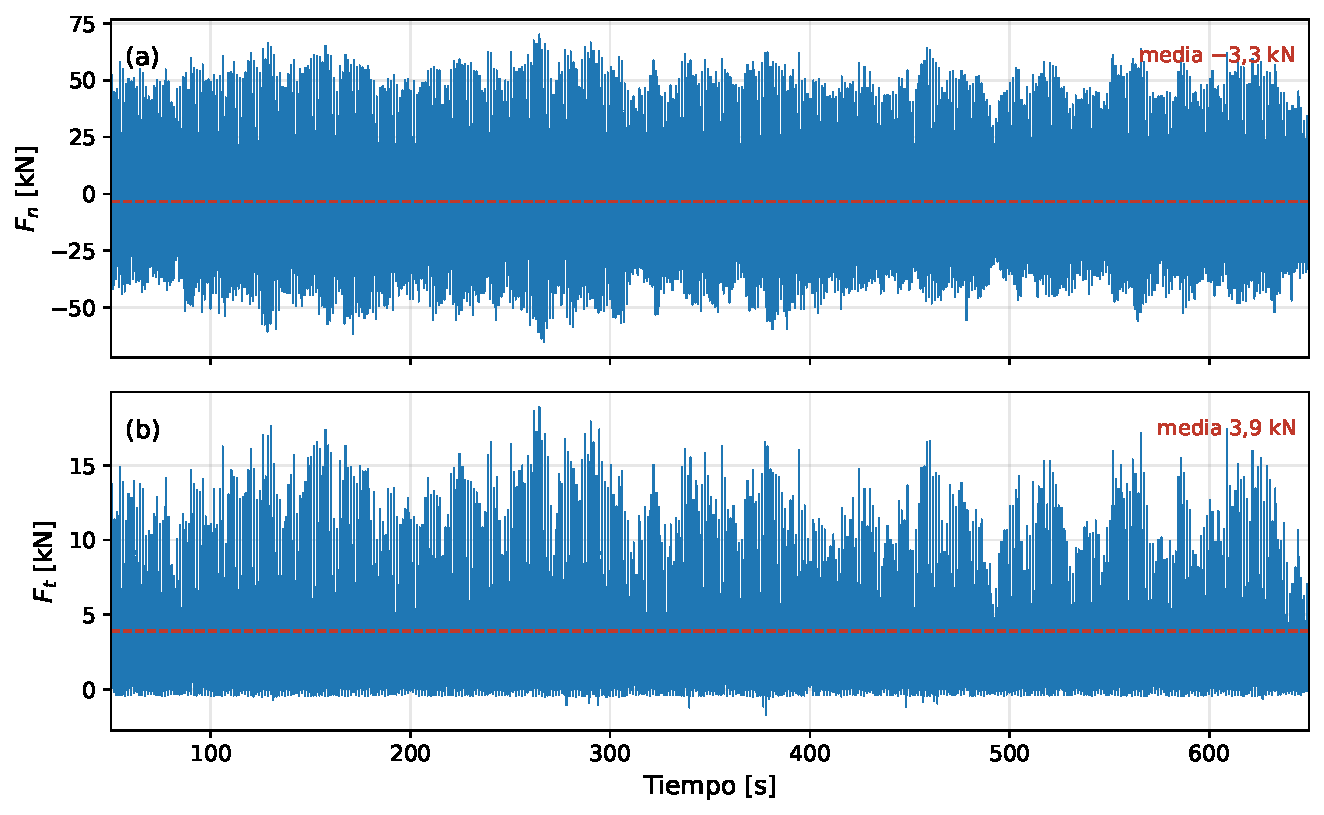
\includegraphics[width=0.85\textwidth]{Figuras/Figuras Anexo Fuerzas/fuerzas_xy_V16_S5.pdf}
    \caption{Fuerzas resultantes (a) $F_x$ y (b) $F_y$ en función del tiempo, $V = 16$~m/s, semilla $5$.}
    \label{fig:anexo_fuerzas_xy_V16_S5}
\end{figure}

\begin{figure}[H]
    \centering
    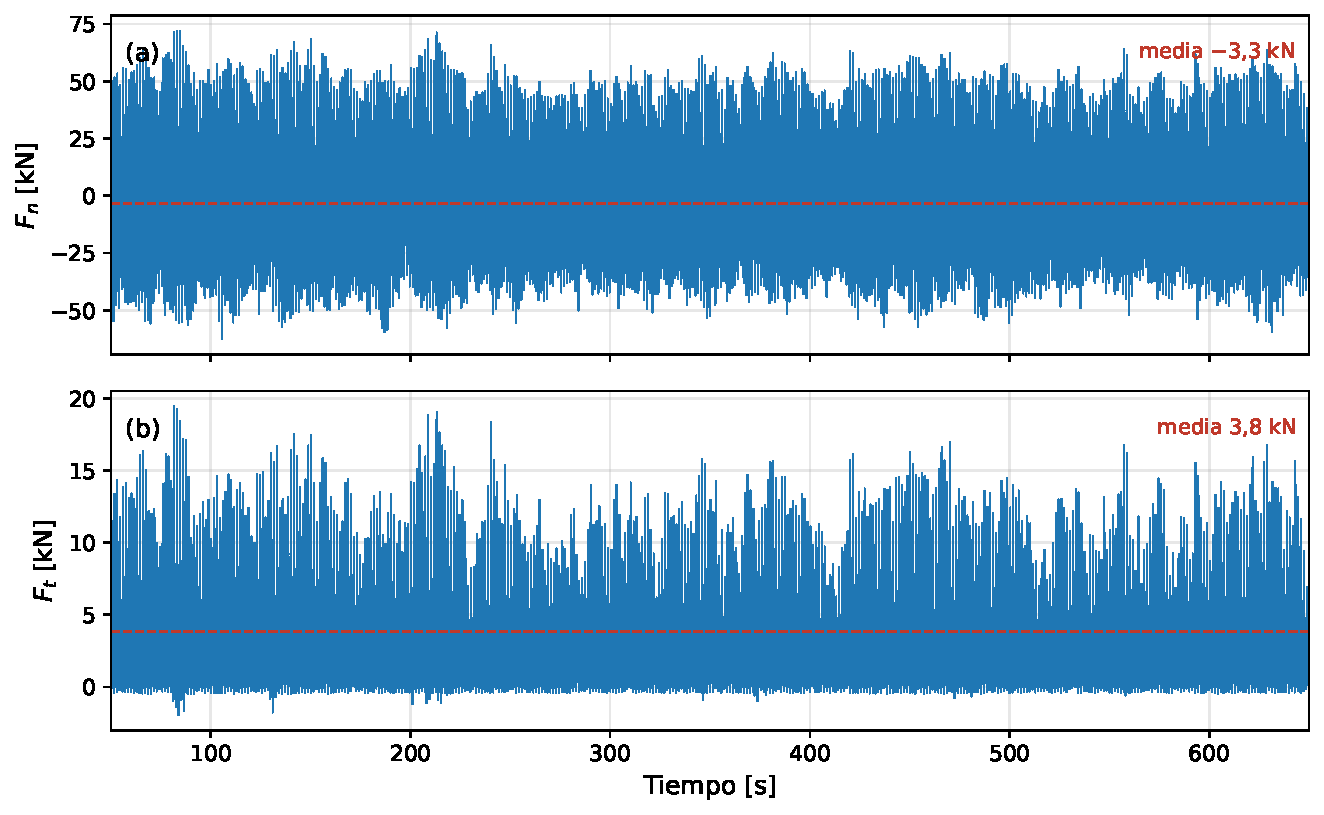
\includegraphics[width=0.85\textwidth]{Figuras/Figuras Anexo Fuerzas/fuerzas_xy_V16_S6.pdf}
    \caption{Fuerzas resultantes (a) $F_x$ y (b) $F_y$ en función del tiempo, $V = 16$~m/s, semilla $6$.}
    \label{fig:anexo_fuerzas_xy_V16_S6}
\end{figure}

\begin{figure}[H]
    \centering
    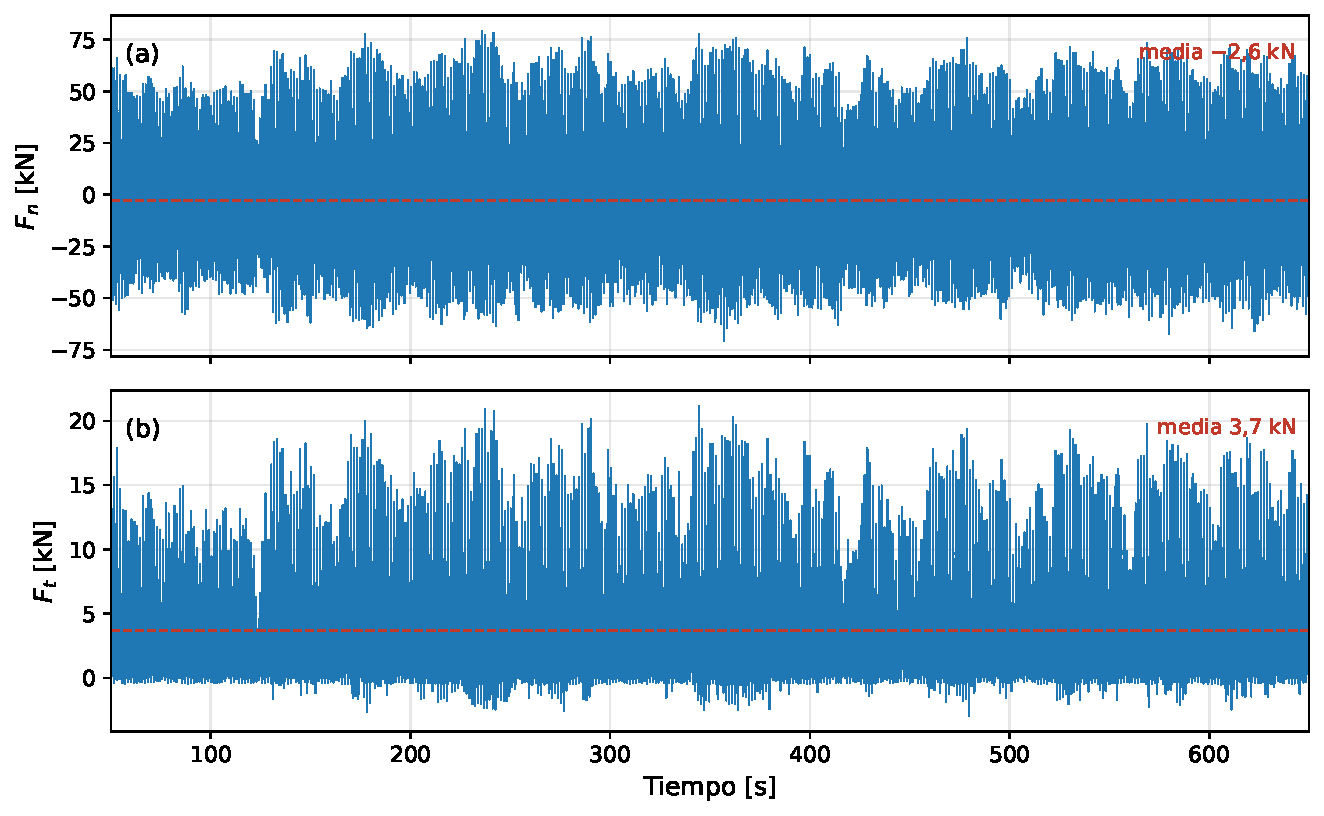
\includegraphics[width=0.85\textwidth]{Figuras/Figuras Anexo Fuerzas/fuerzas_xy_V18_S1.pdf}
    \caption{Fuerzas resultantes (a) $F_x$ y (b) $F_y$ en función del tiempo, $V = 18$~m/s, semilla $1$.}
    \label{fig:anexo_fuerzas_xy_V18_S1}
\end{figure}

\begin{figure}[H]
    \centering
    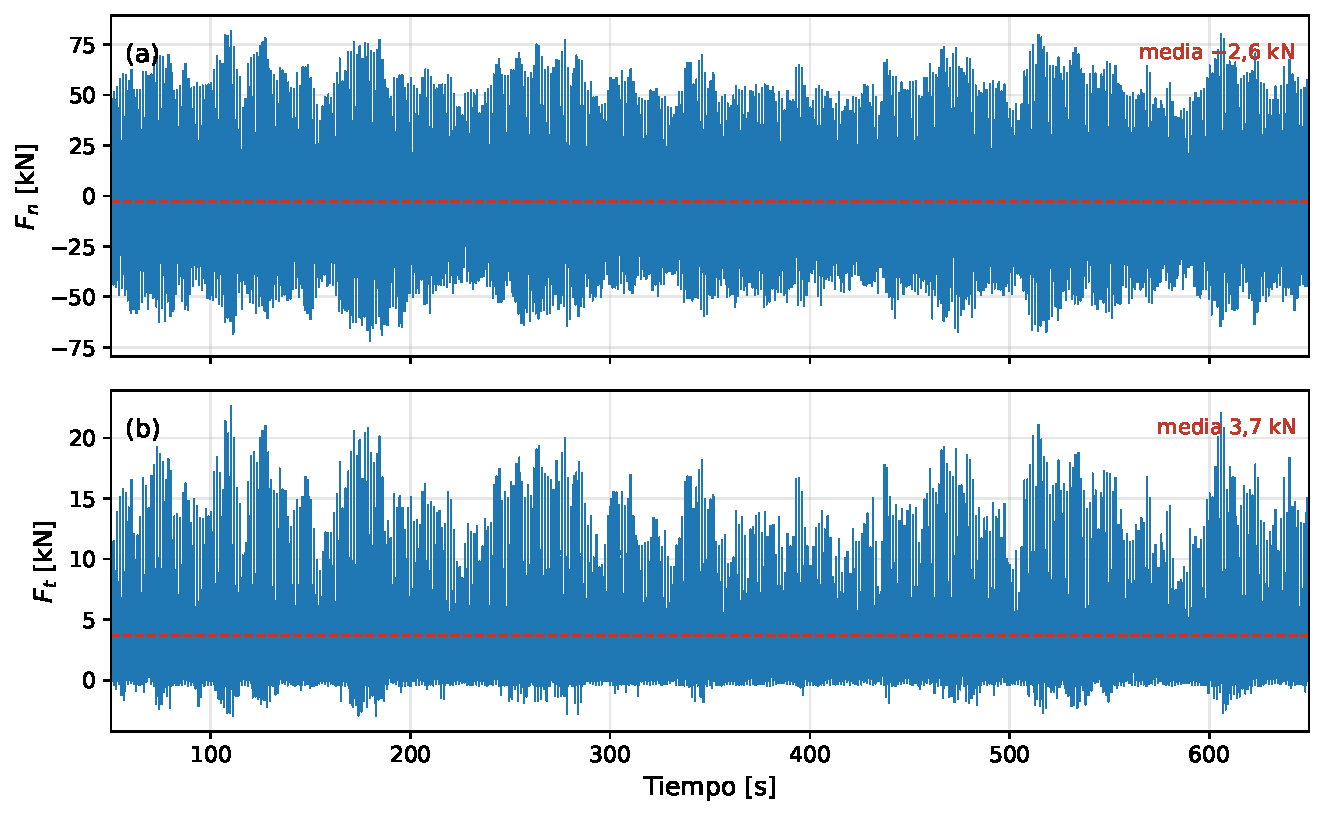
\includegraphics[width=0.85\textwidth]{Figuras/Figuras Anexo Fuerzas/fuerzas_xy_V18_S2.pdf}
    \caption{Fuerzas resultantes (a) $F_x$ y (b) $F_y$ en función del tiempo, $V = 18$~m/s, semilla $2$.}
    \label{fig:anexo_fuerzas_xy_V18_S2}
\end{figure}

\begin{figure}[H]
    \centering
    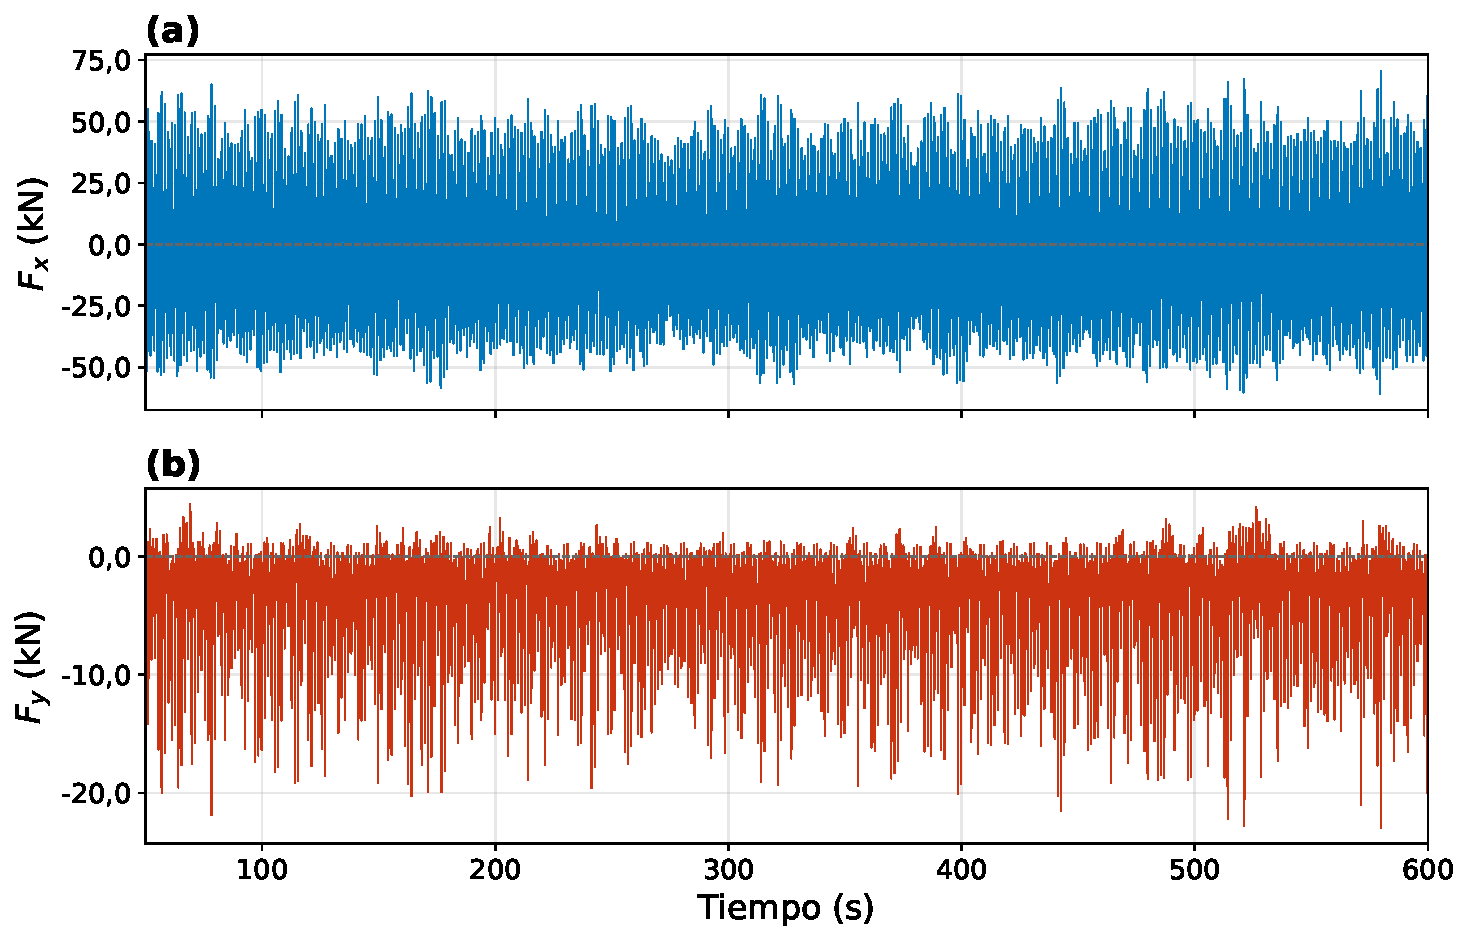
\includegraphics[width=0.85\textwidth]{Figuras/Figuras Anexo Fuerzas/fuerzas_xy_V18_S3.pdf}
    \caption{Fuerzas resultantes (a) $F_x$ y (b) $F_y$ en función del tiempo, $V = 18$~m/s, semilla $3$.}
    \label{fig:anexo_fuerzas_xy_V18_S3}
\end{figure}

\begin{figure}[H]
    \centering
    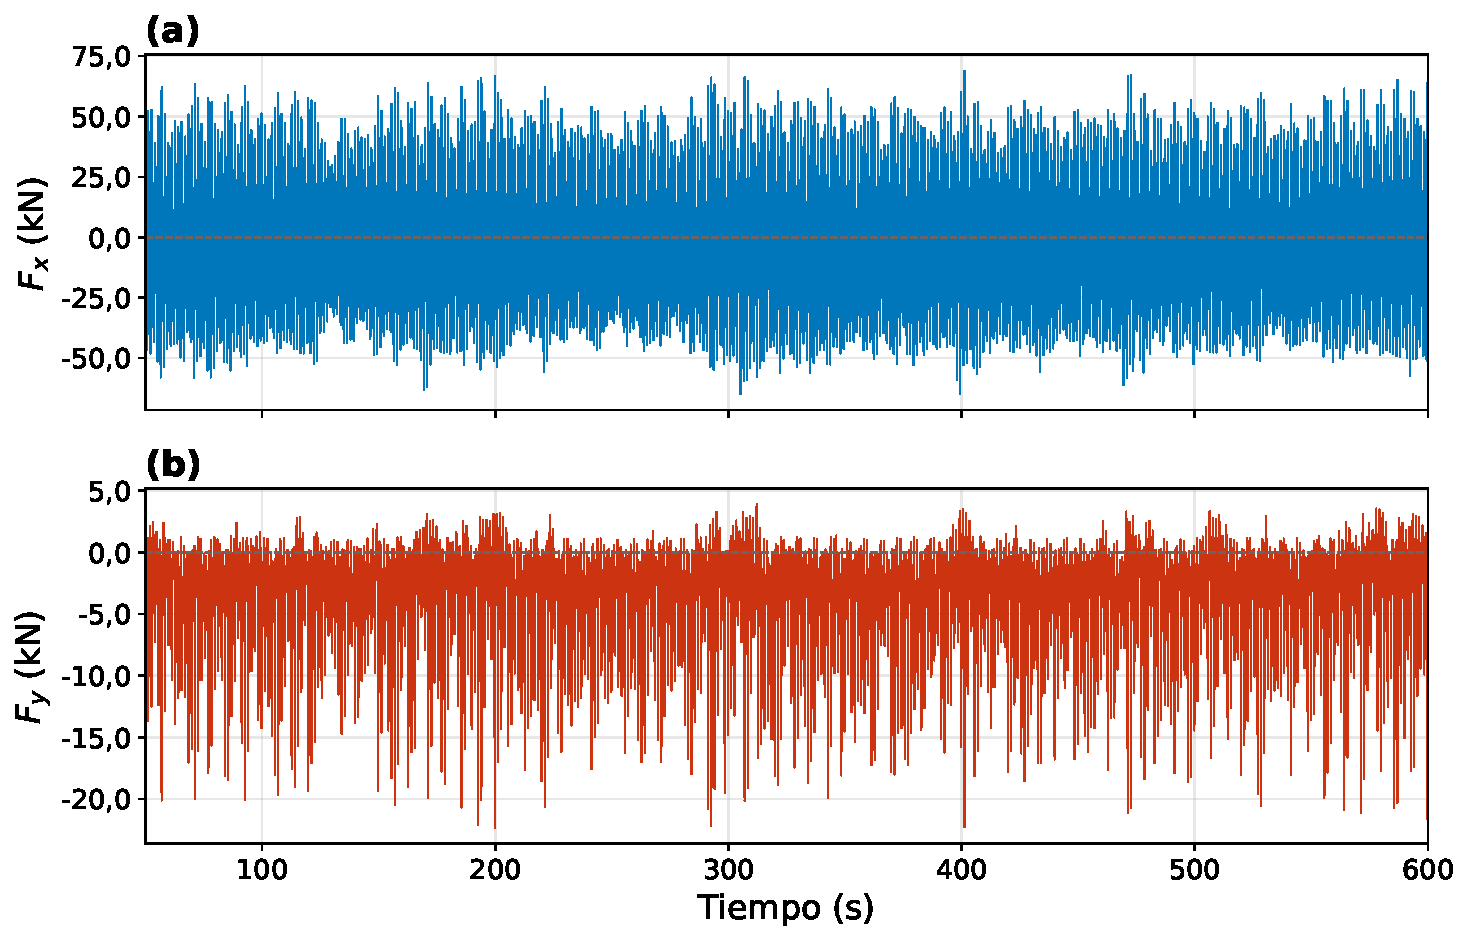
\includegraphics[width=0.85\textwidth]{Figuras/Figuras Anexo Fuerzas/fuerzas_xy_V18_S4.pdf}
    \caption{Fuerzas resultantes (a) $F_x$ y (b) $F_y$ en función del tiempo, $V = 18$~m/s, semilla $4$.}
    \label{fig:anexo_fuerzas_xy_V18_S4}
\end{figure}

\begin{figure}[H]
    \centering
    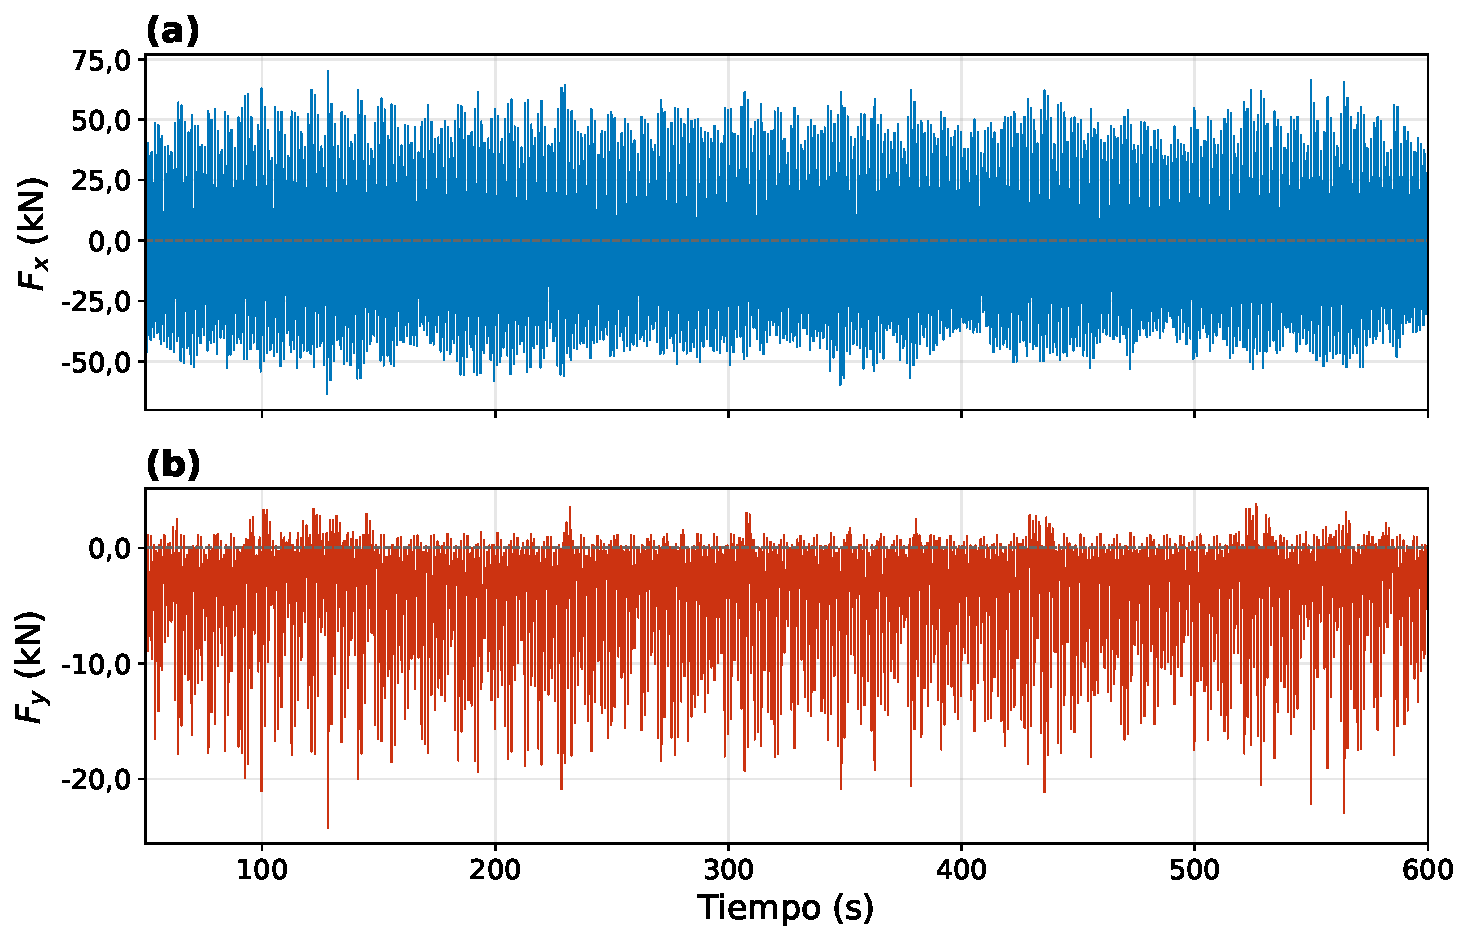
\includegraphics[width=0.85\textwidth]{Figuras/Figuras Anexo Fuerzas/fuerzas_xy_V18_S5.pdf}
    \caption{Fuerzas resultantes (a) $F_x$ y (b) $F_y$ en función del tiempo, $V = 18$~m/s, semilla $5$.}
    \label{fig:anexo_fuerzas_xy_V18_S5}
\end{figure}

\begin{figure}[H]
    \centering
    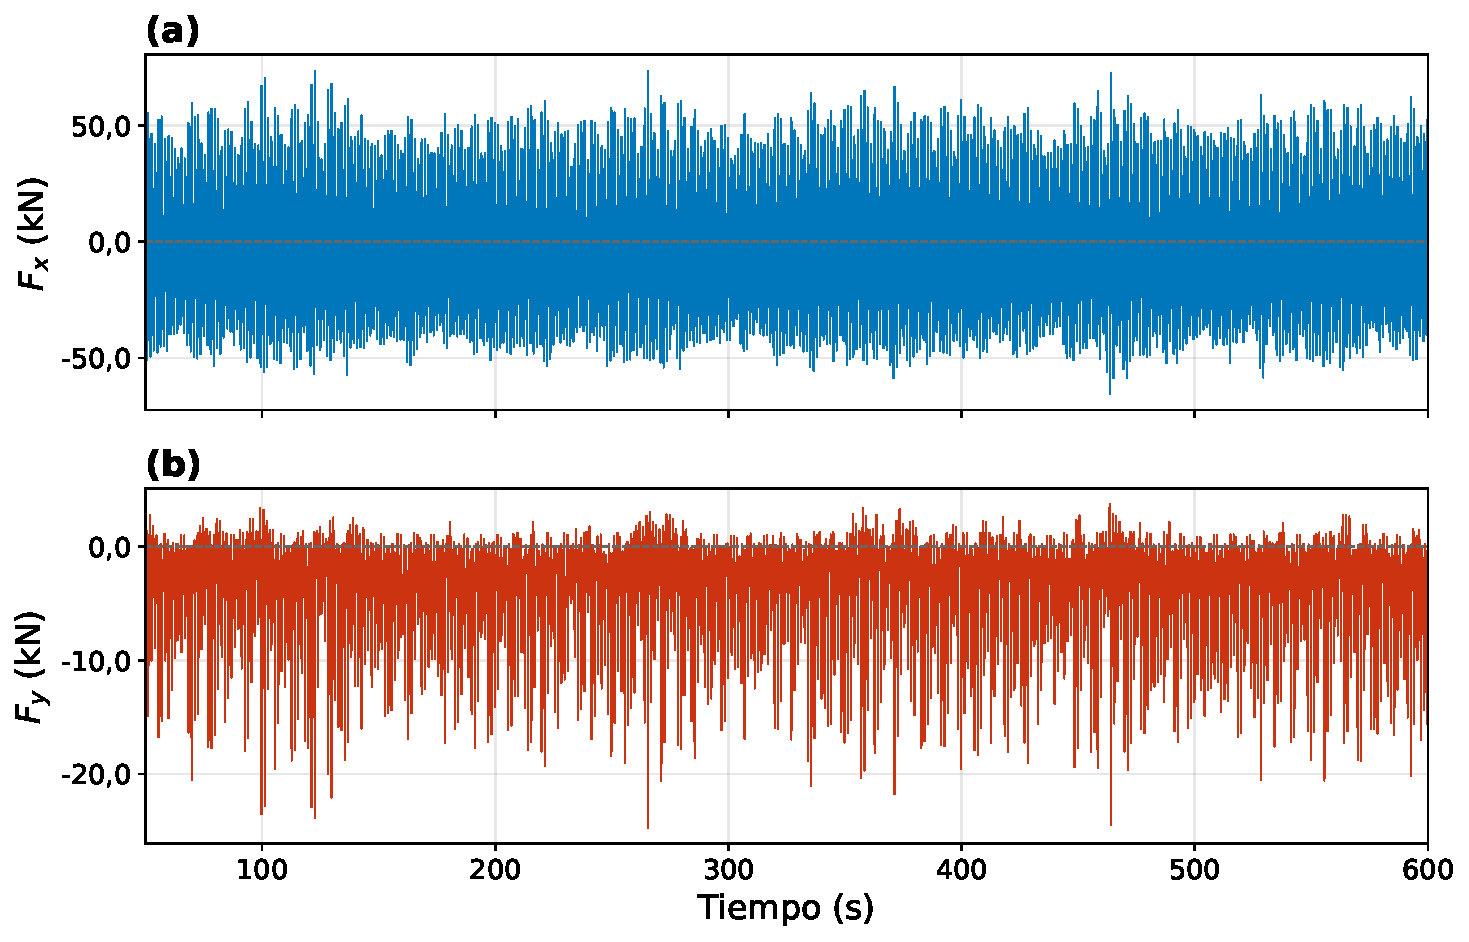
\includegraphics[width=0.85\textwidth]{Figuras/Figuras Anexo Fuerzas/fuerzas_xy_V18_S6.pdf}
    \caption{Fuerzas resultantes (a) $F_x$ y (b) $F_y$ en función del tiempo, $V = 18$~m/s, semilla $6$.}
    \label{fig:anexo_fuerzas_xy_V18_S6}
\end{figure}

\begin{figure}[H]
    \centering
    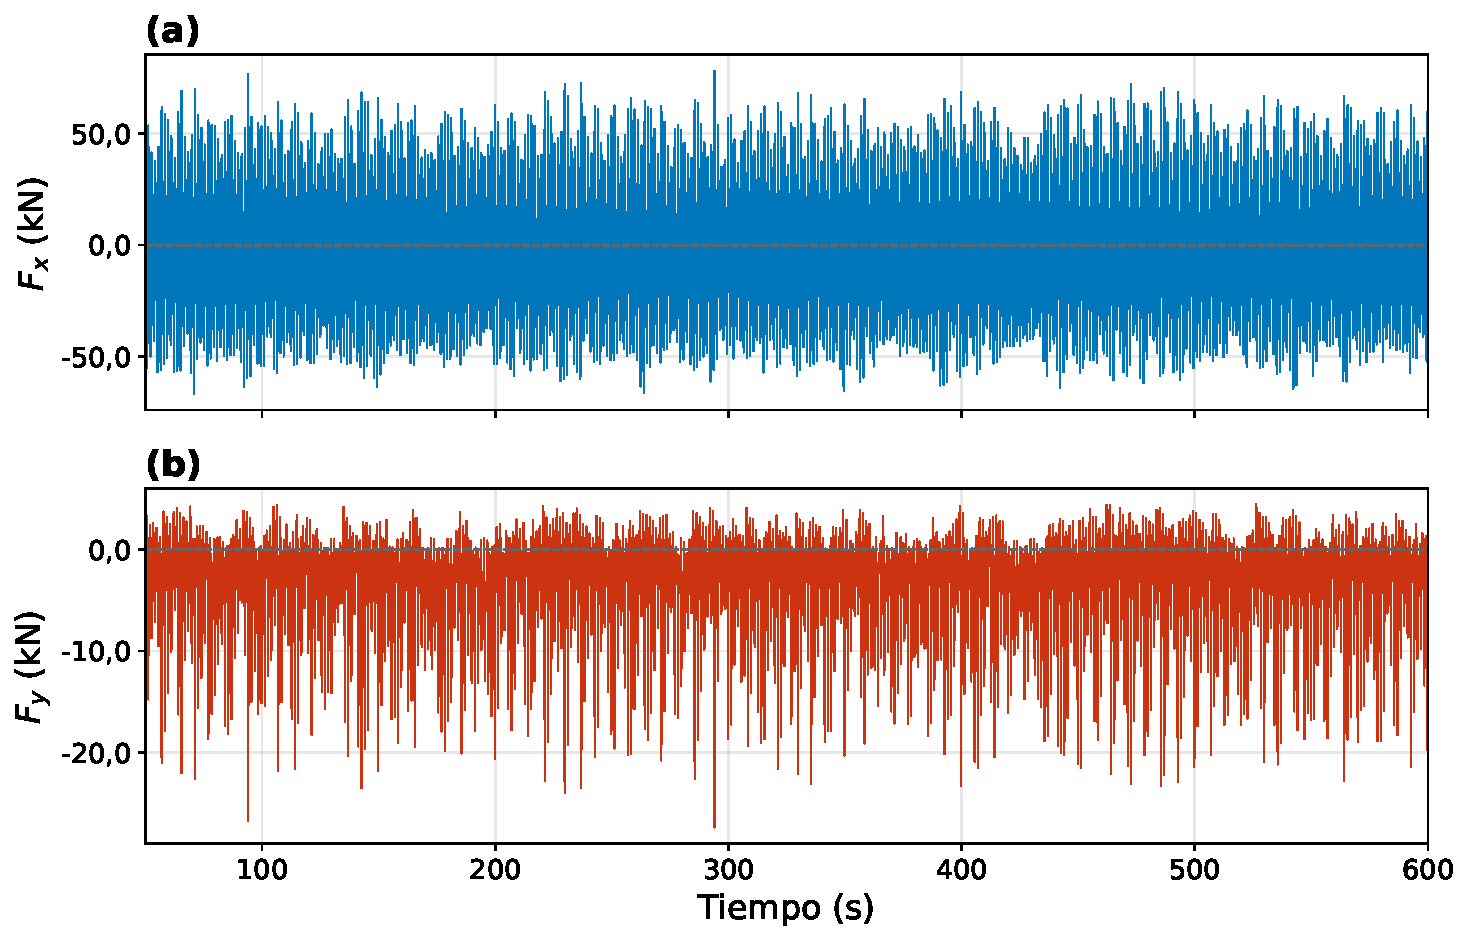
\includegraphics[width=0.85\textwidth]{Figuras/Figuras Anexo Fuerzas/fuerzas_xy_V20_S1.pdf}
    \caption{Fuerzas resultantes (a) $F_x$ y (b) $F_y$ en función del tiempo, $V = 20$~m/s, semilla $1$.}
    \label{fig:anexo_fuerzas_xy_V20_S1}
\end{figure}

\begin{figure}[H]
    \centering
    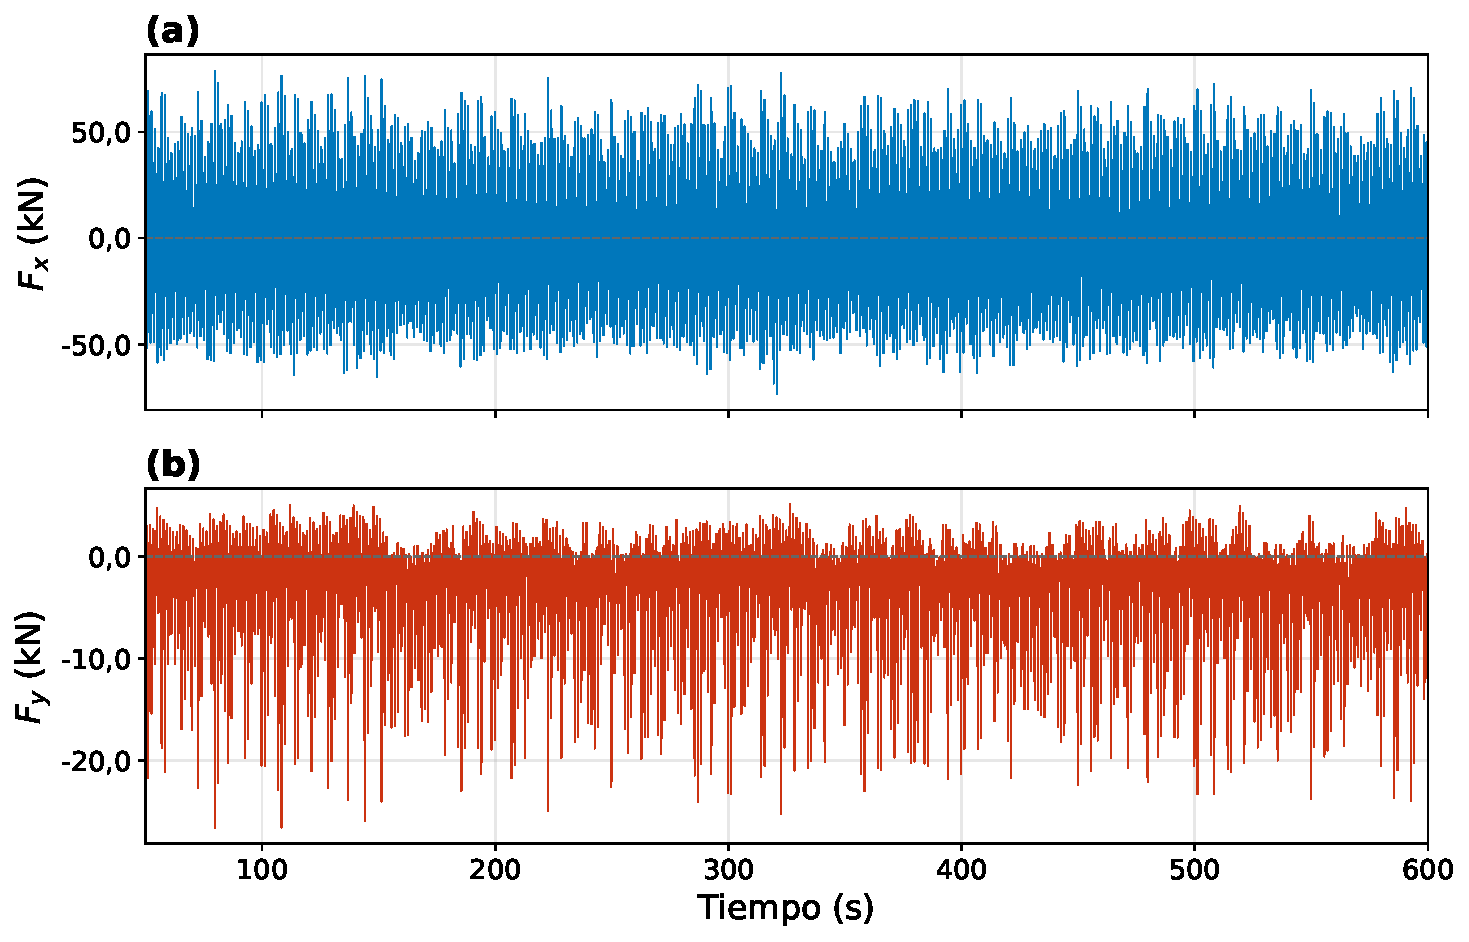
\includegraphics[width=0.85\textwidth]{Figuras/Figuras Anexo Fuerzas/fuerzas_xy_V20_S2.pdf}
    \caption{Fuerzas resultantes (a) $F_x$ y (b) $F_y$ en función del tiempo, $V = 20$~m/s, semilla $2$.}
    \label{fig:anexo_fuerzas_xy_V20_S2}
\end{figure}

\begin{figure}[H]
    \centering
    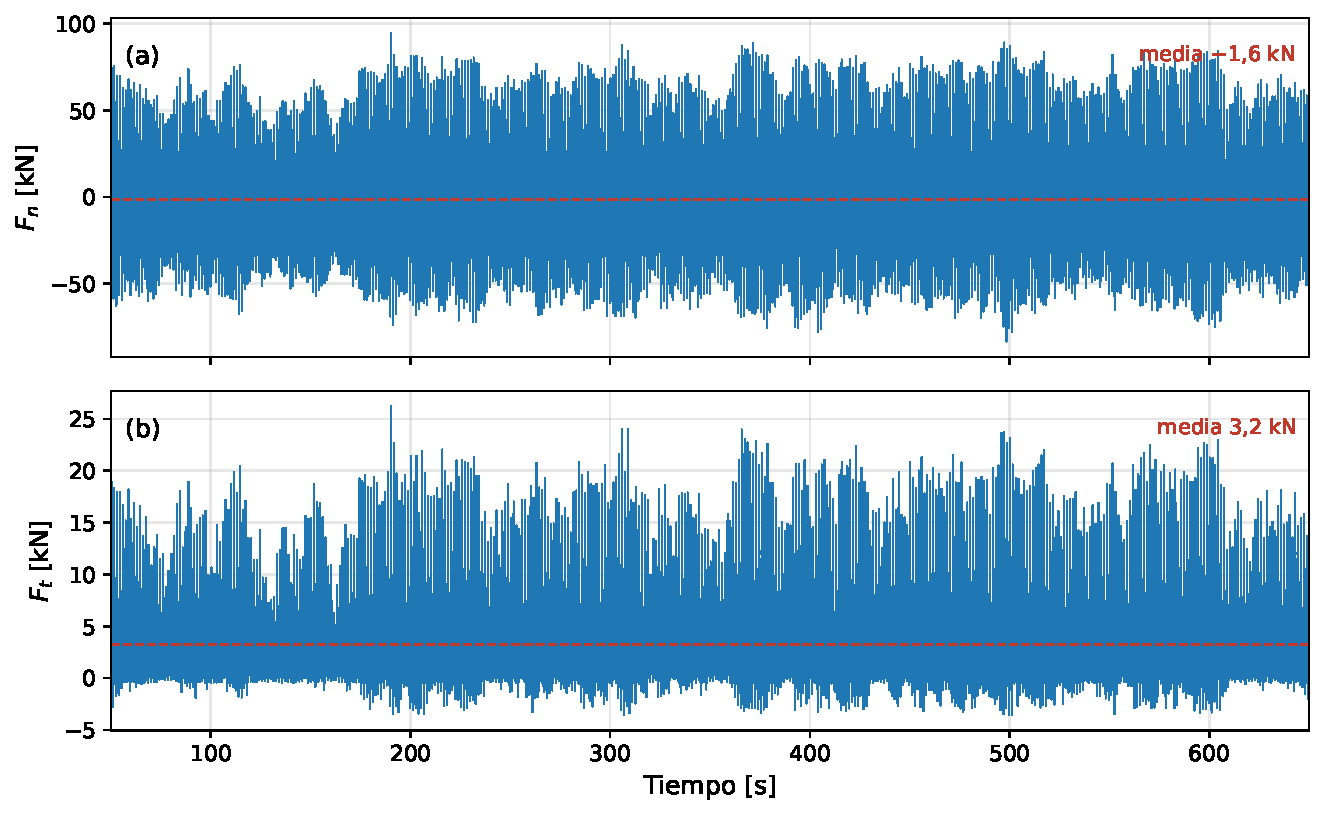
\includegraphics[width=0.85\textwidth]{Figuras/Figuras Anexo Fuerzas/fuerzas_xy_V20_S3.pdf}
    \caption{Fuerzas resultantes (a) $F_x$ y (b) $F_y$ en función del tiempo, $V = 20$~m/s, semilla $3$.}
    \label{fig:anexo_fuerzas_xy_V20_S3}
\end{figure}

\begin{figure}[H]
    \centering
    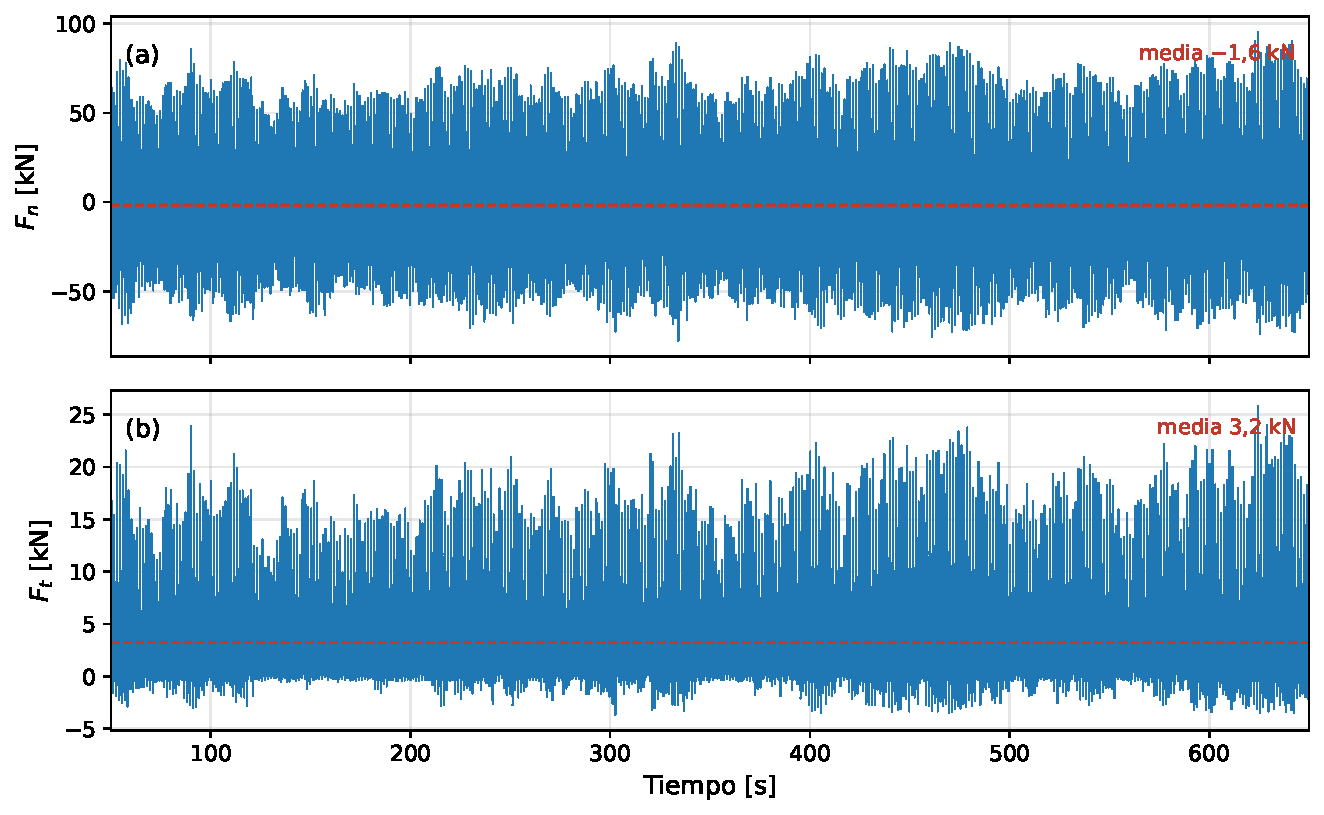
\includegraphics[width=0.85\textwidth]{Figuras/Figuras Anexo Fuerzas/fuerzas_xy_V20_S4.pdf}
    \caption{Fuerzas resultantes (a) $F_x$ y (b) $F_y$ en función del tiempo, $V = 20$~m/s, semilla $4$.}
    \label{fig:anexo_fuerzas_xy_V20_S4}
\end{figure}

\begin{figure}[H]
    \centering
    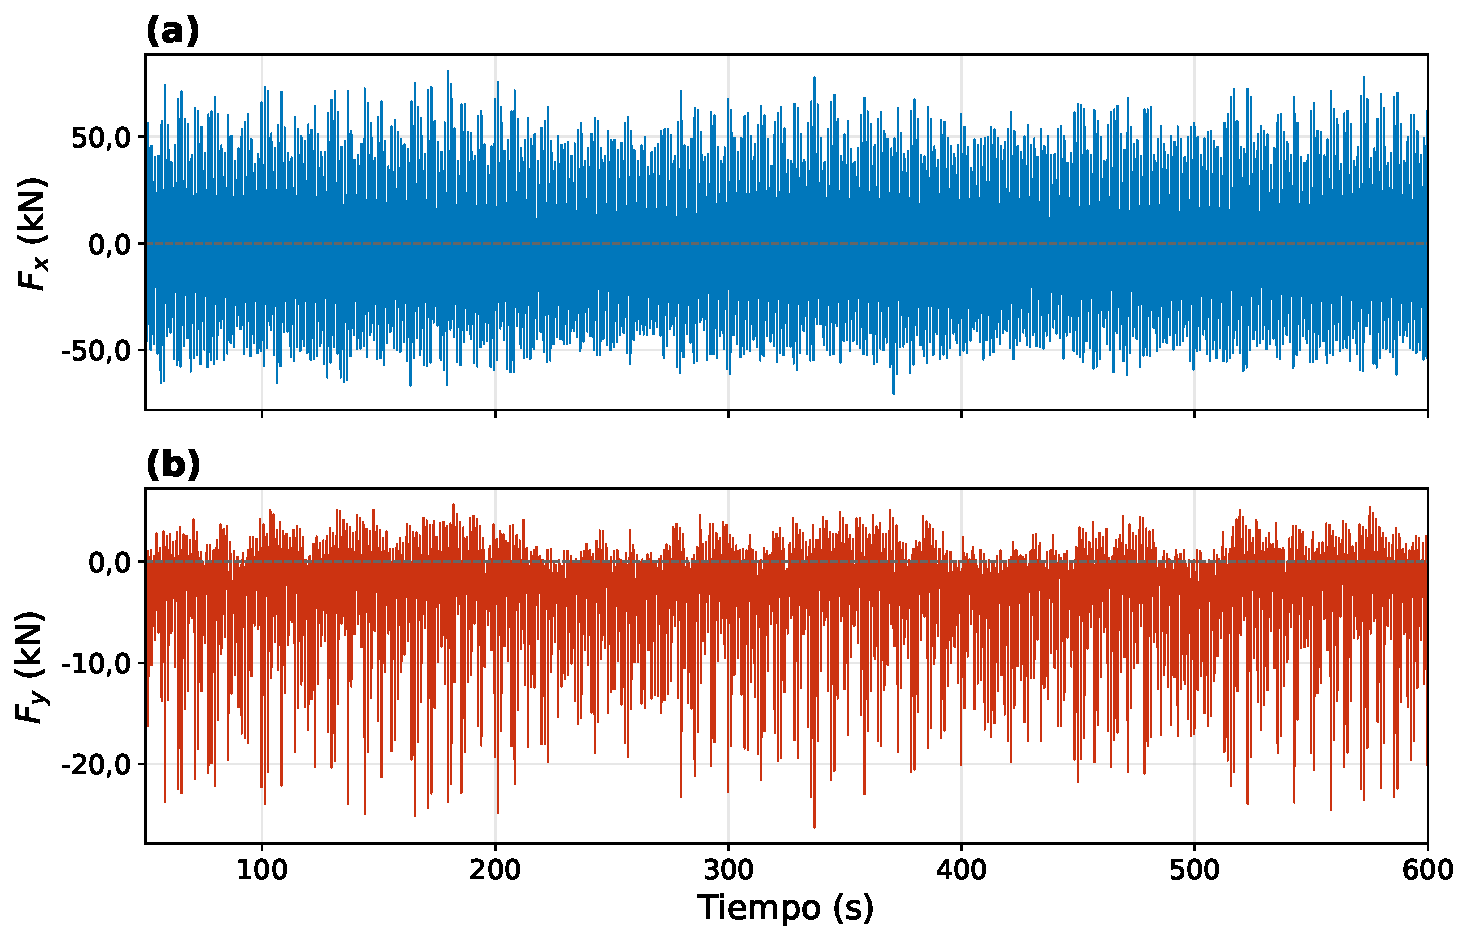
\includegraphics[width=0.85\textwidth]{Figuras/Figuras Anexo Fuerzas/fuerzas_xy_V20_S5.pdf}
    \caption{Fuerzas resultantes (a) $F_x$ y (b) $F_y$ en función del tiempo, $V = 20$~m/s, semilla $5$.}
    \label{fig:anexo_fuerzas_xy_V20_S5}
\end{figure}

\begin{figure}[H]
    \centering
    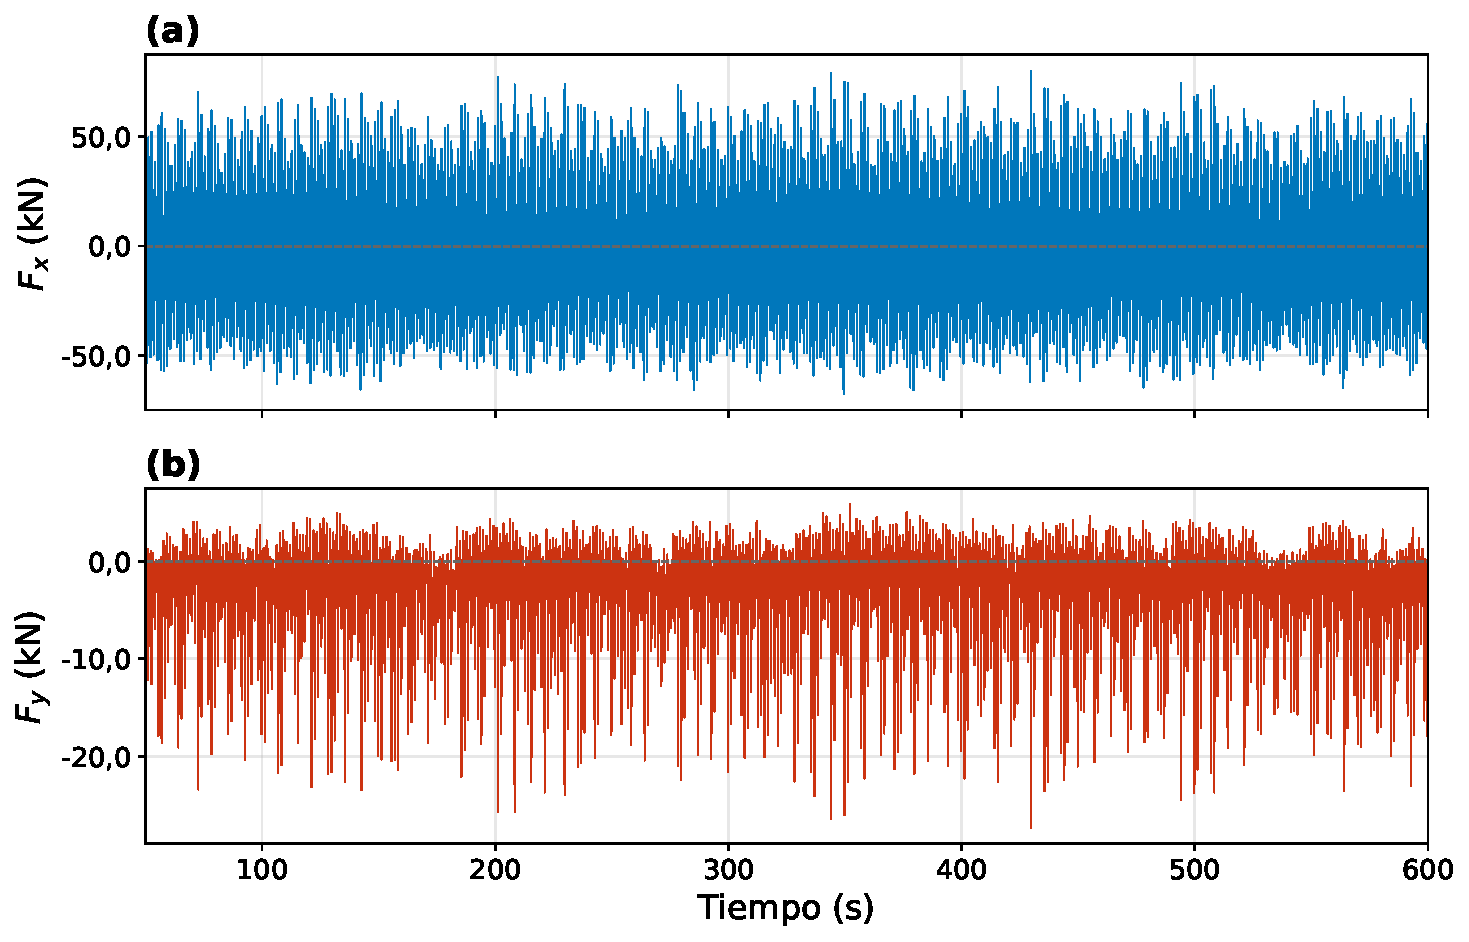
\includegraphics[width=0.85\textwidth]{Figuras/Figuras Anexo Fuerzas/fuerzas_xy_V20_S6.pdf}
    \caption{Fuerzas resultantes (a) $F_x$ y (b) $F_y$ en función del tiempo, $V = 20$~m/s, semilla $6$.}
    \label{fig:anexo_fuerzas_xy_V20_S6}
\end{figure}

\begin{figure}[H]
    \centering
    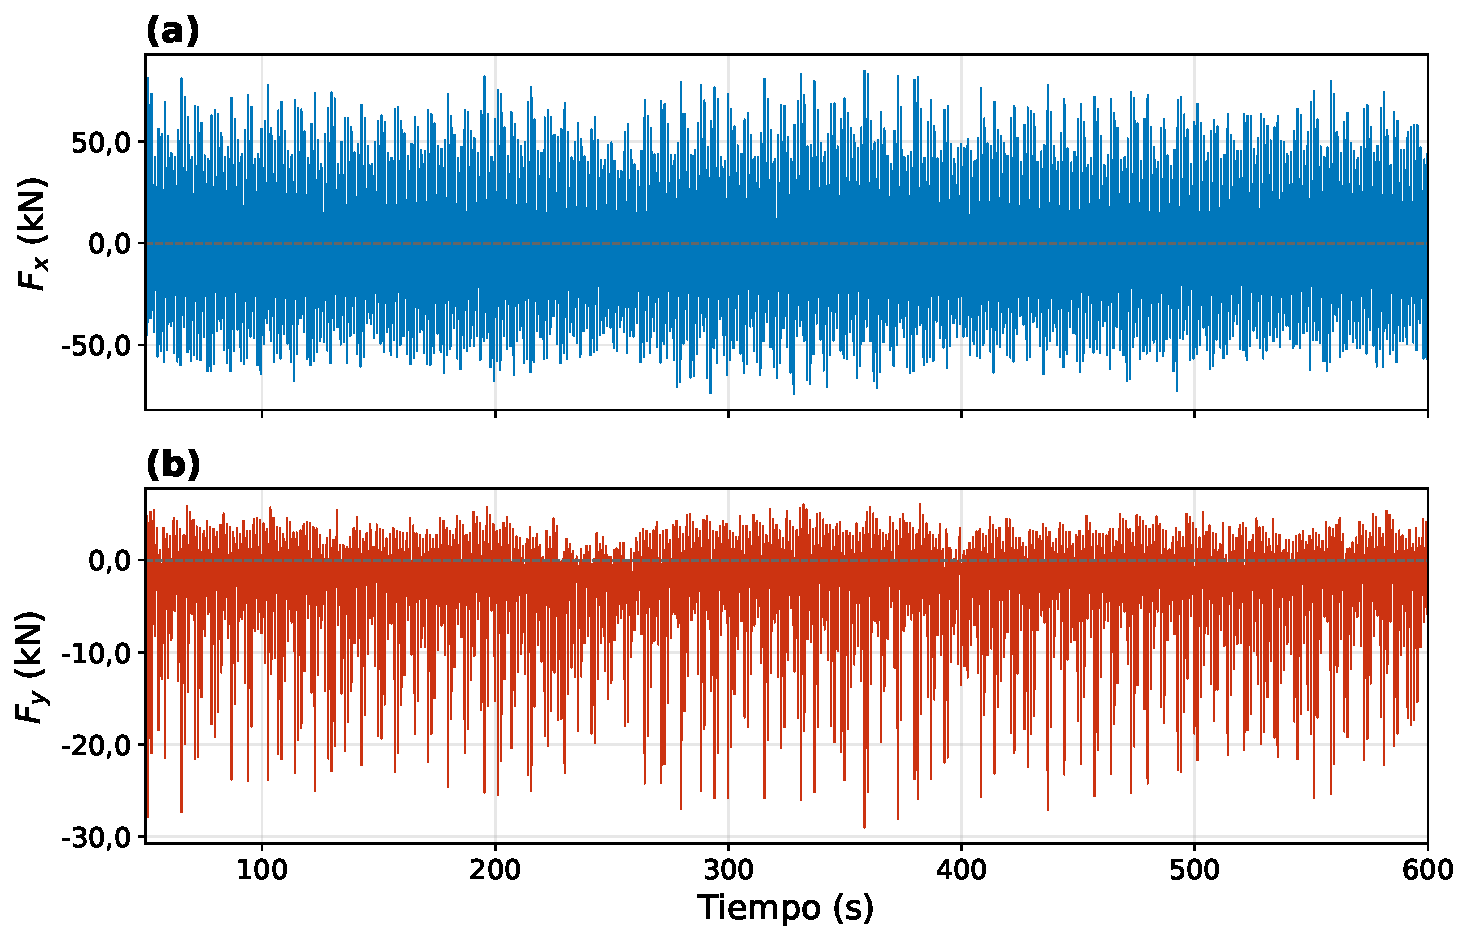
\includegraphics[width=0.85\textwidth]{Figuras/Figuras Anexo Fuerzas/fuerzas_xy_V22_S1.pdf}
    \caption{Fuerzas resultantes (a) $F_x$ y (b) $F_y$ en función del tiempo, $V = 22$~m/s, semilla $1$.}
    \label{fig:anexo_fuerzas_xy_V22_S1}
\end{figure}

\begin{figure}[H]
    \centering
    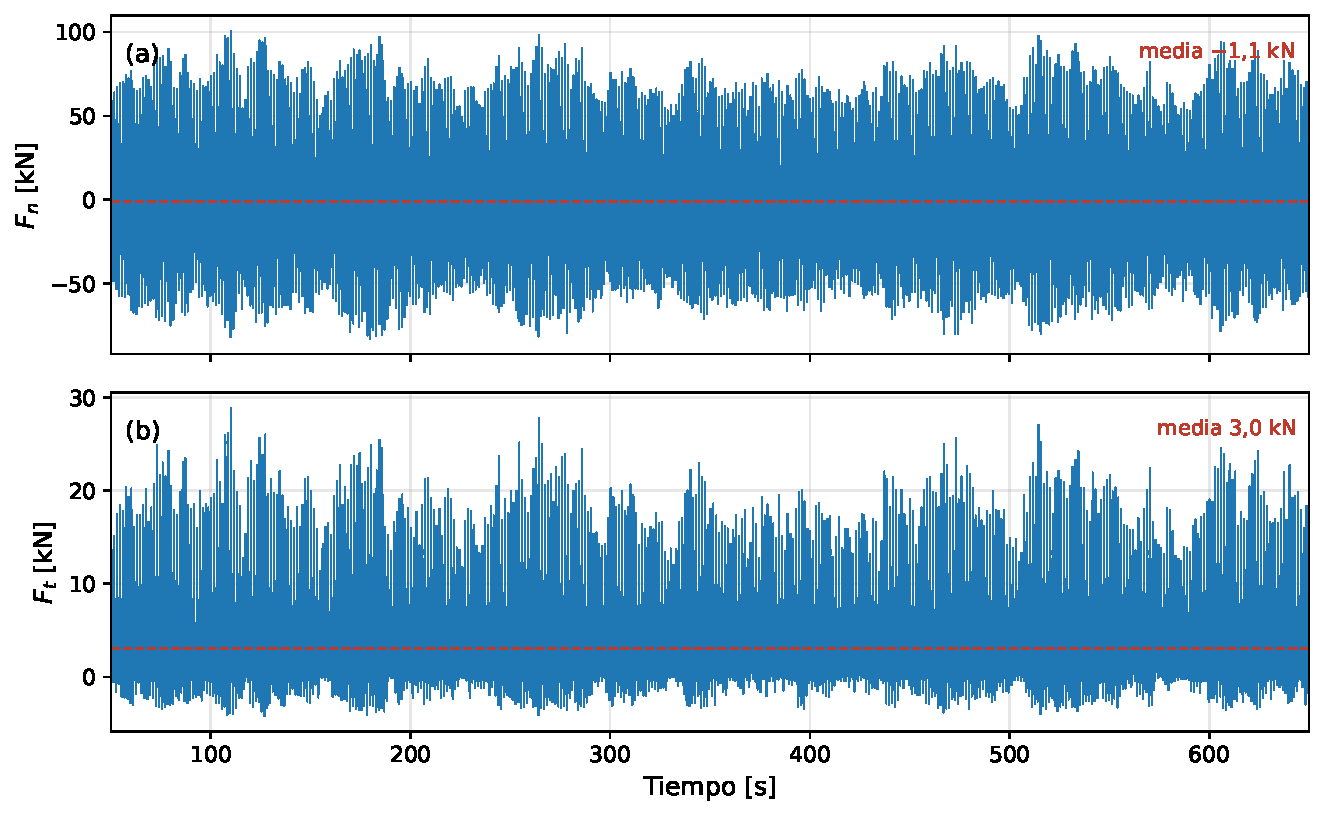
\includegraphics[width=0.85\textwidth]{Figuras/Figuras Anexo Fuerzas/fuerzas_xy_V22_S2.pdf}
    \caption{Fuerzas resultantes (a) $F_x$ y (b) $F_y$ en función del tiempo, $V = 22$~m/s, semilla $2$.}
    \label{fig:anexo_fuerzas_xy_V22_S2}
\end{figure}

\begin{figure}[H]
    \centering
    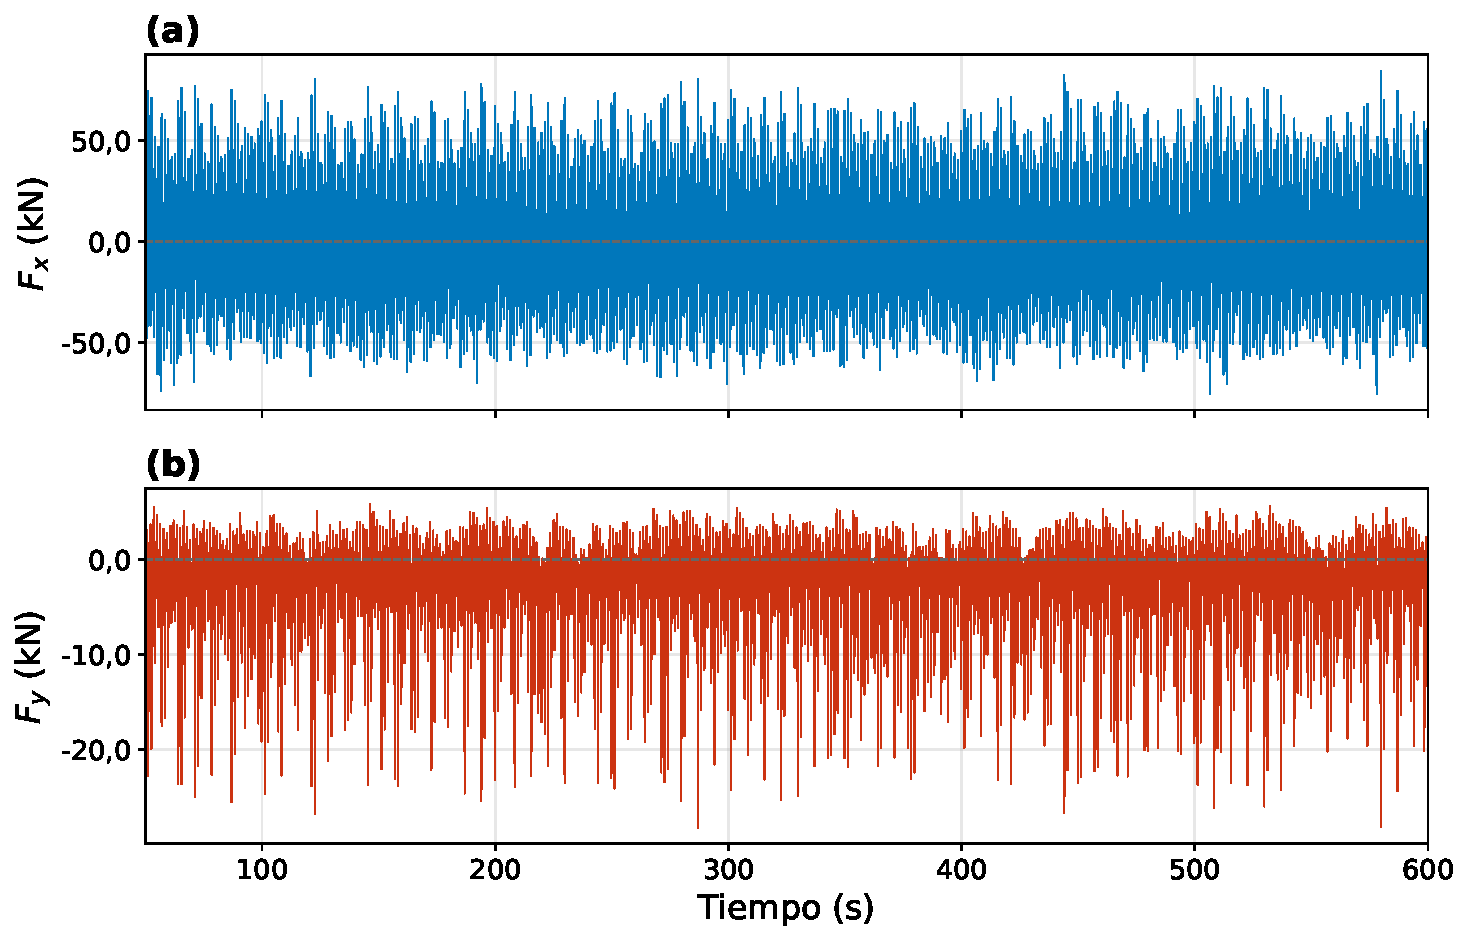
\includegraphics[width=0.85\textwidth]{Figuras/Figuras Anexo Fuerzas/fuerzas_xy_V22_S3.pdf}
    \caption{Fuerzas resultantes (a) $F_x$ y (b) $F_y$ en función del tiempo, $V = 22$~m/s, semilla $3$.}
    \label{fig:anexo_fuerzas_xy_V22_S3}
\end{figure}

\begin{figure}[H]
    \centering
    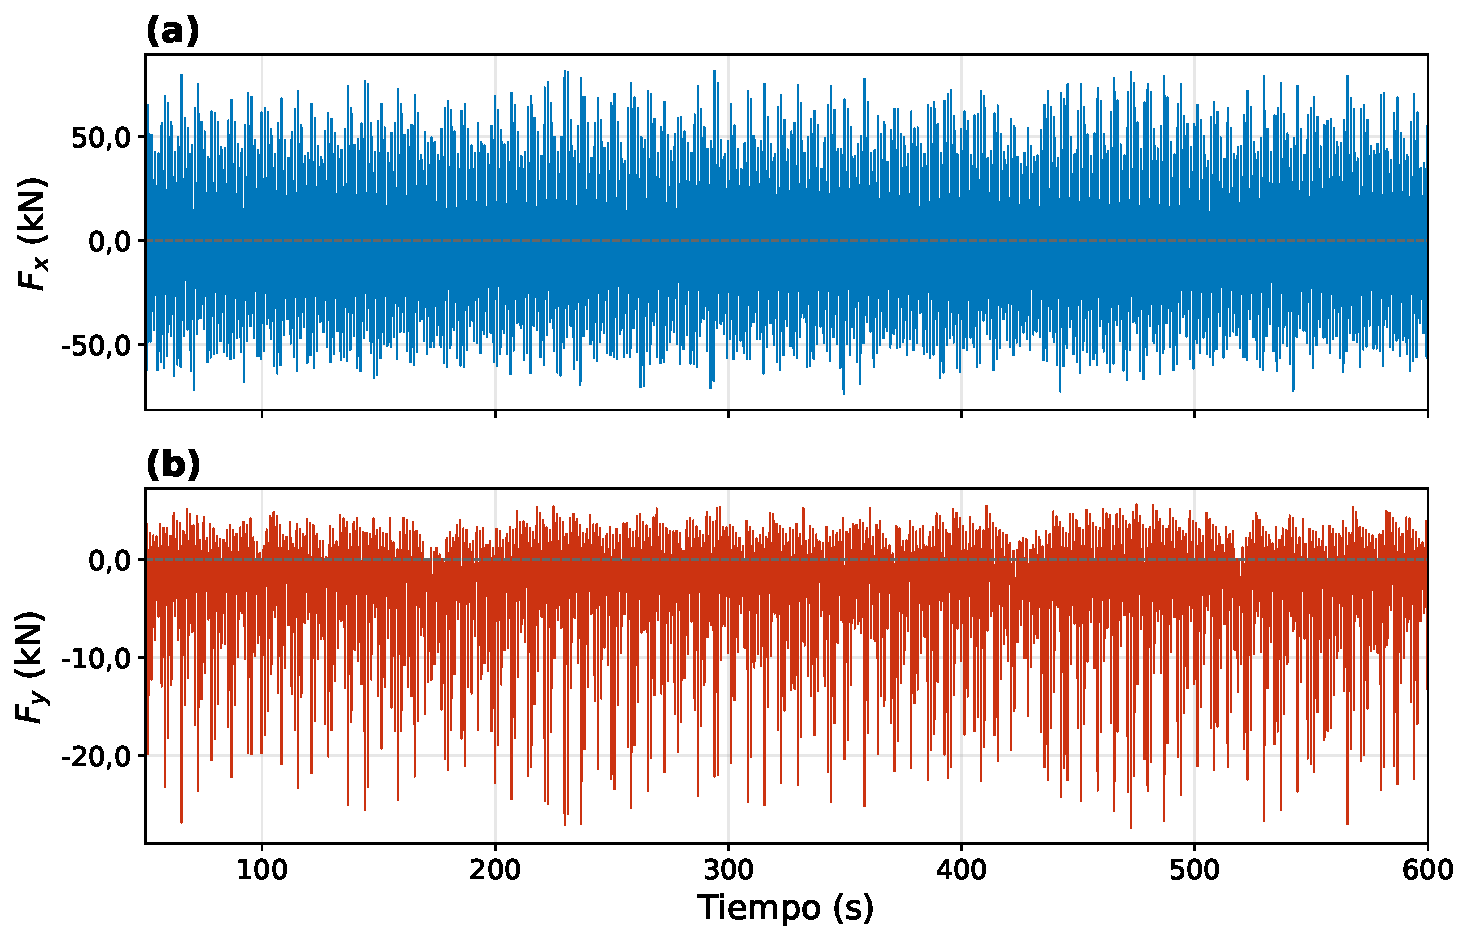
\includegraphics[width=0.85\textwidth]{Figuras/Figuras Anexo Fuerzas/fuerzas_xy_V22_S4.pdf}
    \caption{Fuerzas resultantes (a) $F_x$ y (b) $F_y$ en función del tiempo, $V = 22$~m/s, semilla $4$.}
    \label{fig:anexo_fuerzas_xy_V22_S4}
\end{figure}

\begin{figure}[H]
    \centering
    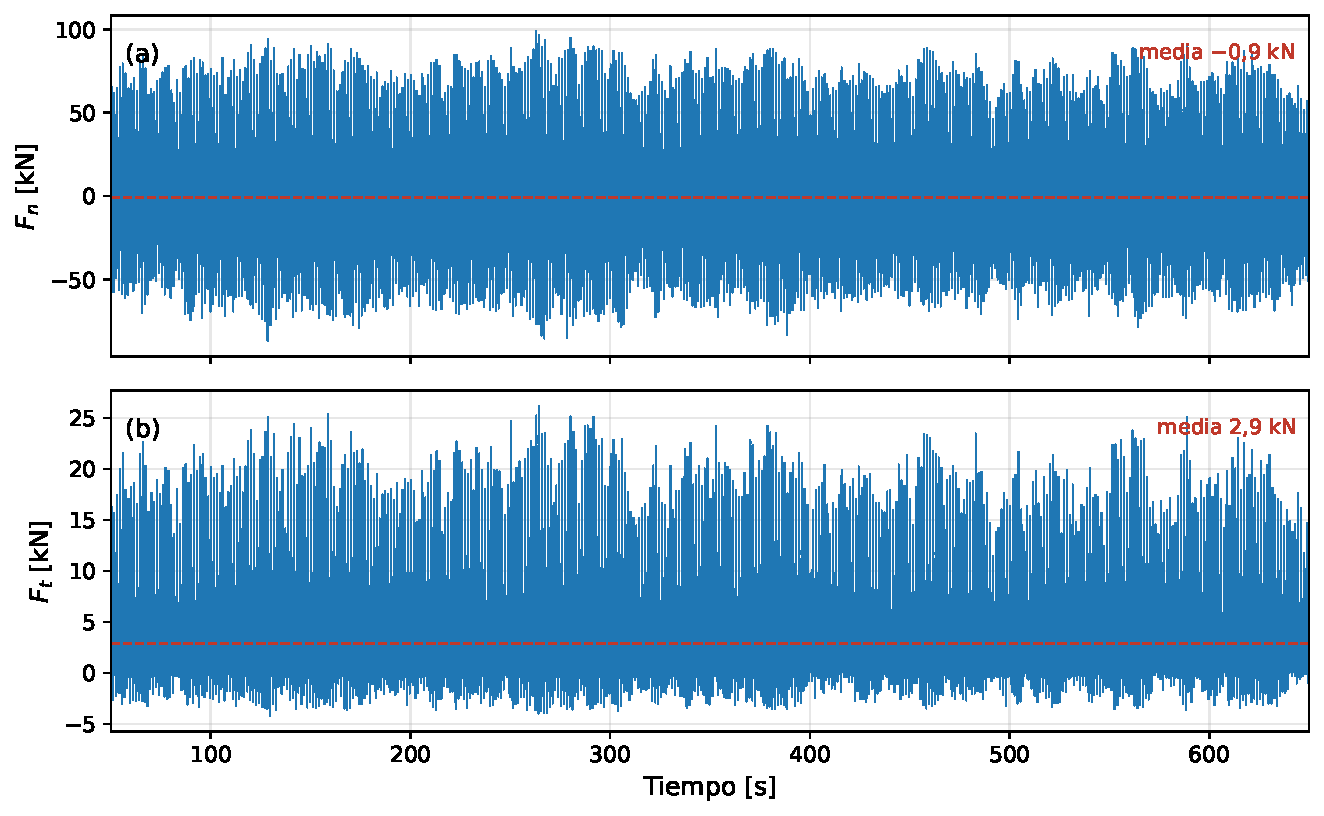
\includegraphics[width=0.85\textwidth]{Figuras/Figuras Anexo Fuerzas/fuerzas_xy_V22_S5.pdf}
    \caption{Fuerzas resultantes (a) $F_x$ y (b) $F_y$ en función del tiempo, $V = 22$~m/s, semilla $5$.}
    \label{fig:anexo_fuerzas_xy_V22_S5}
\end{figure}

\begin{figure}[H]
    \centering
    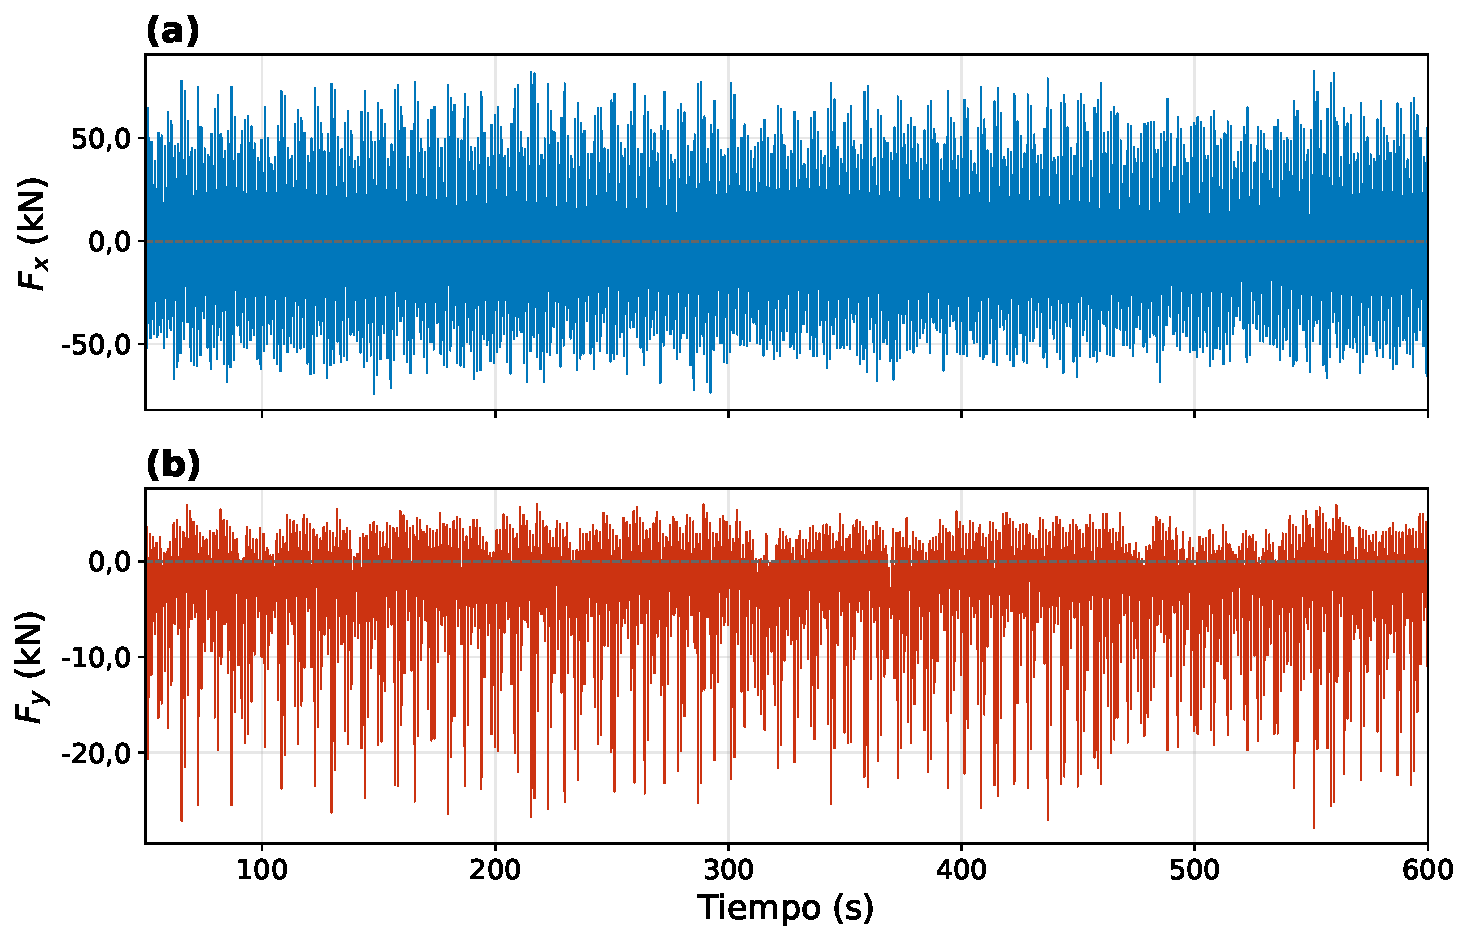
\includegraphics[width=0.85\textwidth]{Figuras/Figuras Anexo Fuerzas/fuerzas_xy_V22_S6.pdf}
    \caption{Fuerzas resultantes (a) $F_x$ y (b) $F_y$ en función del tiempo, $V = 22$~m/s, semilla $6$.}
    \label{fig:anexo_fuerzas_xy_V22_S6}
\end{figure}

\begin{figure}[H]
    \centering
    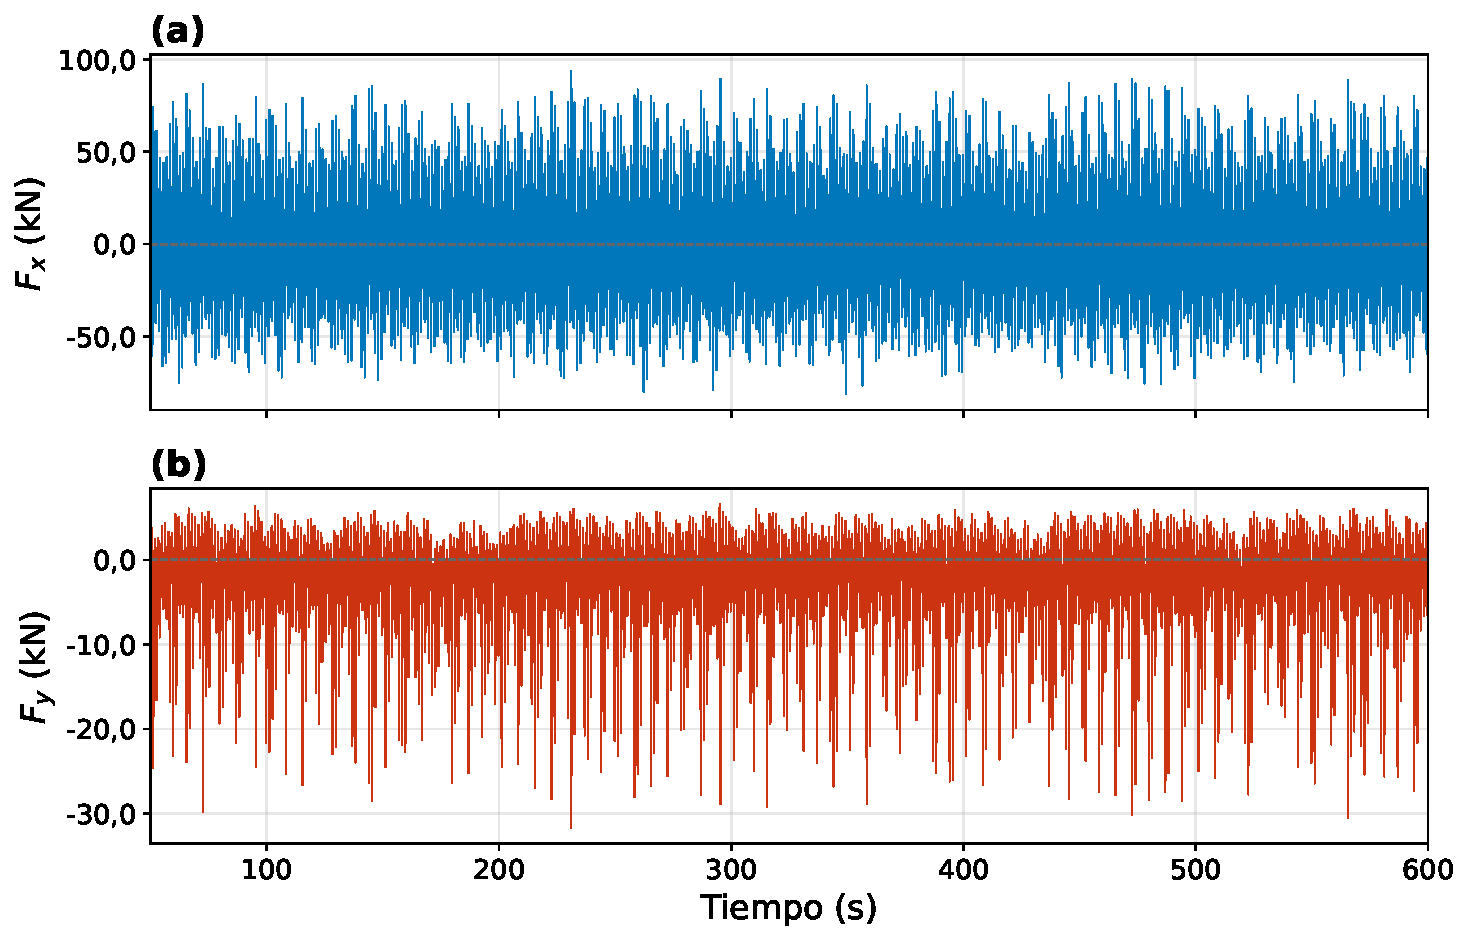
\includegraphics[width=0.85\textwidth]{Figuras/Figuras Anexo Fuerzas/fuerzas_xy_V24_S1.pdf}
    \caption{Fuerzas resultantes (a) $F_x$ y (b) $F_y$ en función del tiempo, $V = 24$~m/s, semilla $1$.}
    \label{fig:anexo_fuerzas_xy_V24_S1}
\end{figure}

\begin{figure}[H]
    \centering
    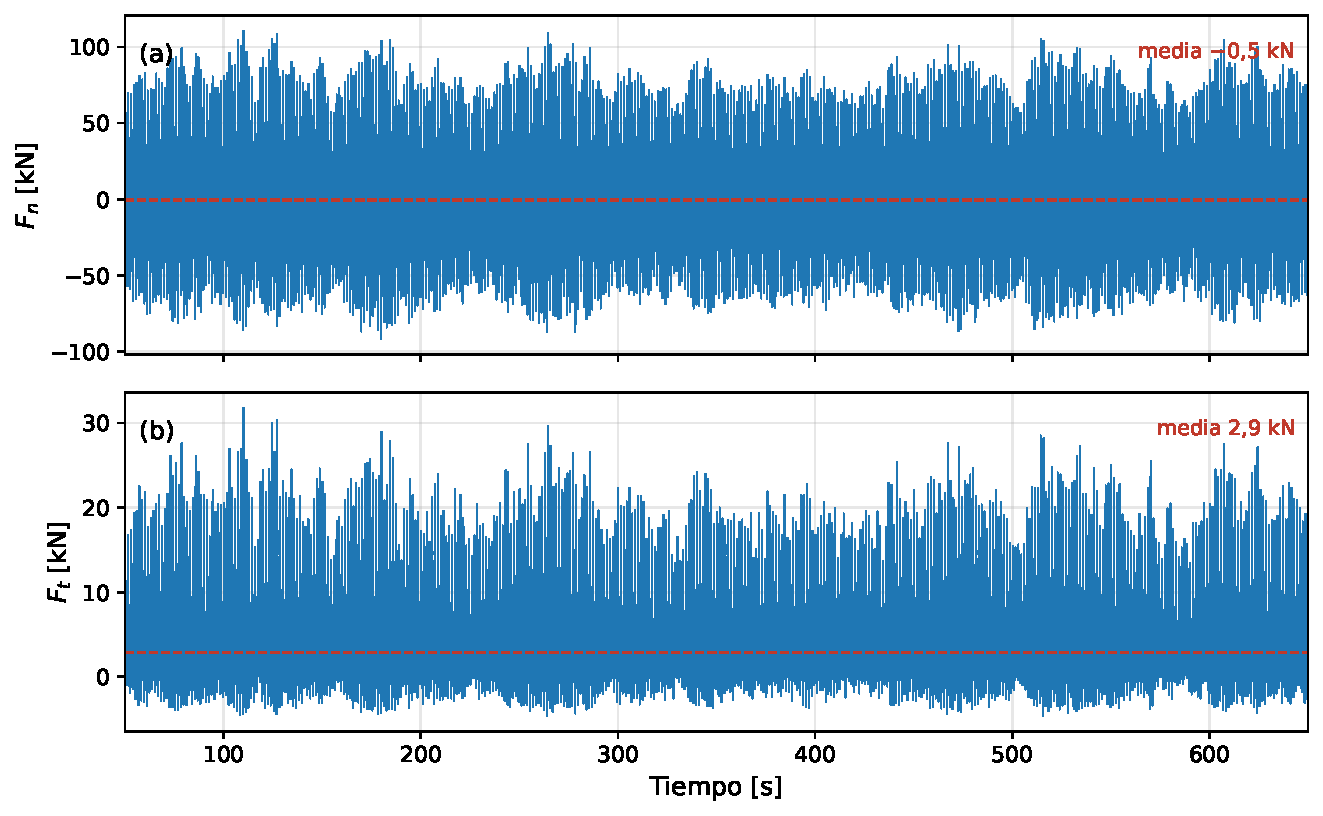
\includegraphics[width=0.85\textwidth]{Figuras/Figuras Anexo Fuerzas/fuerzas_xy_V24_S2.pdf}
    \caption{Fuerzas resultantes (a) $F_x$ y (b) $F_y$ en función del tiempo, $V = 24$~m/s, semilla $2$.}
    \label{fig:anexo_fuerzas_xy_V24_S2}
\end{figure}

\begin{figure}[H]
    \centering
    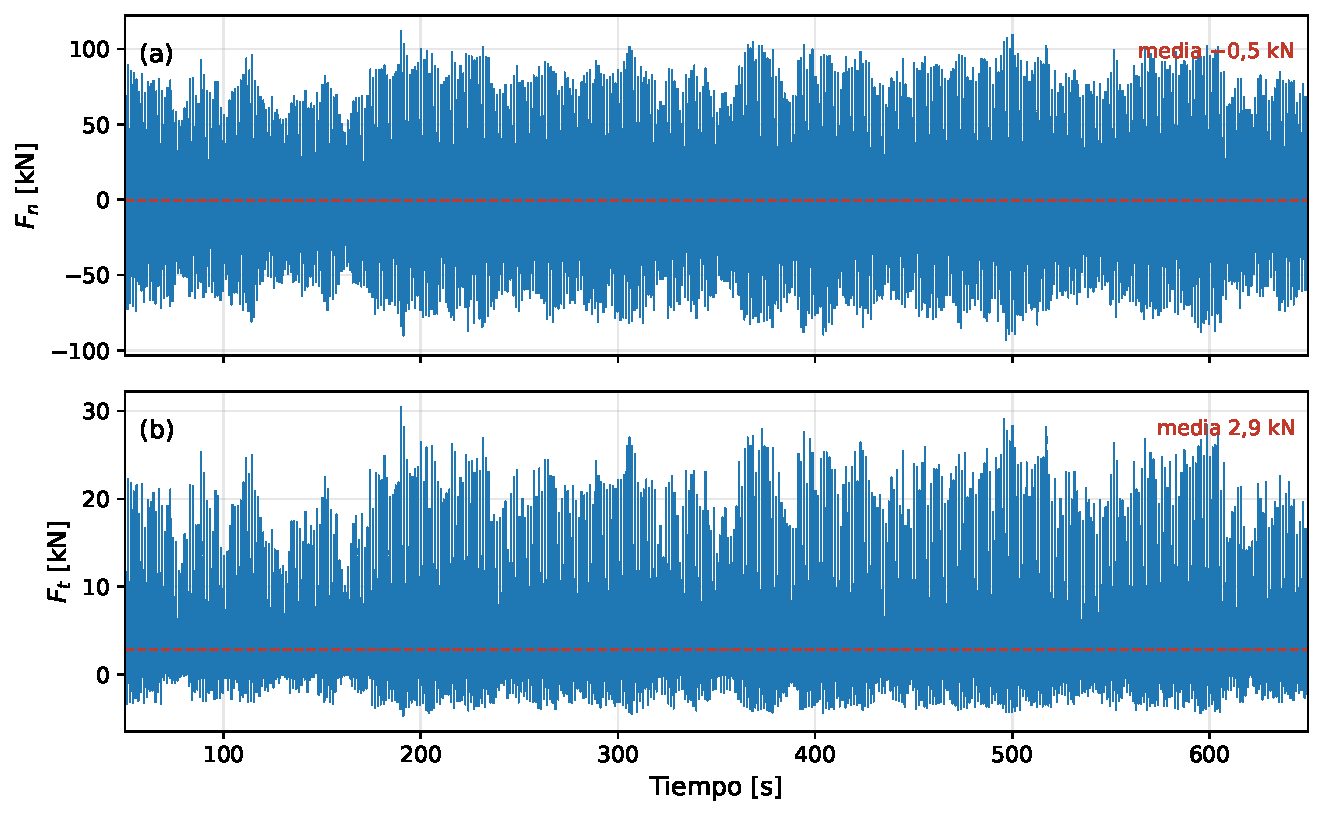
\includegraphics[width=0.85\textwidth]{Figuras/Figuras Anexo Fuerzas/fuerzas_xy_V24_S3.pdf}
    \caption{Fuerzas resultantes (a) $F_x$ y (b) $F_y$ en función del tiempo, $V = 24$~m/s, semilla $3$.}
    \label{fig:anexo_fuerzas_xy_V24_S3}
\end{figure}

\begin{figure}[H]
    \centering
    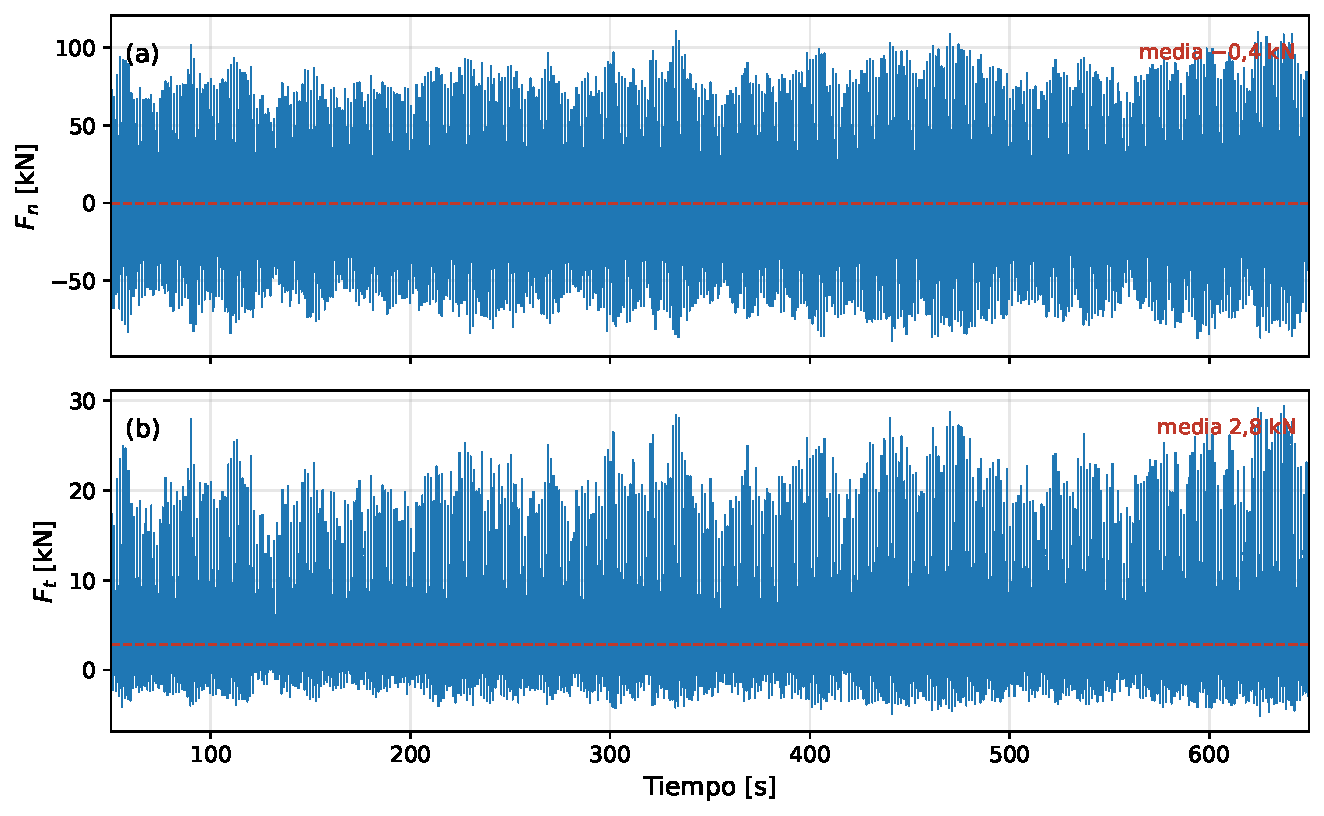
\includegraphics[width=0.85\textwidth]{Figuras/Figuras Anexo Fuerzas/fuerzas_xy_V24_S4.pdf}
    \caption{Fuerzas resultantes (a) $F_x$ y (b) $F_y$ en función del tiempo, $V = 24$~m/s, semilla $4$.}
    \label{fig:anexo_fuerzas_xy_V24_S4}
\end{figure}

\begin{figure}[H]
    \centering
    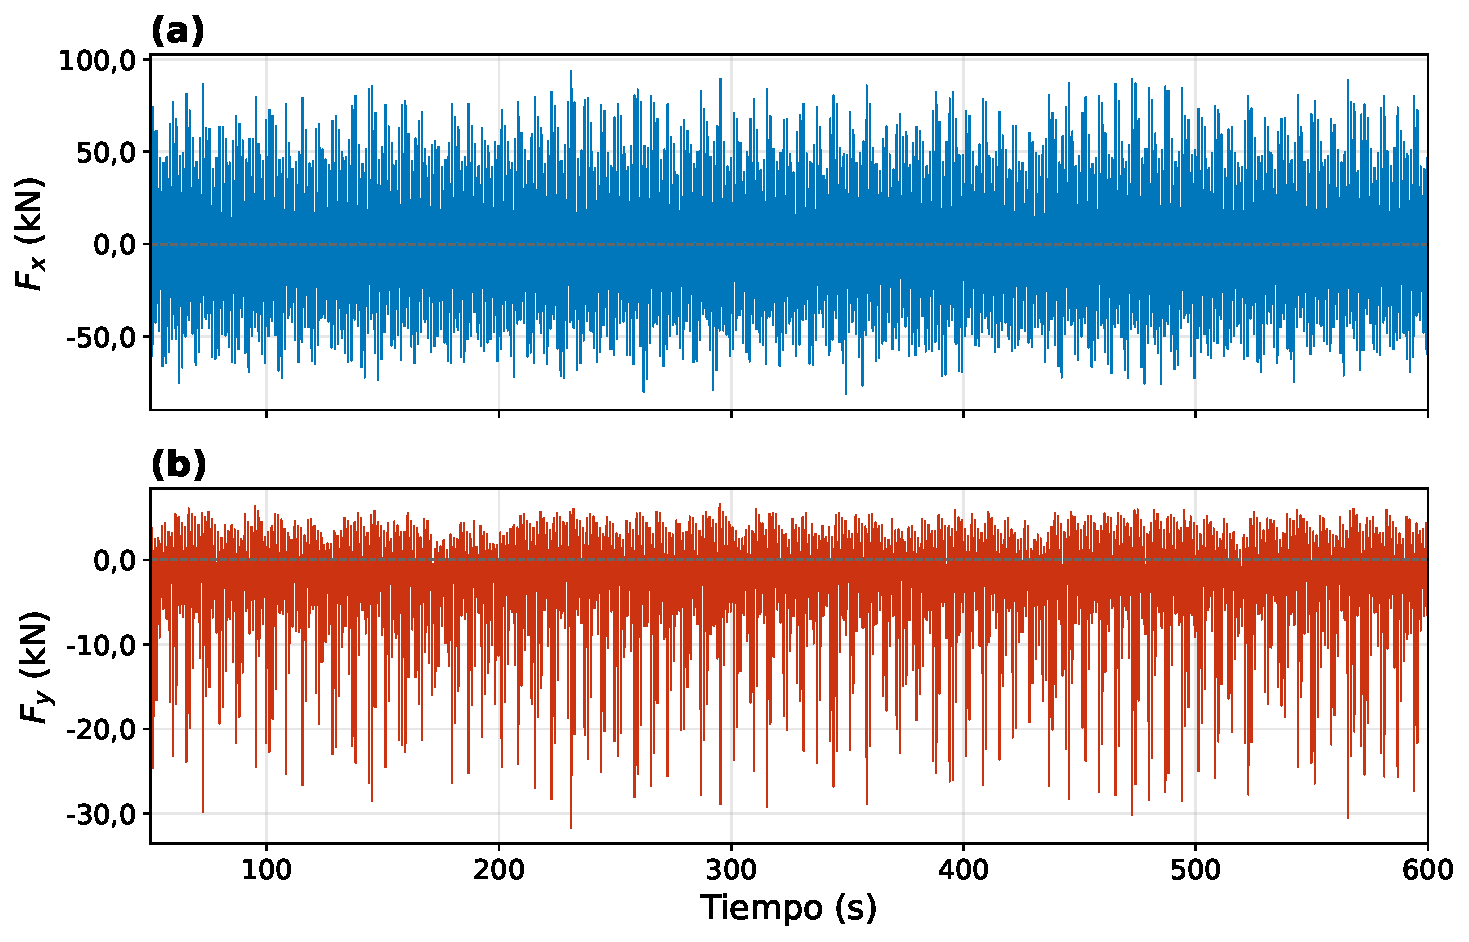
\includegraphics[width=0.85\textwidth]{Figuras/Figuras Anexo Fuerzas/fuerzas_xy_V24_S5.pdf}
    \caption{Fuerzas resultantes (a) $F_x$ y (b) $F_y$ en función del tiempo, $V = 24$~m/s, semilla $5$.}
    \label{fig:anexo_fuerzas_xy_V24_S5}
\end{figure}

\begin{figure}[H]
    \centering
    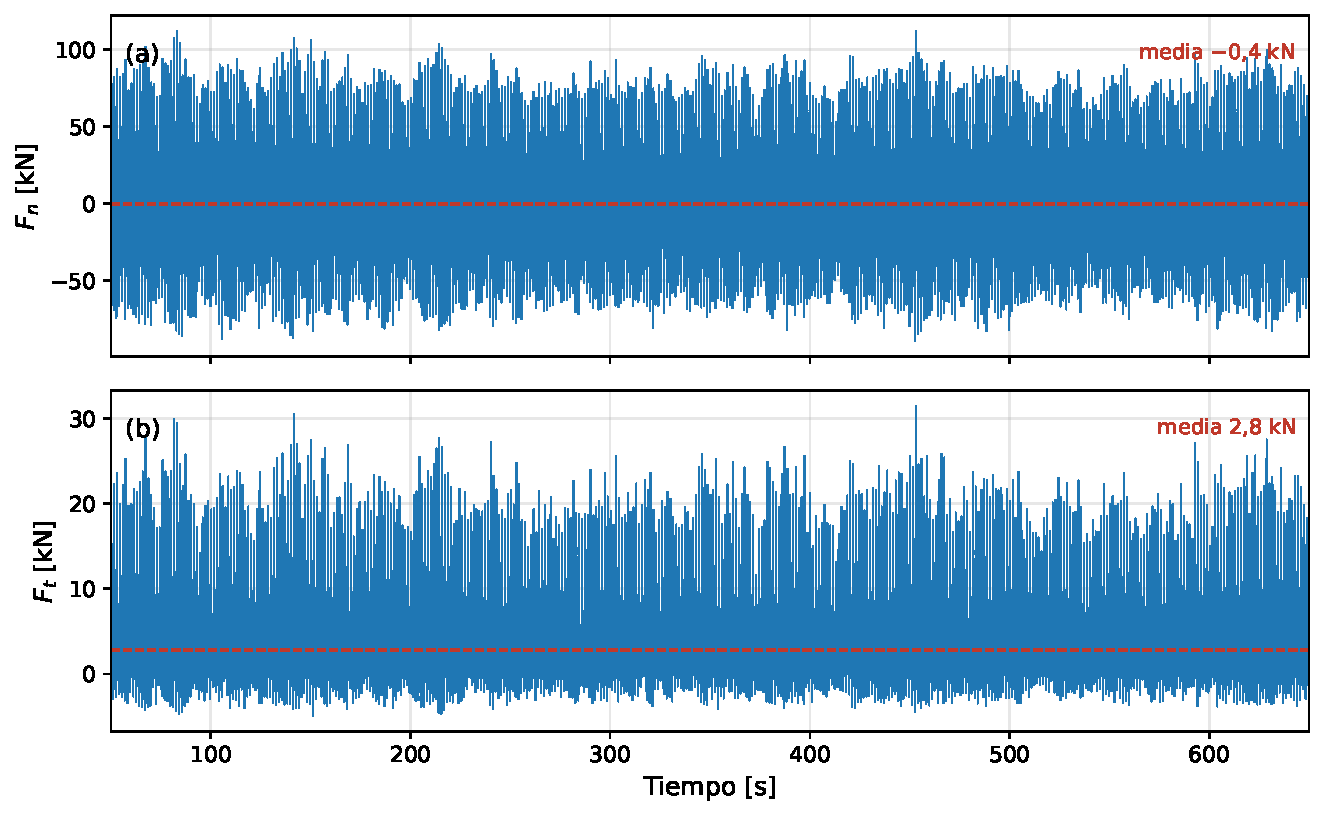
\includegraphics[width=0.85\textwidth]{Figuras/Figuras Anexo Fuerzas/fuerzas_xy_V24_S6.pdf}
    \caption{Fuerzas resultantes (a) $F_x$ y (b) $F_y$ en función del tiempo, $V = 24$~m/s, semilla $6$.}
    \label{fig:anexo_fuerzas_xy_V24_S6}
\end{figure}
